\section{Introduction}

La première release est dédiée aux fonctionnalités de la plateforme et à la mise en relation entre utilisateurs. Elle comprend un module d’authentification et d’administration, ainsi que les modules AniMatch, pour l’adoption et l’accouplement des animaux, et AniFound, pour la recherche des animaux perdus.

Cette release est réalisée à travers trois sprints :
\begin{itemize}
    \item \textbf{Sprint 1 : Authentification \& Administration}
    \item \textbf{Sprint 2 : Module AniMatch}
    \item \textbf{Sprint 3 : Module AniFound}
\end{itemize}


 
\section{Sprint 1 : Authentification et administration} Ce sprint, d’une durée de \textbf{deux semaines}, est consacré à la mise en place des fonctionnalités d’authentification et d’administration. Il permet d’assurer un accès sécurisé à la plateforme via la gestion des comptes utilisateurs (inscription, connexion et contrôle des rôles), ainsi que la mise en place d’un espace d’administration pour superviser le système et garantir la cohérence des opérations. 
\subsection{Sprint backlog} 
La table \ref{tab:sprint1-backlog} présente le Sprint Backlog du sprint 1 avec les user stories, les tâches associées et les efforts estimés :

\begin{longtable}{|p{1cm}|p{4.7cm}|p{7cm}|p{1.3cm}|}

\caption{Sprint Backlog du sprint 1}
\label{tab:sprint1-backlog} \\

\hline
\multicolumn{1}{|c|}{\cellcolor{coloranihub}\textbf{ID}} &
\multicolumn{1}{c|}{\cellcolor{coloranihub}\textbf{User Story}} &
\multicolumn{1}{c|}{\cellcolor{coloranihub}\textbf{Tâches}} &
\multicolumn{1}{c|}{\cellcolor{coloranihub}\textbf{Effort}} \\
\hline
\endfirsthead

\hline
\multicolumn{1}{|c|}{\cellcolor{coloranihub}\textbf{ID}} &
\multicolumn{1}{c|}{\cellcolor{coloranihub}\textbf{User Story}} &
\multicolumn{1}{c|}{\cellcolor{coloranihub}\textbf{Tâches}} &
\multicolumn{1}{c|}{\cellcolor{coloranihub}\textbf{Effort}} \\
\hline
\endhead

% ===================== US1 =====================
\multirow{5}{2cm}{US1}
& \multirow{5}{5cm}{En tant qu’utilisateur, je veux accéder à une interface moderne et intuitive, afin de naviguer facilement sur AniHub.}
& Conception du design sur Figma & 2 j \\
\cline{3-4}
& & Développement de l’interface d’accueil & 0.5 j \\
\cline{3-4}
& & Mise en place de la navigation et des pages principales & 0.5 j \\
\cline{3-4}
& & Harmonisation de l’interface utilisateur & 0.5 j \\
\cline{3-4}
& & Tests d’ergonomie et validation & 0.5 j \\
\hline

% ===================== US2 =====================
\multirow{5}{2cm}{US2}
& \multirow{5}{5cm}{En tant qu’utilisateur, je veux créer un compte afin d’accéder à la plateforme}
& Analyse des besoins & 0.5 j \\
\cline{3-4}
& & Conception de la maquette sur Figma& 0.5 j \\
\cline{3-4}
& & Développement de l’API d’inscription & 1 j \\
\cline{3-4}
& & Intégration frontend & 0.5 j \\
\cline{3-4}
& & Tests fonctionnels et validation & 0.5 j \\
\hline

% ===================== US3 =====================
\multirow{5}{2cm}{US3}
& \multirow{5}{5cm}{En tant qu’utilisateur, je veux me connecter afin d’utiliser l’application}
& Analyse des besoins & 0.5 j \\
\cline{3-4}
& & Conception de la maquette sur Figma & 0.5 j \\
\cline{3-4}
& & Développement de l’API d’authentification. & 0.5 j \\
\cline{3-4}
& & Gestion des sessions et des tokens & 0.5 j \\
\cline{3-4}
& & Tests de validation & 0.5 j \\
\hline

% ===================== US4 =====================
\multirow{4}{2cm}{US4}
& \multirow{4}{5cm}{En tant qu’utilisateur, je veux gérer mon profil afin de personnaliser mes informations}
& Conception des interfaces de gestion du profil sur Figma & 0.5 j \\
\cline{3-4}
& & API de mise à jour du profil.& 1 j \\
\cline{3-4}
& & Intégration frontend & 0.5 j \\
\cline{3-4}
& & Tests et validation & 0.5 j \\
\hline

% ===================== US5 =====================
\multirow{5}{2cm}{US5}
& \multirow{5}{5cm}{En tant qu’administrateur, je veux gérer tous les utilisateurs afin de superviser la plateforme}
& Analyse des besoins & 0.5 j \\
\cline{3-4}
& & Maquette du tableau de bord sur Figma. & 1 j \\
\cline{3-4}
& & API de gestion des utilisateurs (CRUD) & 1 j \\
\cline{3-4}
& & Implémentation du dashboard administrateur & 0.5 j \\
\cline{3-4}
& & Tests fonctionnels & 0.5 j \\
\hline

% ===================== US6 =====================
\multirow{5}{2cm}{US6}
& \multirow{5}{5cm}{En tant qu’administrateur, je veux gérer toutes les annonces afin de superviser et contrôler le contenu}
& Analyse des besoins & 0.5 j \\
\cline{3-4}
& & Maquettes des interfaces de gestion des annonces sur Figma. & 0.5 j \\
\cline{3-4}
& &API de gestion des annonces (CRUD) & 1 j \\
\cline{3-4}
& & Intégration frontend & 0.5 j \\
\cline{3-4}
& & Tests et validation& 0.5 j \\
\hline

\end{longtable}

\newpage
\subsection{Diagramme des cas d’utilisation du sprint 1}
Dans cette section, nous présentons le diagramme des cas d’utilisation du premier sprint, dédié au module \textbf{Authentification et administration}. 

La figure \ref{fig:usecase-sprint1} illustre les différentes fonctionnalités liées à l’authentification et à l’administration :  

\begin{figure}[H]
    \centering
    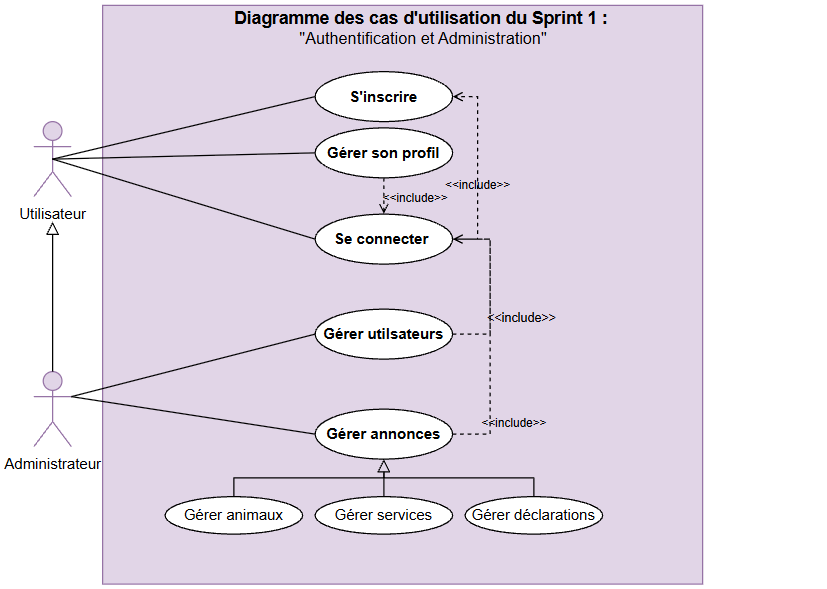
\includegraphics[width=9\linewidth, height=15.5cm, keepaspectratio]{images/use case sprint 1.png}
    \caption{Diagramme des cas d’utilisation du sprint 1}
    \label{fig:usecase-sprint1}
\end{figure}



\subsection{Descriptions textuelles des cas d’utilisation du sprint 1}


\subsubsection{Description textuelle du cas d’utilisation « S’inscrire »} 
La table \ref{tab:DTinscription} présente la description textuelle du cas d’utilisation "S’inscrire" : 
\newpage  
\begin{longtable}{|c|p{11cm}|}
\caption{Description textuelle du cas d’utilisation "S’inscrire"}
\label{tab:DTinscription} \\
\hline
\cellcolor{coloranihub} \textbf{Nom du cas d'utilisation } & S’inscrire \\
\hline
\cellcolor{coloranihub} \textbf{Acteurs} & Utilisateur \\
\hline
\cellcolor{coloranihub} \textbf{Description } & Il  s’inscrit sur AniHub afin d’accéder aux fonctionnalités. \\
\hline
\cellcolor{coloranihub} \textbf{Pré-condition } & L’utilisateur doit accéder à la page d’inscription. \\
\hline
\cellcolor{coloranihub} \textbf{Post-condition } & Un compte utilisateur est créé avec succès . \\
\hline
\cellcolor{coloranihub} \textbf{Scénario nominal } & 
\begin{enumerate}
\item L’utilisateur accède à la page d’inscription.
\item L’utilisateur saisit ses informations personnelles (nom, email, mot de passe, etc.) et valide .
\item Le système vérifie la validité des données saisies.
\item Le système crée un nouveau compte utilisateur.
\item Le système confirme la création du compte.
\item L’utilisateur est redirigé vers la page de connexion
\end{enumerate} \\
\hline
\end{longtable}


\subsubsection{Description textuelle du cas d’utilisation « Se connecter »} 
La table \ref{tab:connexion} présente la description textuelle du cas d’utilisation "Se connecter" :
\begin{longtable}{|c|p{11cm}|}
\caption{Description textuelle du cas d’utilisation "Se connecter"}
\label{tab:connexion} \\
\hline
\cellcolor{coloranihub} \textbf{Nom du cas d'utilisation } & Se connecter \\
\hline
\cellcolor{coloranihub} \textbf{Acteurs} & Utilisateur \\
\hline
\cellcolor{coloranihub} \textbf{Description } & Tout utilisateur disposant d’un compte peut s’authentifier . \\
\hline
\cellcolor{coloranihub} \textbf{Pré-condition } & L’utilisateur doit posséder un compte . \\
\hline
\cellcolor{coloranihub} \textbf{Post-condition } & il est authentifié et redirigé vers l’interface principale. \\
\hline
\cellcolor{coloranihub} \textbf{Scénario nominal } & 
\begin{enumerate}
\item L’utilisateur accède à la page de connexion.
\item Le système affiche le formulaire d’authentification.
\item L’utilisateur saisit son email et son mot de passe.
\item L’utilisateur valide le formulaire de connexion.
\item Le système vérifie les informations d’identification.
\item Le système authentifie l’utilisateur.
\item Le système redirige l’utilisateur vers la page d’accueil.
\end{enumerate} \\
\hline
\end{longtable}



\newpage


\newpage 

\subsubsection{Description textuelle du cas d’utilisation « Gérer son profil »}
La table \ref{tab:gerer_profil} présente la description textuelle du cas d’utilisation "Gérer son profil" :
\begin{longtable}{|c|p{11cm}|}
\caption{Description textuelle du cas d'utilisation "Gérer son profil"}
\label{tab:gerer_profil} \\
\hline
\cellcolor{coloranihub}\textbf{Nom du cas d'utilisation } & Gérer son profil (modifier / supprimer) \\
\hline
\cellcolor{coloranihub}\textbf{Acteurs} & Utilisateur \\
\hline
\cellcolor{coloranihub}\textbf{Description } & L’utilisateur peut consulter, modifier ou supprimer son profil. \\
\hline
\cellcolor{coloranihub}\textbf{Pré-condition } & L’utilisateur doit être authentifié. \\
\hline
\cellcolor{coloranihub}\textbf{Post-condition } & Les informations du profil sont mises à jour ou le compte est supprimé avec succès. \\
\hline

\cellcolor{coloranihub}\textbf{Scénario nominal } &
\begin{enumerate}
\item L’utilisateur accède à la page d’accueil d’AniHub.
\item L’utilisateur sélectionne « Mon espace » dans la barre de navigation.
\item Le système redirige l’utilisateur vers son profil.
\item Le système affiche les informations personnelles de l’utilisateur.
\item L’utilisateur choisit une action.
\item Cas modification :
\begin{itemize}
\item L’utilisateur clique sur « Modifier profil ».
\item Le système affiche le formulaire pré-rempli.
\item L’utilisateur modifie ses informations.
\item L’utilisateur valide les modifications.
\item Le système vérifie et enregistre les nouvelles données. 
\item le système affiche un message confirmant la mise à jour des informations avec succès . 
\end{itemize}
\item Cas suppression :
\begin{itemize}
\item L’utilisateur clique sur « Supprimer mon compte ».
\item Le système demande une confirmation.
\item L’utilisateur confirme la suppression.
\item Le système supprime définitivement le compte et le redirige vers la page d’inscription..
\end{itemize}
\end{enumerate} \\
\hline

\cellcolor{coloranihub}\textbf{Scénario alternatif :} &
\begin{itemize}
\item Erreur lors de la modification : le système affiche un message d’erreur.
\item Annulation de la suppression : e compte de l’utilisateur est conservé.
\end{itemize} \\
\hline

\end{longtable}






\newpage 

\subsubsection{Description textuelle du cas d’utilisation « Gérer les utilisateurs »}
La table \ref{tab:gerer_utilisateurs} présente la description textuelle du cas d’utilisation "Gérer les utilisateurs" :
\begin{longtable}{|c|p{11cm}|}
\caption{Description textuelle du cas d'utilisation "Gérer les utilisateurs"}
\label{tab:gerer_utilisateurs} \\
\hline
\cellcolor{coloranihub}\textbf{Nom du cas d'utilisation } & Gérer les utilisateurs \\
\hline
\cellcolor{coloranihub}\textbf{Acteurs} & Administrateur \\
\hline
\cellcolor{coloranihub}\textbf{Description } & L’administrateur peut gérer les comptes utilisateurs (consultation, modification, suppression). \\
\hline
\cellcolor{coloranihub}\textbf{Pré-condition } & L’administrateur doit être authentifié. \\
\hline
\cellcolor{coloranihub}\textbf{Post-condition } & Les données de l’utilisateur sont mises à jour ou supprimées avec succès. \\
\hline

\cellcolor{coloranihub}\textbf{Scénario nominal } &
\begin{enumerate}
\item L’administrateur accède à la page d’accueil d’AniHub.
\item L’administrateur accède à son espace administrateur.
\item Le système affiche le tableau de bord administrateur.
\item L’administrateur consulte le tableau de bord pour voir les statistiques des utilisateurs.
\item L’administrateur accède ensuite à la section « Gestion des utilisateurs ».
\item Le système affiche la liste des utilisateurs.
\item L’administrateur sélectionne un utilisateur.

\item Cas modification :
\begin{itemize}
\item L’administrateur clique sur « Modifier ».
\item Le système affiche le formulaire de modification.
\item L’administrateur met à jour ses informations.
\item Le système enregistre les modifications.
\end{itemize}

\item Cas suppression :
\begin{itemize}
\item L’administrateur clique sur « Supprimer ».
\item Le système demande une confirmation.
\item L’administrateur confirme la suppression.
\item Le système supprime définitivement le compte utilisateur.
\end{itemize}

\item Le système affiche un message de confirmation .
\end{enumerate} \\
\hline

\cellcolor{coloranihub}\textbf{Scénario alternatif :} &
\begin{itemize}
\item Annulation de la suppression : aucune action n’est effectuée et le compte est conservé.
\item Erreur lors de la modification : le système affiche un message d’erreur.
\end{itemize} \\
\hline
\end{longtable} 
\newpage 



\subsubsection{Description textuelle du cas d’utilisation « Gérer les annonces »}
La table \ref{tab:gerer_annonces_admin} présente la description textuelle du cas d’utilisation "Gérer les annonces" :

\begin{longtable}{|c|p{11cm}|}
\caption{Description textuelle du cas d'utilisation "Gérer les annonces"}
\label{tab:gerer_annonces_admin} \\
\hline
\cellcolor{coloranihub}\textbf{Nom du cas d'utilisation } & Gérer les annonces \\
\hline
\cellcolor{coloranihub}\textbf{Acteurs} & Administrateur \\
\hline
\cellcolor{coloranihub}\textbf{Description } & L’administrateur peut consulter et gérer les différentes annonces de la plateforme .\\
\hline
\cellcolor{coloranihub}\textbf{Pré-condition } & L’administrateur doit être authentifié. \\
\hline
\cellcolor{coloranihub}\textbf{Post-condition } & Les annonces supprimées ne sont plus visibles sur la plateforme. \\
\hline

\cellcolor{coloranihub}\textbf{Scénario nominal } &
\begin{enumerate}
\item L’administrateur accède à la page d’accueil d’AniHub.
\item L’administrateur se connecte à son espace administrateur.
\item Le système affiche le tableau de bord administrateur avec des statistiques générales.
\item L’administrateur accède à la section « Gestion des annonces ».
\item Le système affiche les différents types d’annonces disponibles.
\item L’administrateur choisit un type d’annonce (adoption, accouplement, vente, déclaration ou service).
\item Le système affiche la liste des annonces correspondant au type sélectionné.

\item Cas suppression :
\begin{itemize}
\item L’administrateur sélectionne une annonce.
\item L’administrateur clique sur « Supprimer ».
\item Le système demande une confirmation.
\item L’administrateur confirme la suppression.
\item Le système supprime définitivement l’annonce.
\end{itemize}

\item Le système affiche un message de confirmation de l’opération.
\end{enumerate} \\
\hline

\cellcolor{coloranihub}\textbf{Scénario alternatif :} &
\begin{itemize}
\item Annulation de la suppression : aucune action n’est effectuée et l’annonce est conservée.
\item Erreur lors de la suppression : le système affiche un message d’erreur.
\end{itemize} \\
\hline

\end{longtable}
\newpage 
 
\subsection{Diagrammes des classes du sprint 1}  
Dans cette section, nous présentons le diagramme de classes du Sprint 1, qui regroupe l’ensemble des classes liées à l’authentification et à l’administration.

La figure \ref{fig:class_diagram_sprint1} illustre le diagramme de classes correspondant : 
\begin{figure}[H]
    \centering
    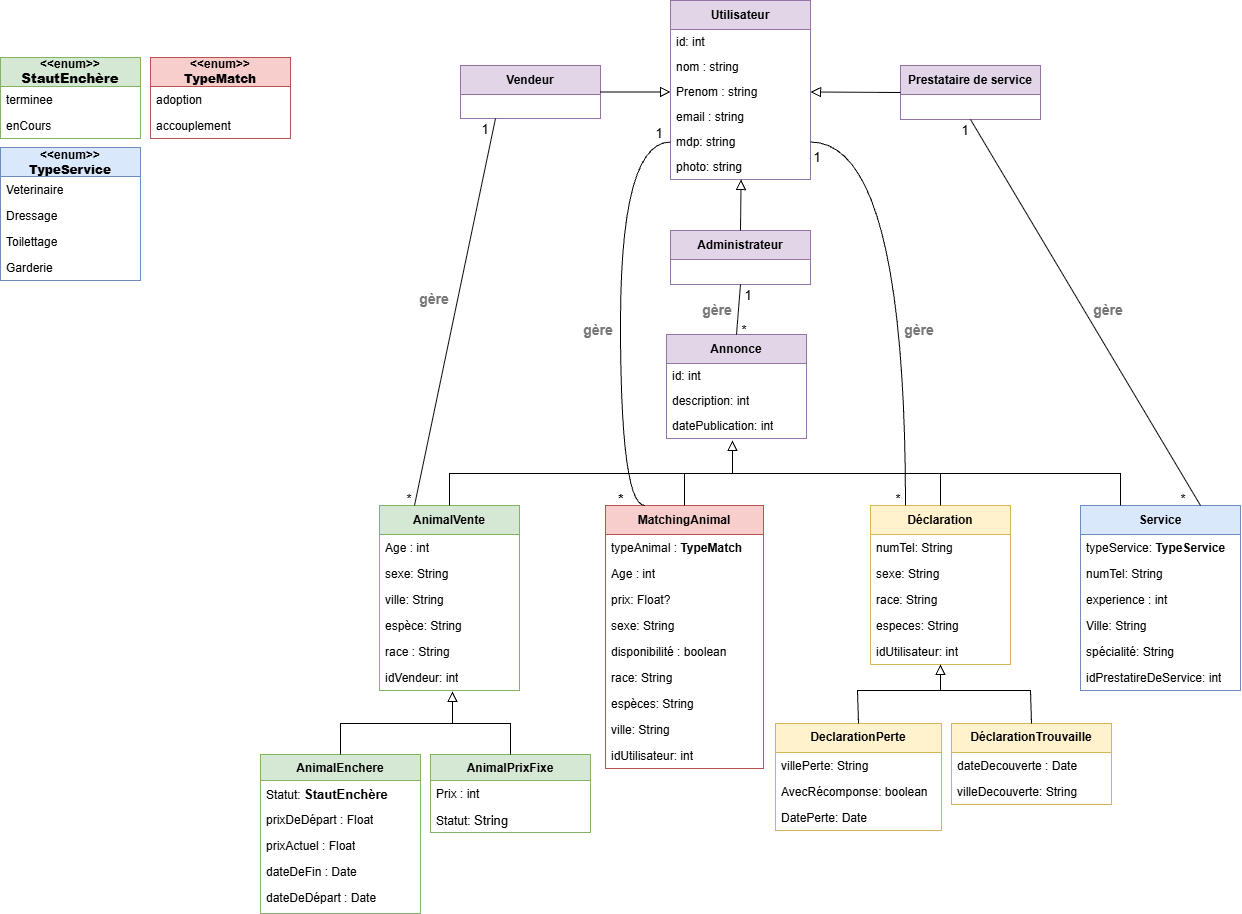
\includegraphics[width=1\textwidth, height=20cm, keepaspectratio]{images/class diagram sprint 1.png}
    \caption{Diagramme de classes du sprint 1}
    \label{fig:class_diagram_sprint1}
\end{figure} 

\subsection{Diagrammes de séquences du sprint 1}

Cette section présente les diagrammes de séquences du premier sprint, illustrant les interactions entre les différents composants du système.

\subsubsection{Diagramme de séquence : inscription}
La figure \ref{fig:sequence-inscription} illustre les interactions entre l’utilisateur et le système lors du processus d’inscription :  
\newpage
\begin{figure}[H]
\centering
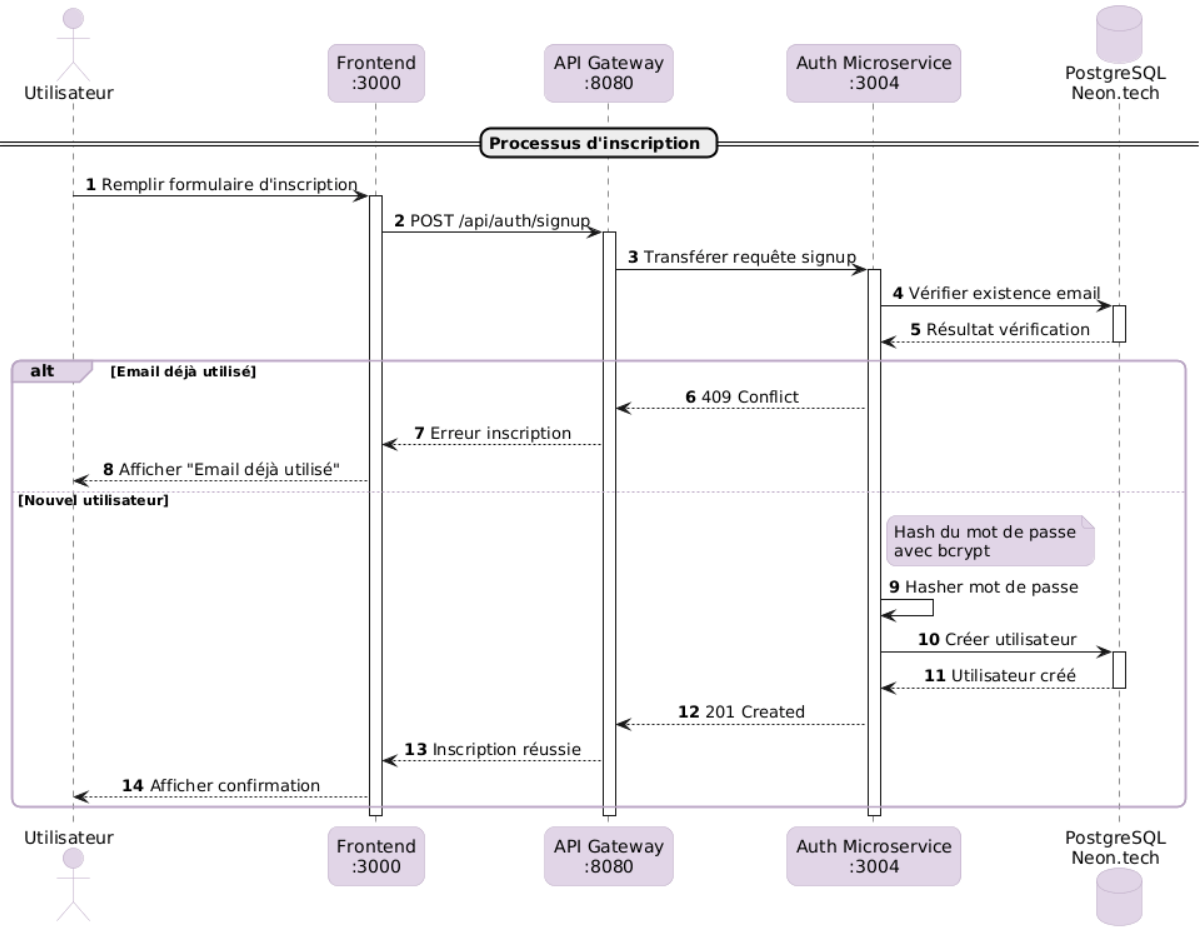
\includegraphics[width=0.6\textwidth]{images/sinscrire.png}
\caption{Diagramme de séquence de l’inscription}
\label{fig:sequence-inscription}
\end{figure}

\vspace{-0.5cm}

\subsubsection{Diagramme de séquence : connexion}
La figure \ref{fig:sequence-connexion} illustre les interactions entre l’utilisateur et le système lors du processus de connexion : 
\begin{figure}[H]
\centering
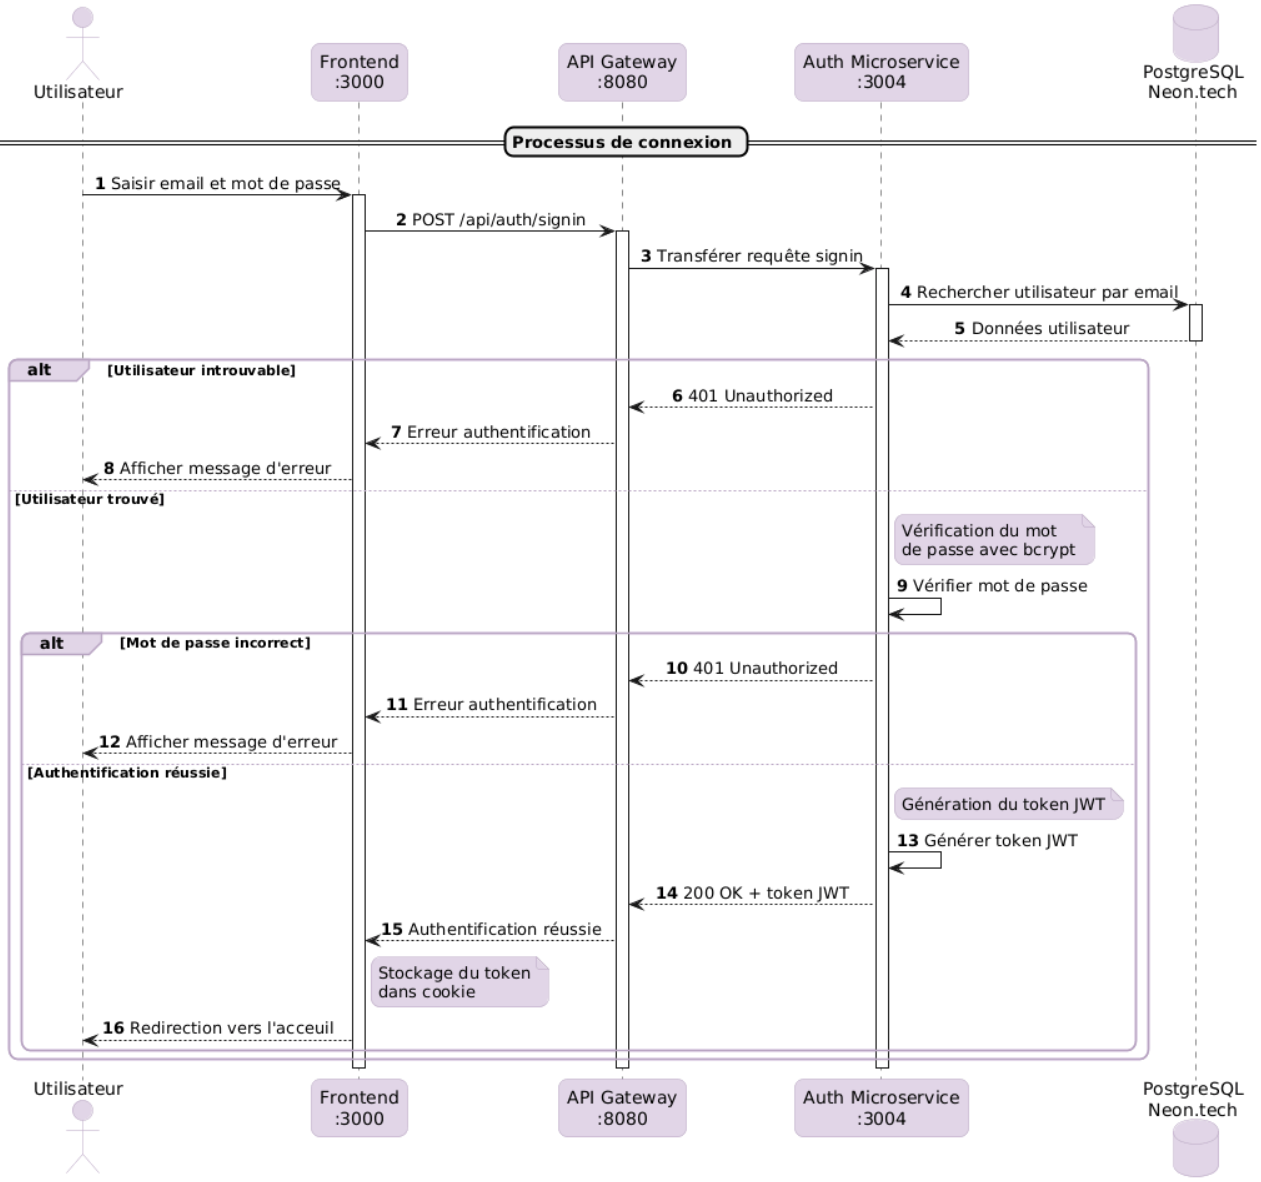
\includegraphics[width=0.6\textwidth]{images/connexion.png}
\caption{Diagramme de séquence de la connexion}
\label{fig:sequence-connexion}
\end{figure}
\newpage  
\subsubsection{Diagramme de séquence : gestion des utilisateurs}

La figure \ref{fig:sequence-gerer-users} illustre le processus de gestion des utilisateurs par l’administrateur. Elle décrit les différentes interactions entre le frontend, l’API Gateway et le microservice d’authentification, notamment lors des opérations de modification et de suppression d’un utilisateur. Le diagramme met en évidence la vérification des droits d’accès de l’administrateur ainsi que le traitement des actions autorisées ou refusées : 
\begin{figure}[H]
\centering
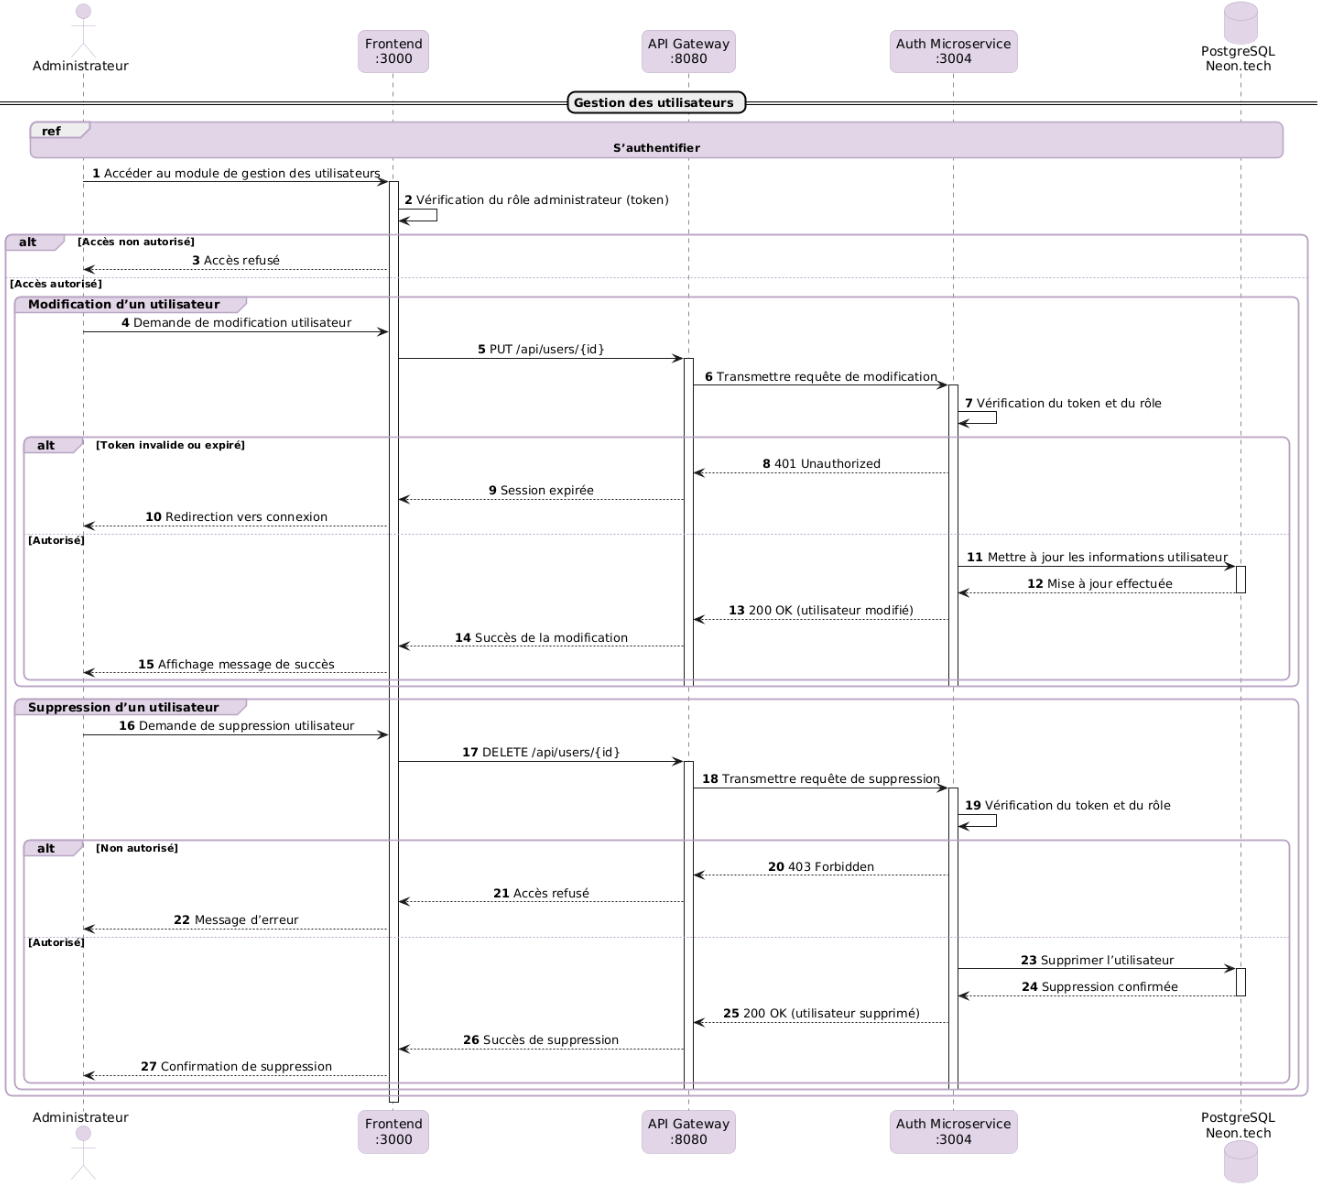
\includegraphics[width=\textwidth]{images/gererutilsateurs.png}
\caption{Diagramme de séquence de la gestion des utilisateurs}
\label{fig:sequence-gerer-users}
\end{figure} 
\newpage
\subsubsection{Diagramme de séquence : gestion des annonces} 

La figure \ref{fig:sequence-gerer-annonces} illustre le processus de gestion des annonces des modules AniMatch, AniFound, AniMarket et AniCare, incluant les opérations d’activation, de désactivation et de suppression. Elle met en évidence les interactions entre le frontend, l’API Gateway et les microservices concernés, ainsi que la publication des notifications aux utilisateurs via le service de notification : 
\begin{figure}[H]
\centering
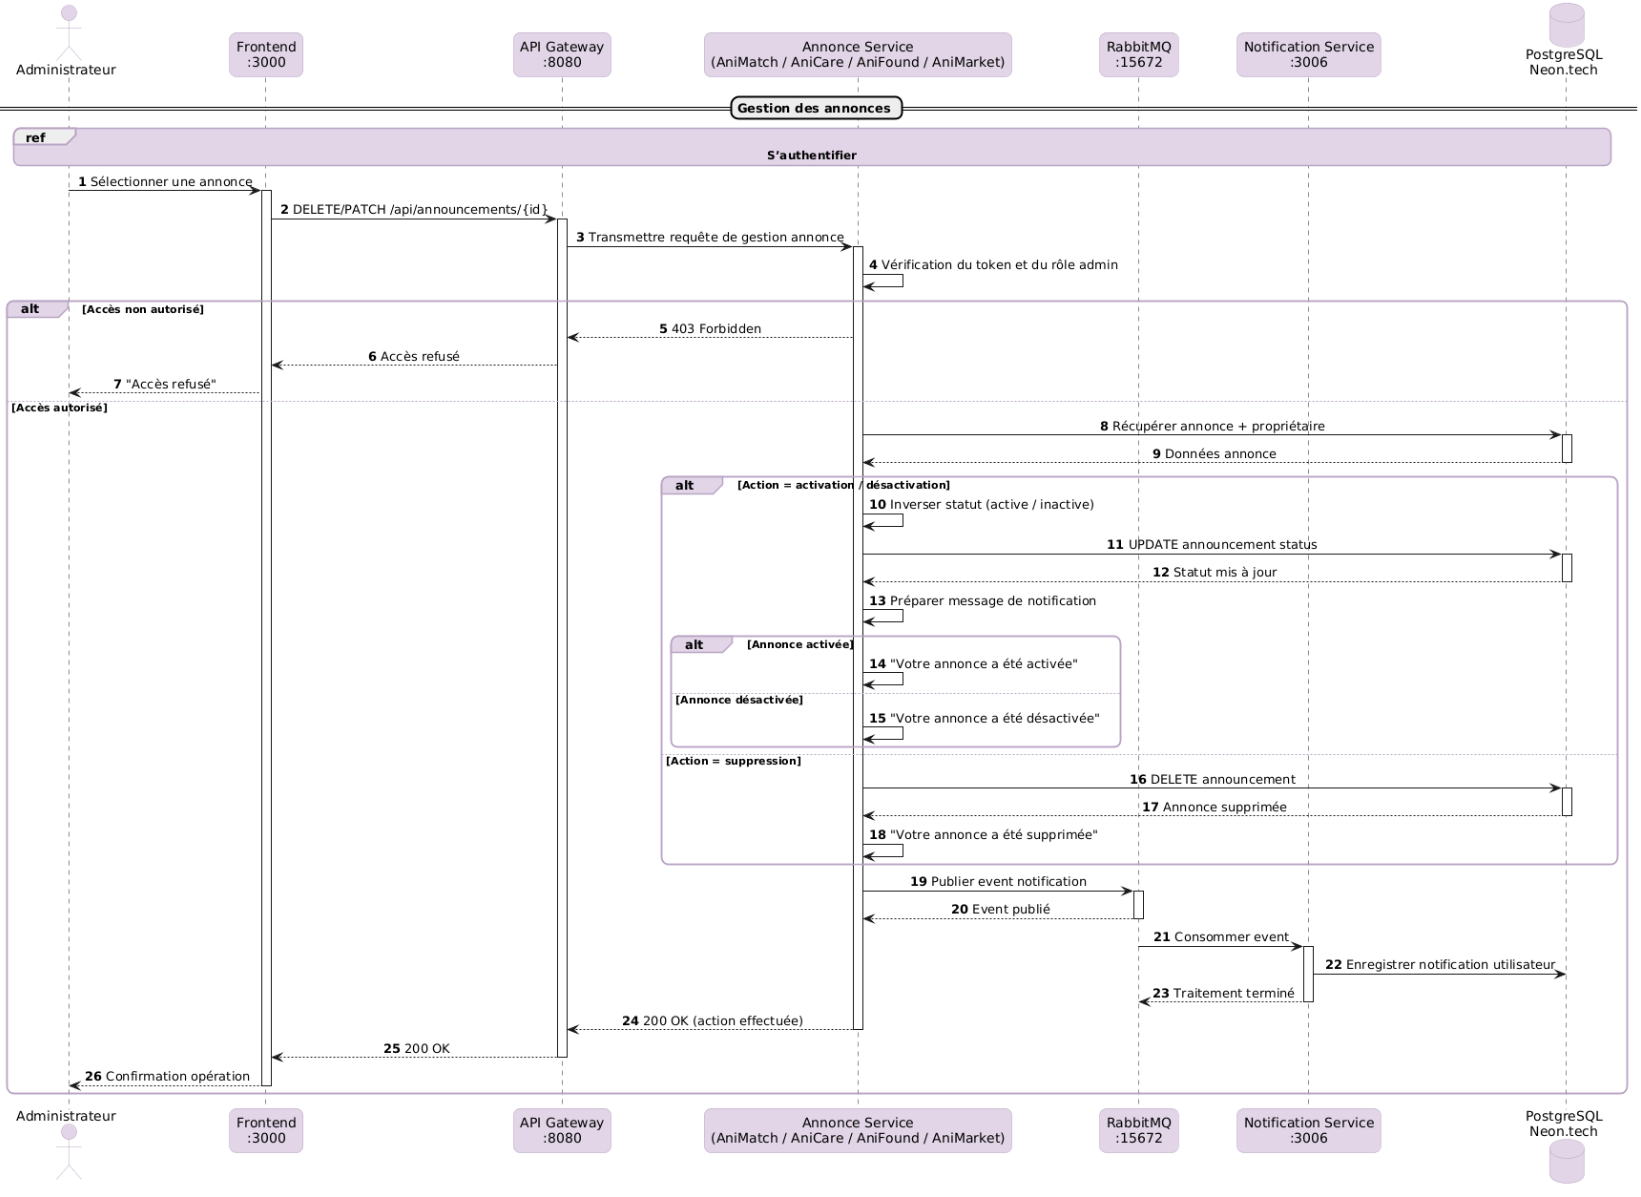
\includegraphics[width=\textwidth,height=0.99\textheight,keepaspectratio]{images/gererannonces.png}
\caption{Diagramme de séquence de la gestion des annonces}
\label{fig:sequence-gerer-annonces}
\end{figure} 
\newpage
\subsection{Réalisation su sprint 1 }  
\subsubsection{Réalisation des maquettes Figma pour les interfaces de la plateforme AniHub}

La figure \ref{fig:figma_maquettes} présente les maquettes réalisées avec Figma pour toutes les interfaces de la plateforme AniHub.

\begin{figure}[H]
    \centering
    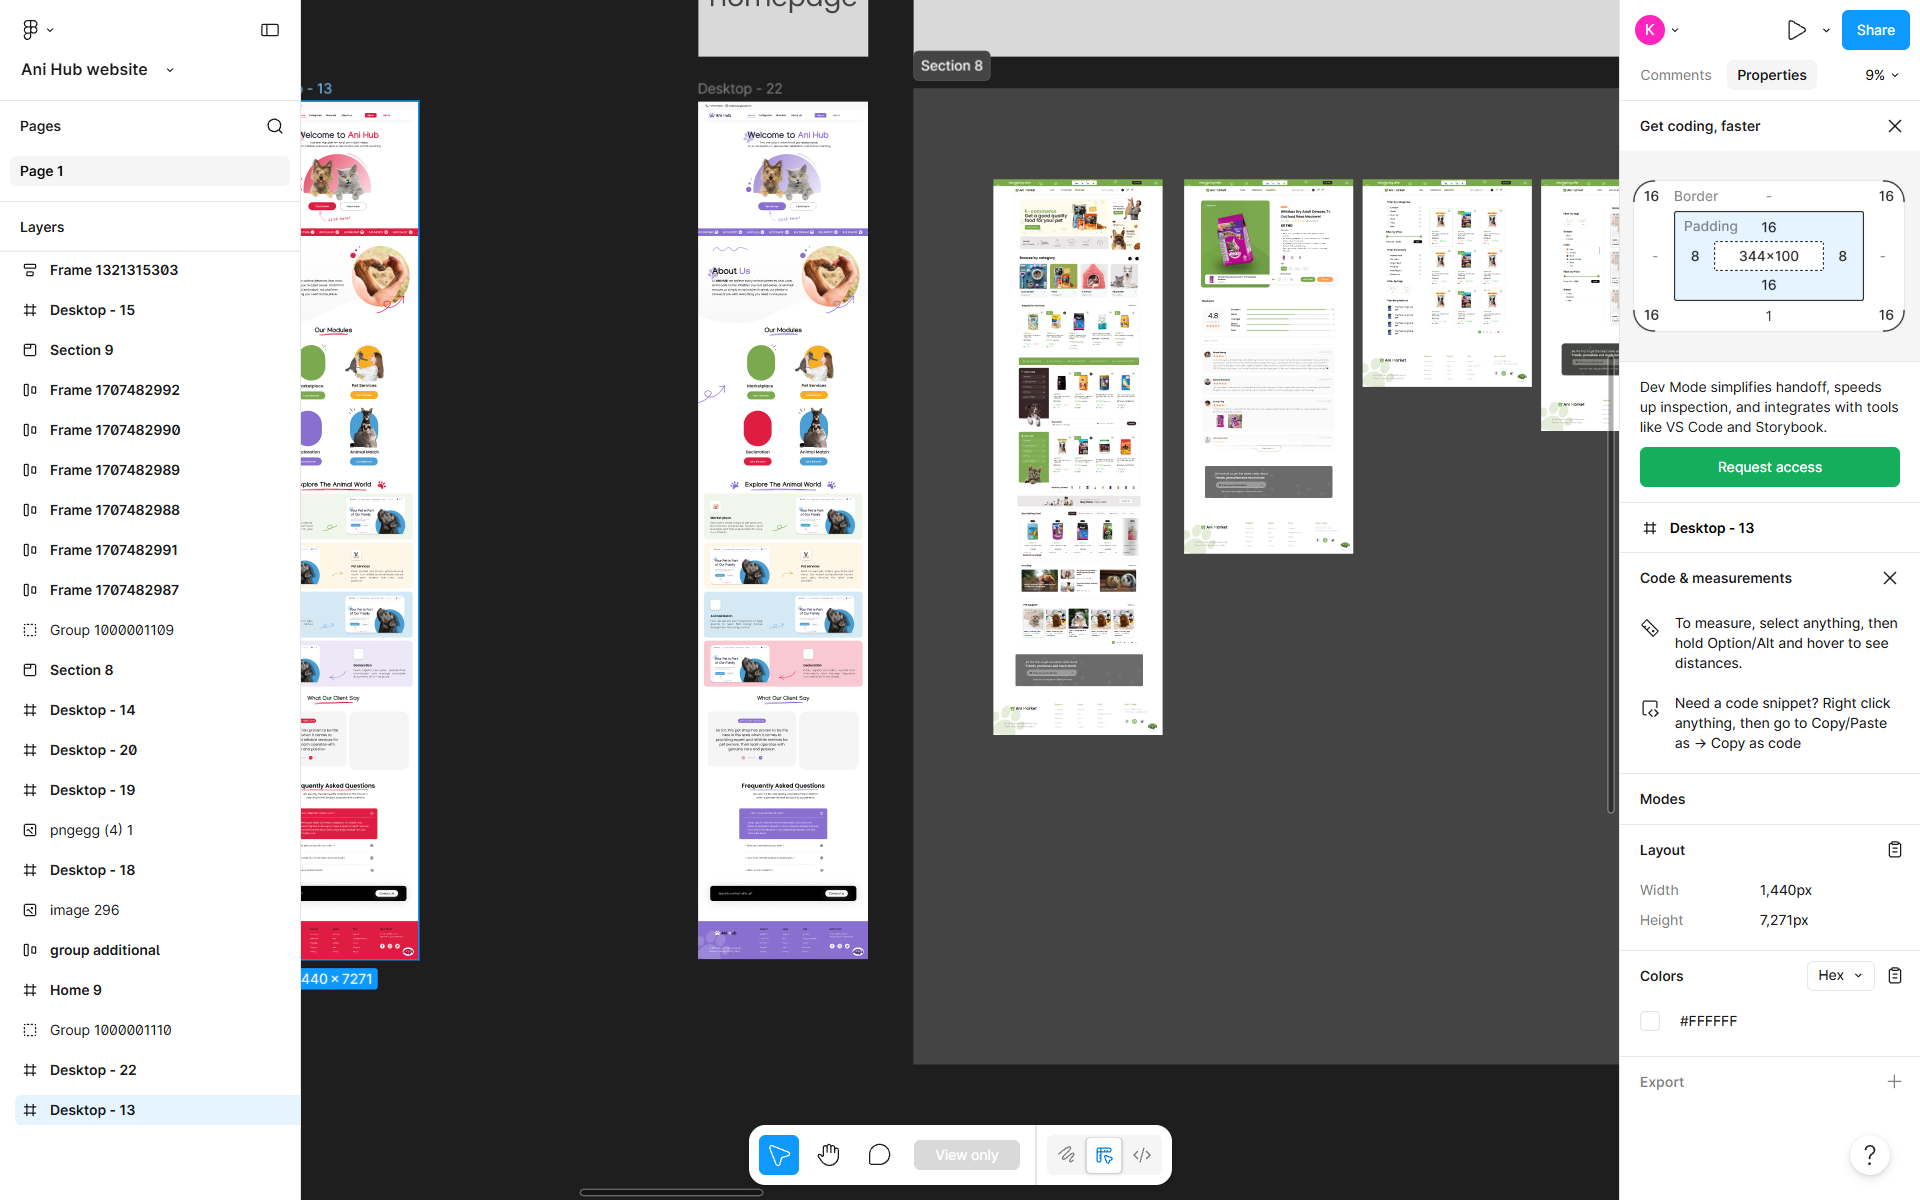
\includegraphics[width=0.64\textwidth]{images/maquettes figma.png}
    \caption{Maquettes Figma des interfaces AniHub}
    \label{fig:figma_maquettes}
\end{figure}


\subsubsection{Page d’accueil AniHub}

La figure \ref{fig:home_anihub} présente la page d’accueil de la plateforme AniHub :

\begin{figure}[h!]
    \centering
    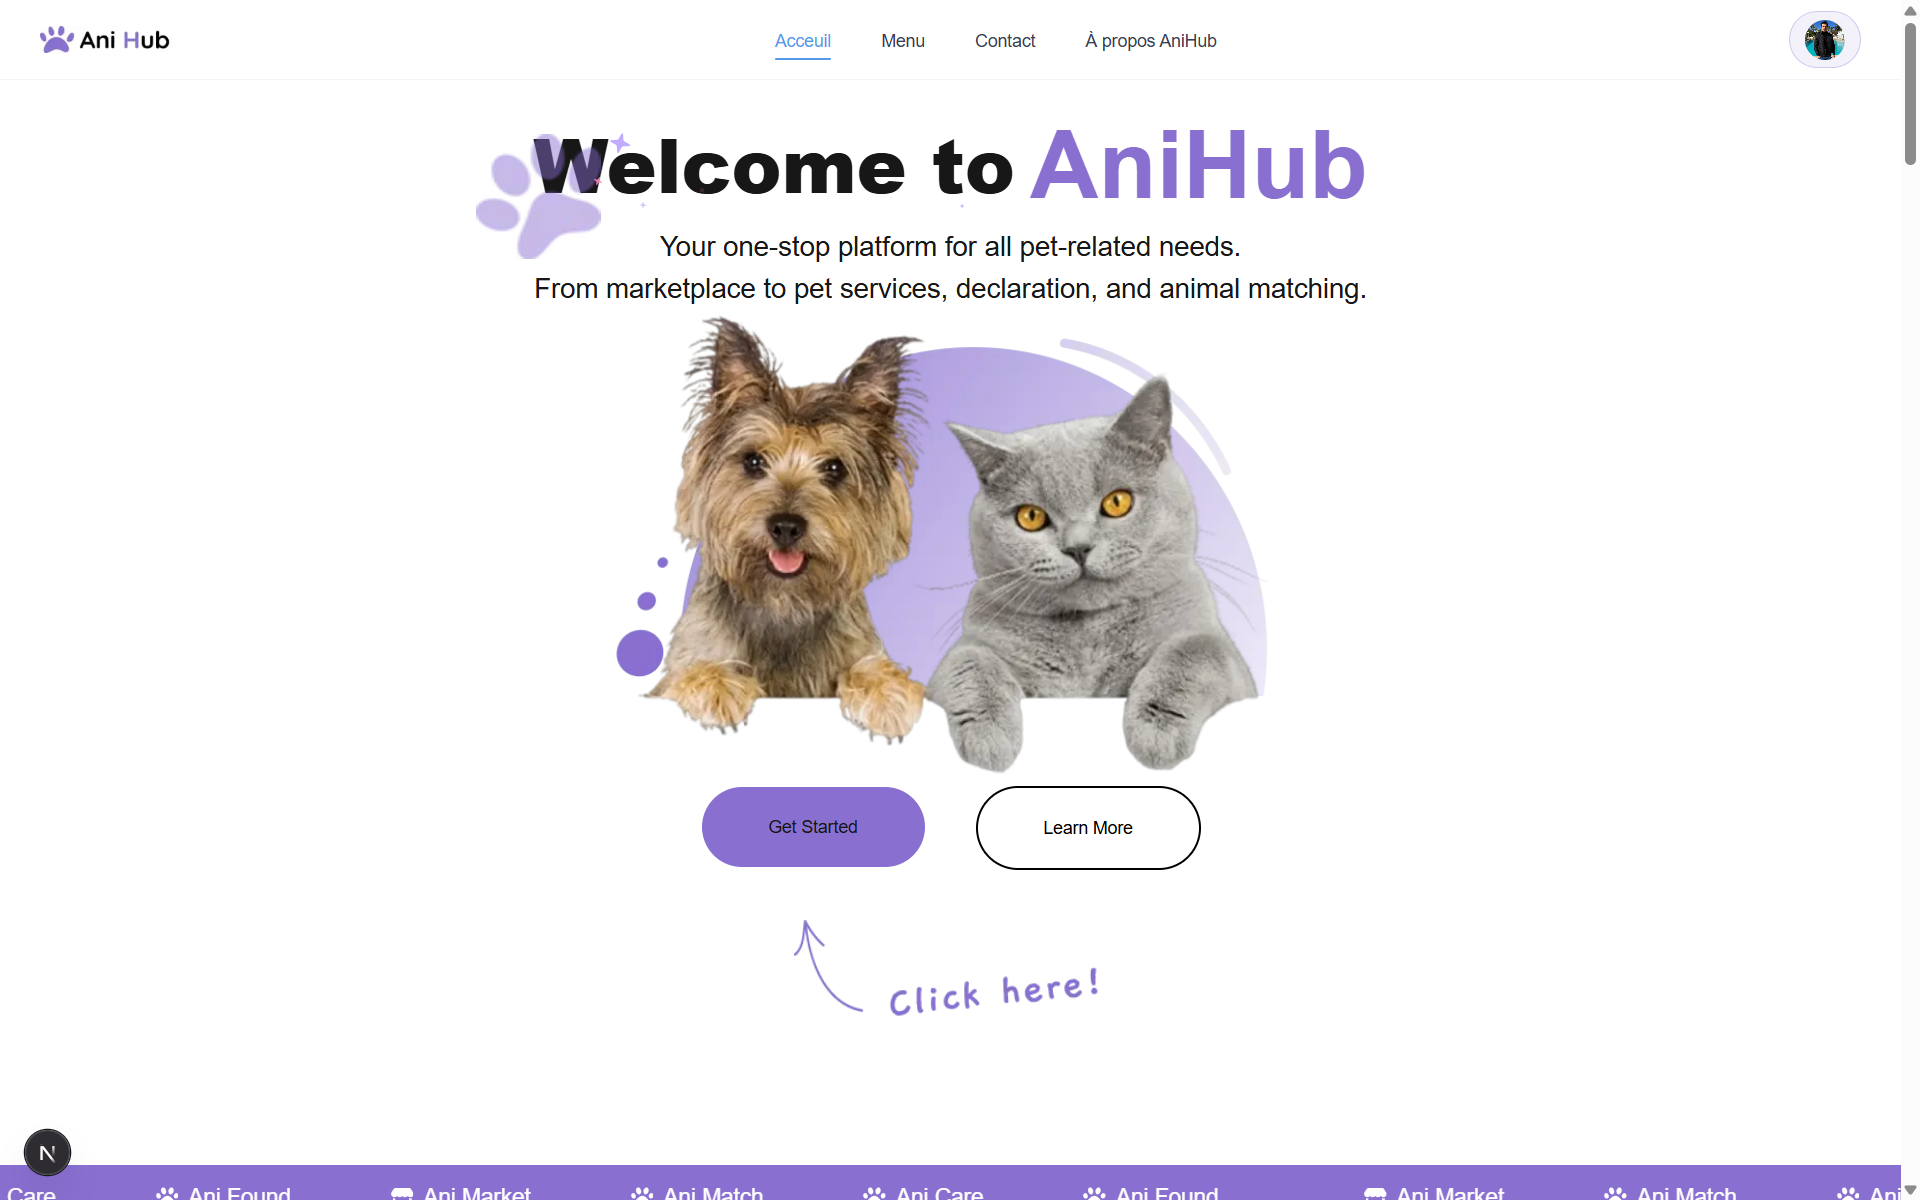
\includegraphics[width=0.72\textwidth]{images/acceuil.png}
    \caption{Page d’accueil AniHub}
    \label{fig:home_anihub}
\end{figure}

\subsubsection{Interfaces d'inscription et de connexion}

Les figures \ref{fig:signup_anihub} et \ref{fig:signin_anihub} illustrent les interfaces d’inscription et de connexion de la plateforme AniHub, qui permettent respectivement la création de compte et l’authentification des utilisateurs : 
\begin{figure}[h!]
    \centering

    \begin{minipage}{0.48\textwidth}
        \centering
        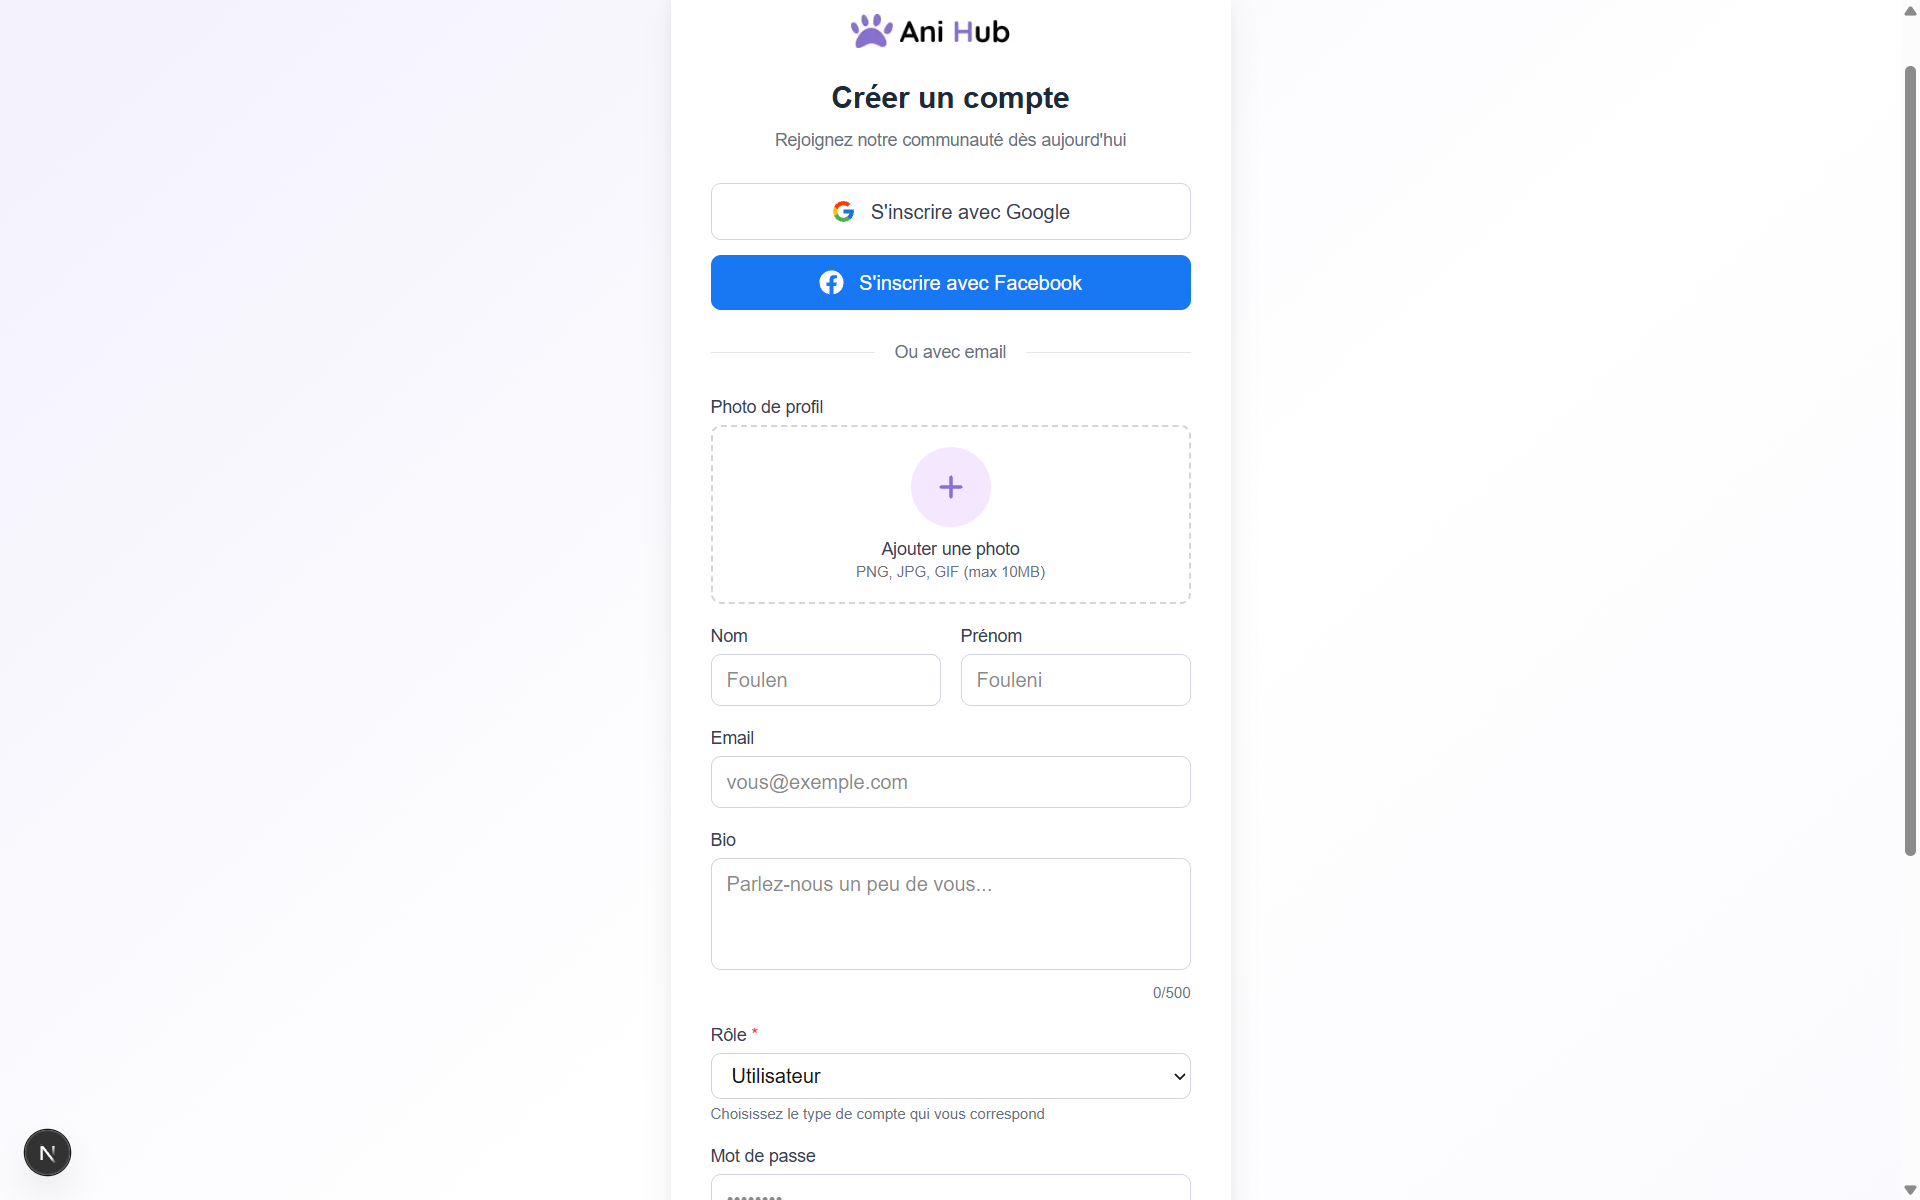
\includegraphics[width=\textwidth]{images/sign up .png}
        \caption{Interface d'inscription AniHub}
        \label{fig:signup_anihub}
    \end{minipage}
    \hfill
    \begin{minipage}{0.48\textwidth}
        \centering
        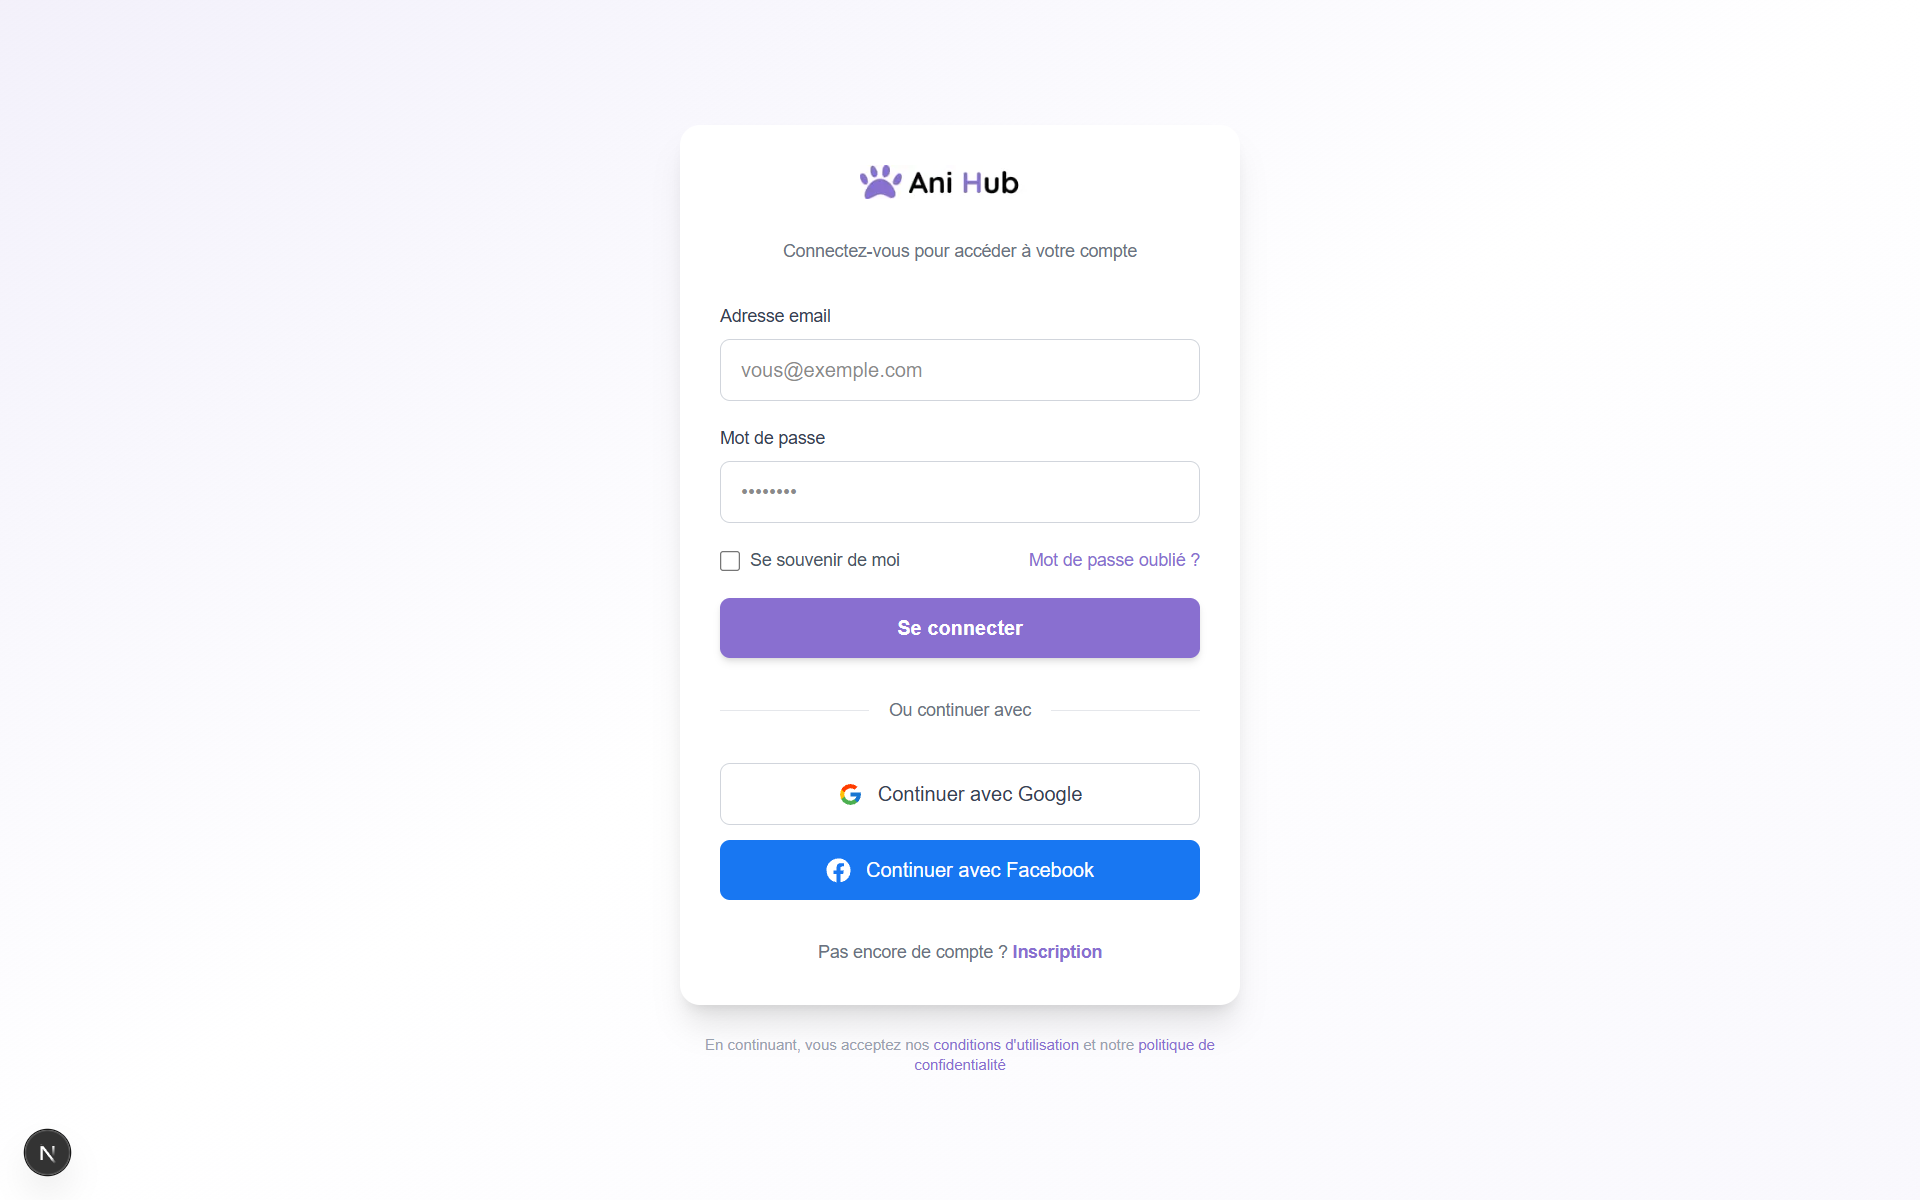
\includegraphics[width=\textwidth]{images/sign in.png}
        \caption{Interface de connexion AniHub}
        \label{fig:signin_anihub}
    \end{minipage}

\end{figure}

\subsubsection{Interface du profil utilisateur}

La figure \ref{fig:profile_anihub} présente l’interface du profil utilisateur AniHub, qui permet à l’utilisateur de consulter et de gérer ses informations personnelles : 
\begin{figure}[H]
    \centering
    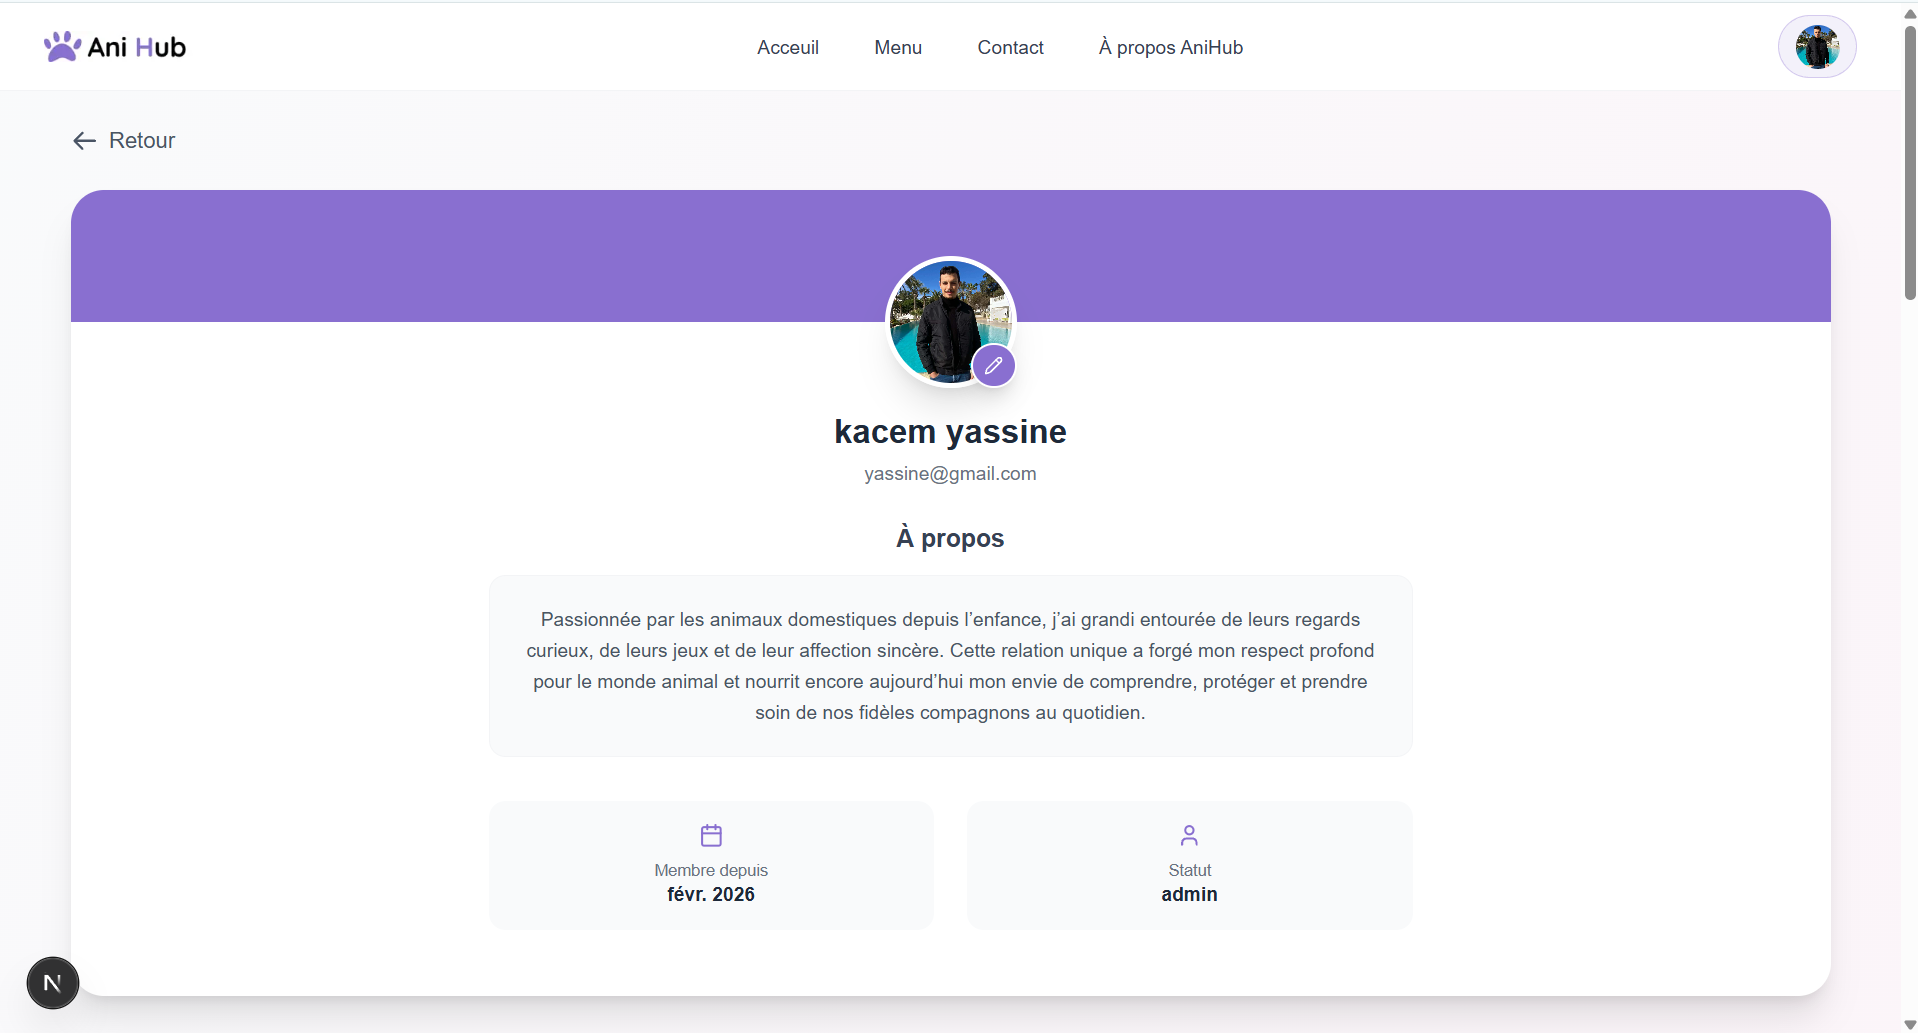
\includegraphics[width=\textwidth]{images/gestion profil.png}
    \caption{Interface du profil utilisateur AniHub}
    \label{fig:profile_anihub}
\end{figure}

\newpage 

\subsubsection{Interface du tableau de bord administrateur}

La figure \ref{fig:admin_dashboard} présente l’accueil du tableau de bord administrateur de la plateforme AniHub, qui affiche des statistiques globales sur la plateforme : 
\begin{figure}[H]
    \centering
    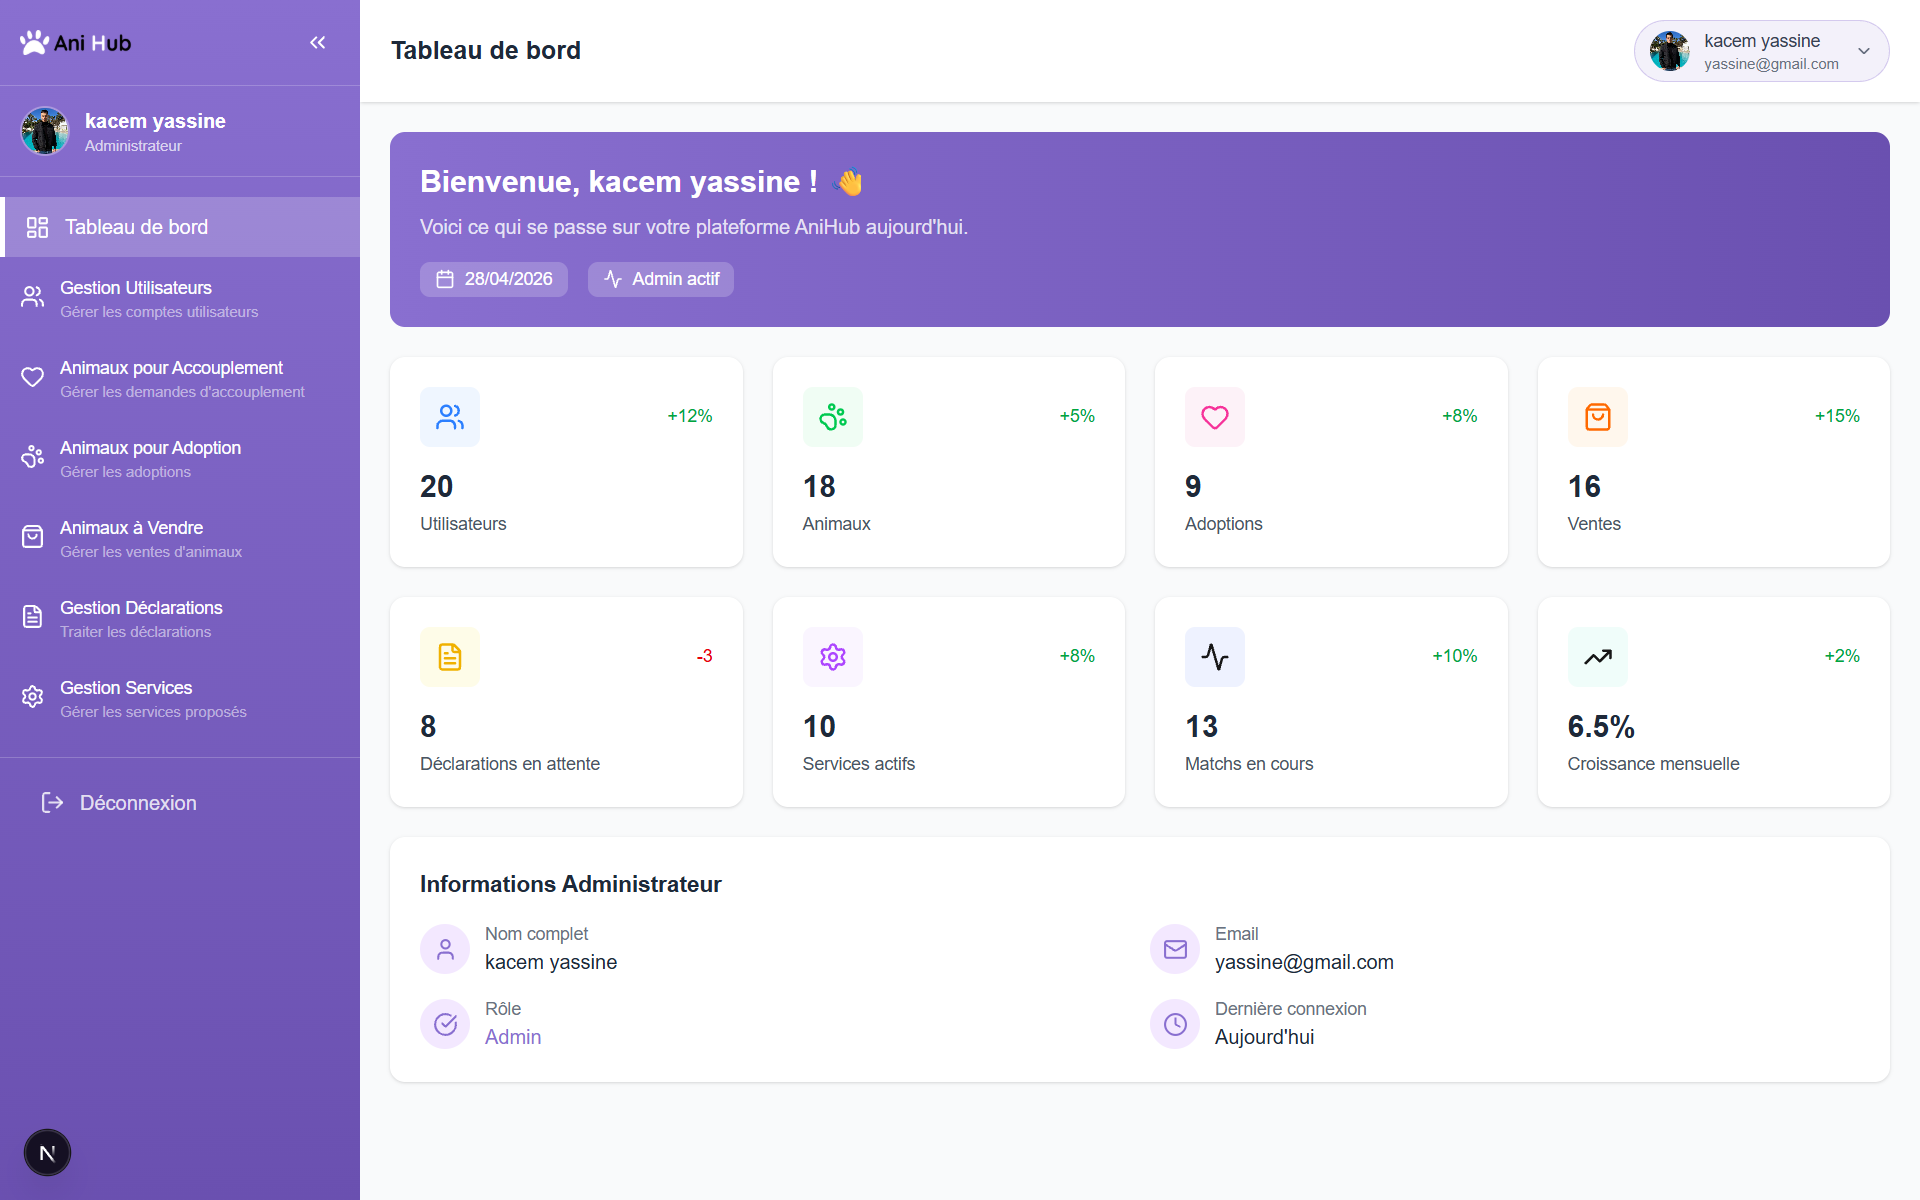
\includegraphics[width=0.75\textwidth]{images/dashboard stats.png}
    \caption{Tableau de bord administrateur AniHub}
    \label{fig:admin_dashboard}
\end{figure}

\subsubsection{Interface de gestion des utilisateurs}

La figure \ref{fig:user_management} présente l’interface de gestion des utilisateurs de la plateforme AniHub : 

\begin{figure}[H]
    \centering
    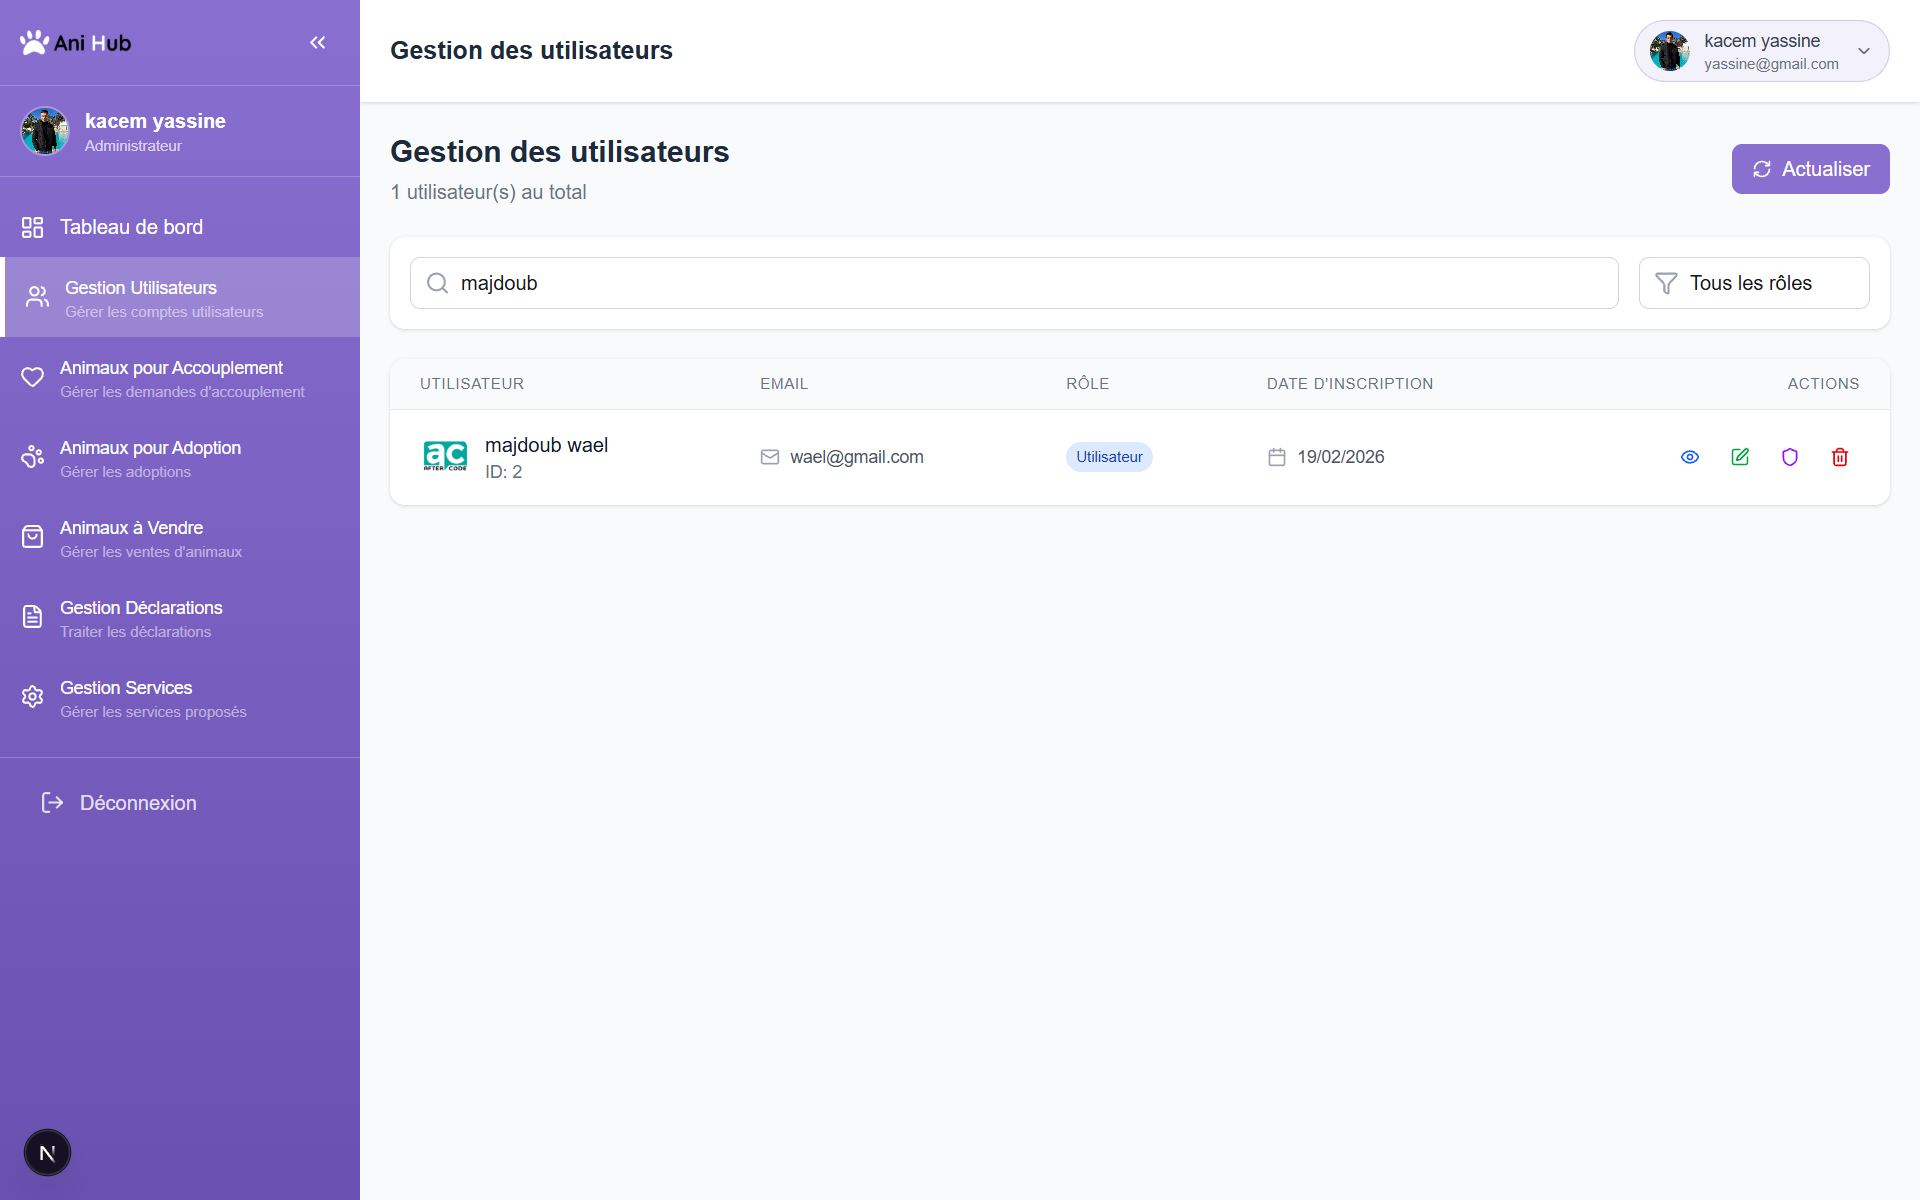
\includegraphics[width=0.78\textwidth]{images/gestion utilsateurs.png}
    \caption{Interface de gestion des utilisateurs AniHub}
    \label{fig:user_management}
\end{figure}

\newpage

\subsubsection{Interfaces d’administration pour le module AniMatch avec statistiques} 

Les figures \ref{fig:animatch_manage} et \ref{fig:animatch_stats} illustrent les interfaces permettant à l’administrateur de gérer le module AniMatch (accouplement et adoption ) et de consulter les statistiques associées, notamment le suivi des demandes de mise en relation, leur validation ainsi que l’analyse de l’activité des utilisateurs au sein de ce module : 
\begin{figure}[h!]
    \centering
    
    \begin{minipage}{0.48\textwidth}
        \centering
        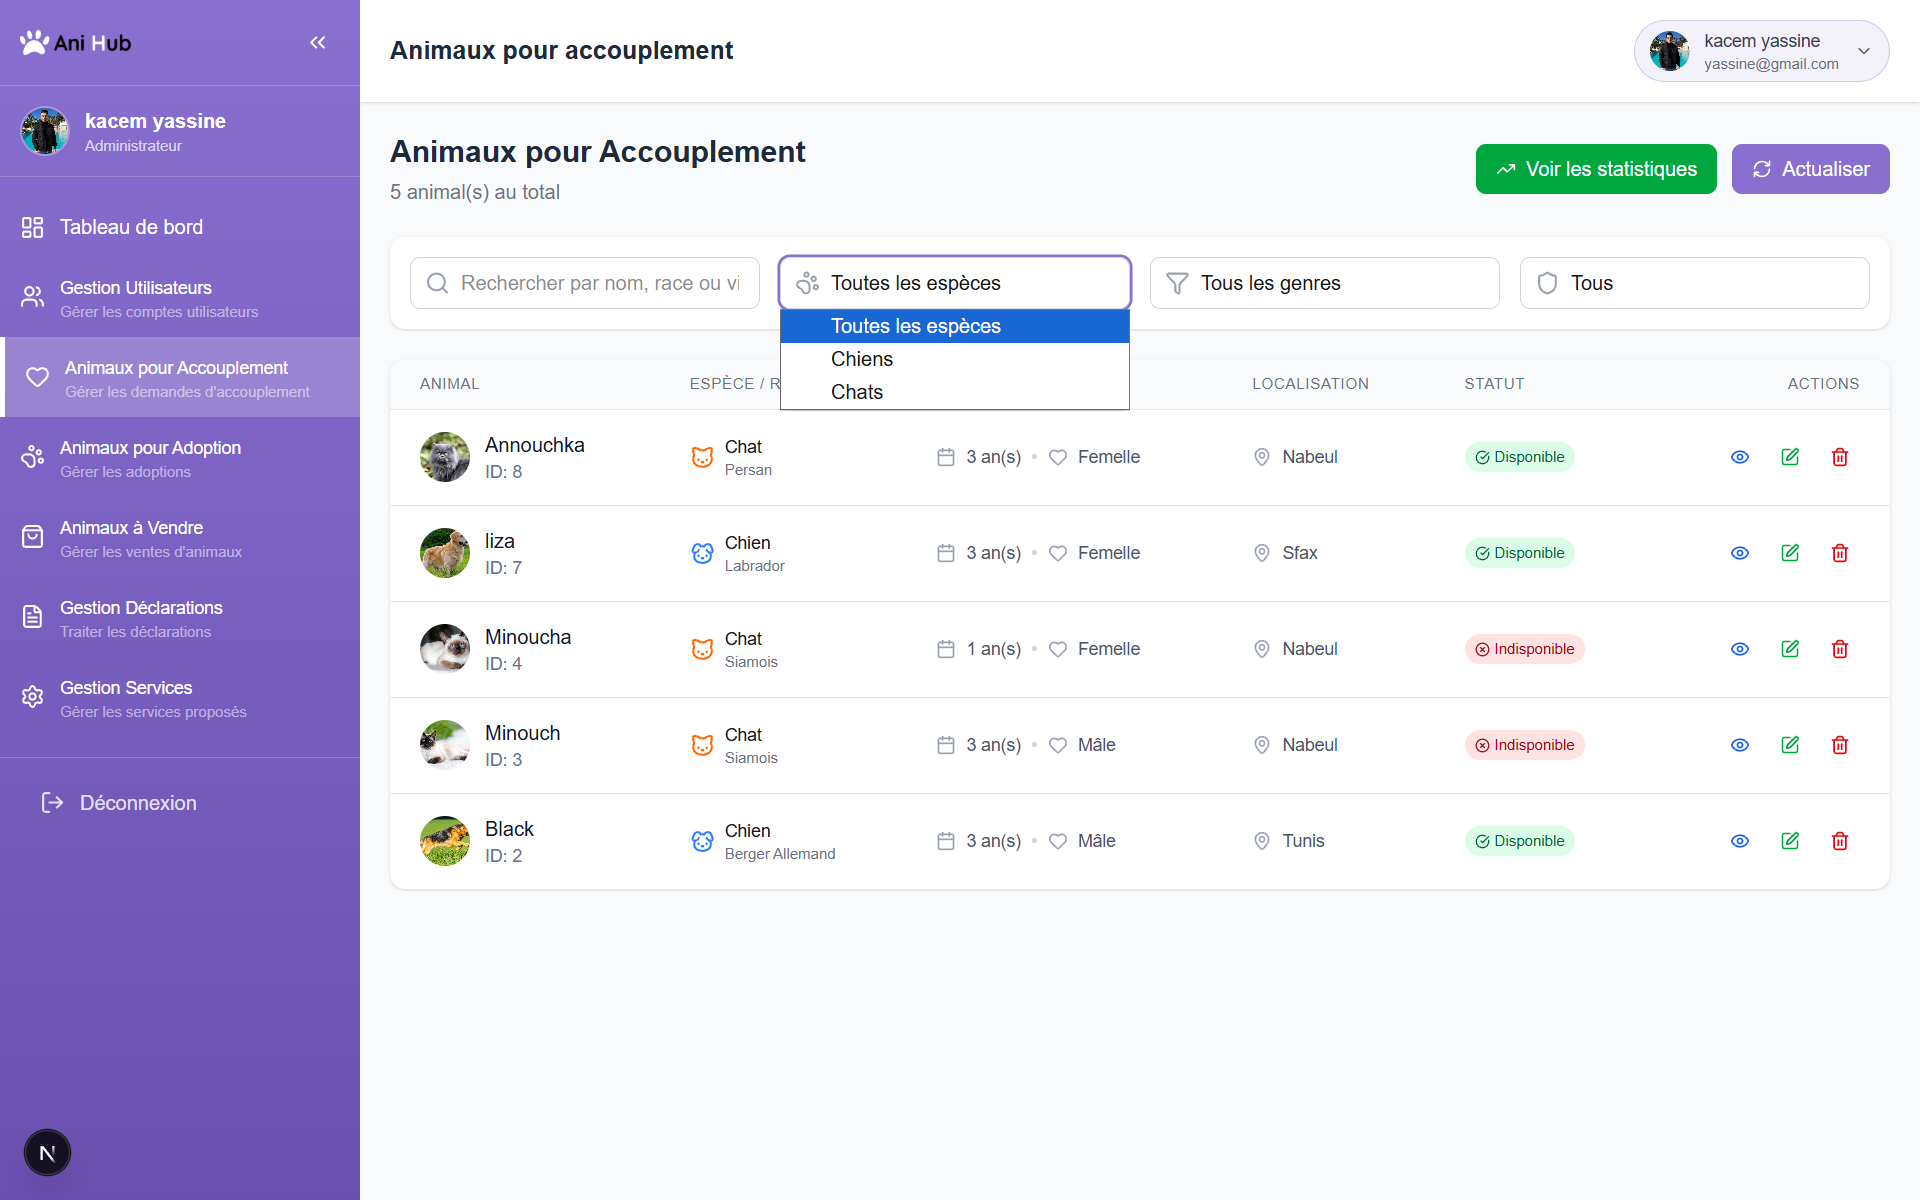
\includegraphics[width=\textwidth]{images/dashboard animatch 1.png}
        \caption{Interface d’administration de gestion d’AniMatch}
        \label{fig:animatch_manage}
    \end{minipage}
    \hfill
    \begin{minipage}{0.48\textwidth}
        \centering
        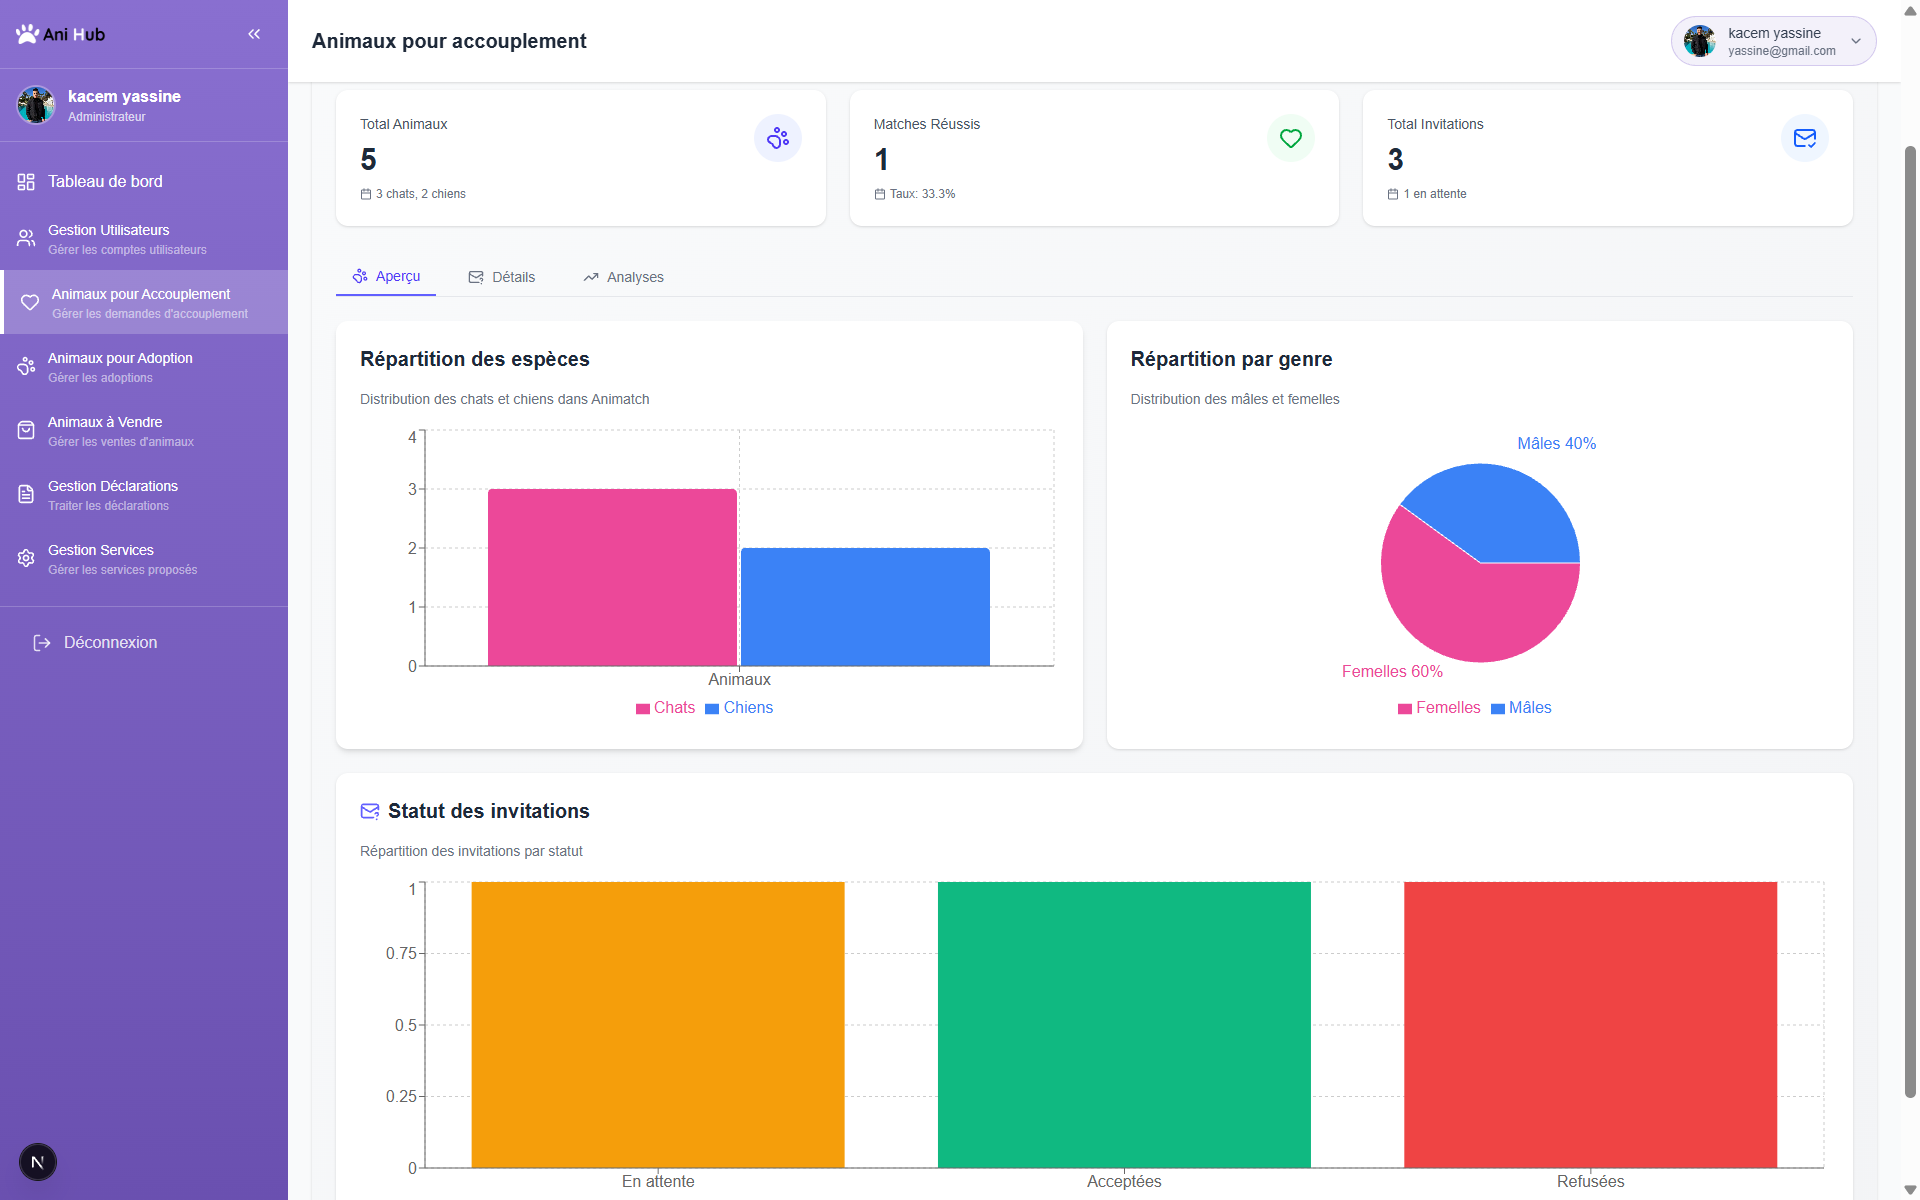
\includegraphics[width=\textwidth]{images/dashboard animatch 2.png}
        \caption{Interface d’administration des statistiques d’AniMatch}
        \label{fig:animatch_stats}
    \end{minipage}

\end{figure}

\subsubsection{Interfaces d’administration pour le module AniFound avec statistiques}  

Les figures \ref{fig:anifound_manage} et \ref{fig:anifound_stats} illustrent les interfaces permettant à l’administrateur de gérer le module AniFound, dédié au signalement des animaux perdus et trouvés, ainsi que de consulter les statistiques associées afin de suivre l’activité et les publications du module : 
\begin{figure}[h!]
    \centering
    
    \begin{minipage}{0.48\textwidth}
        \centering
        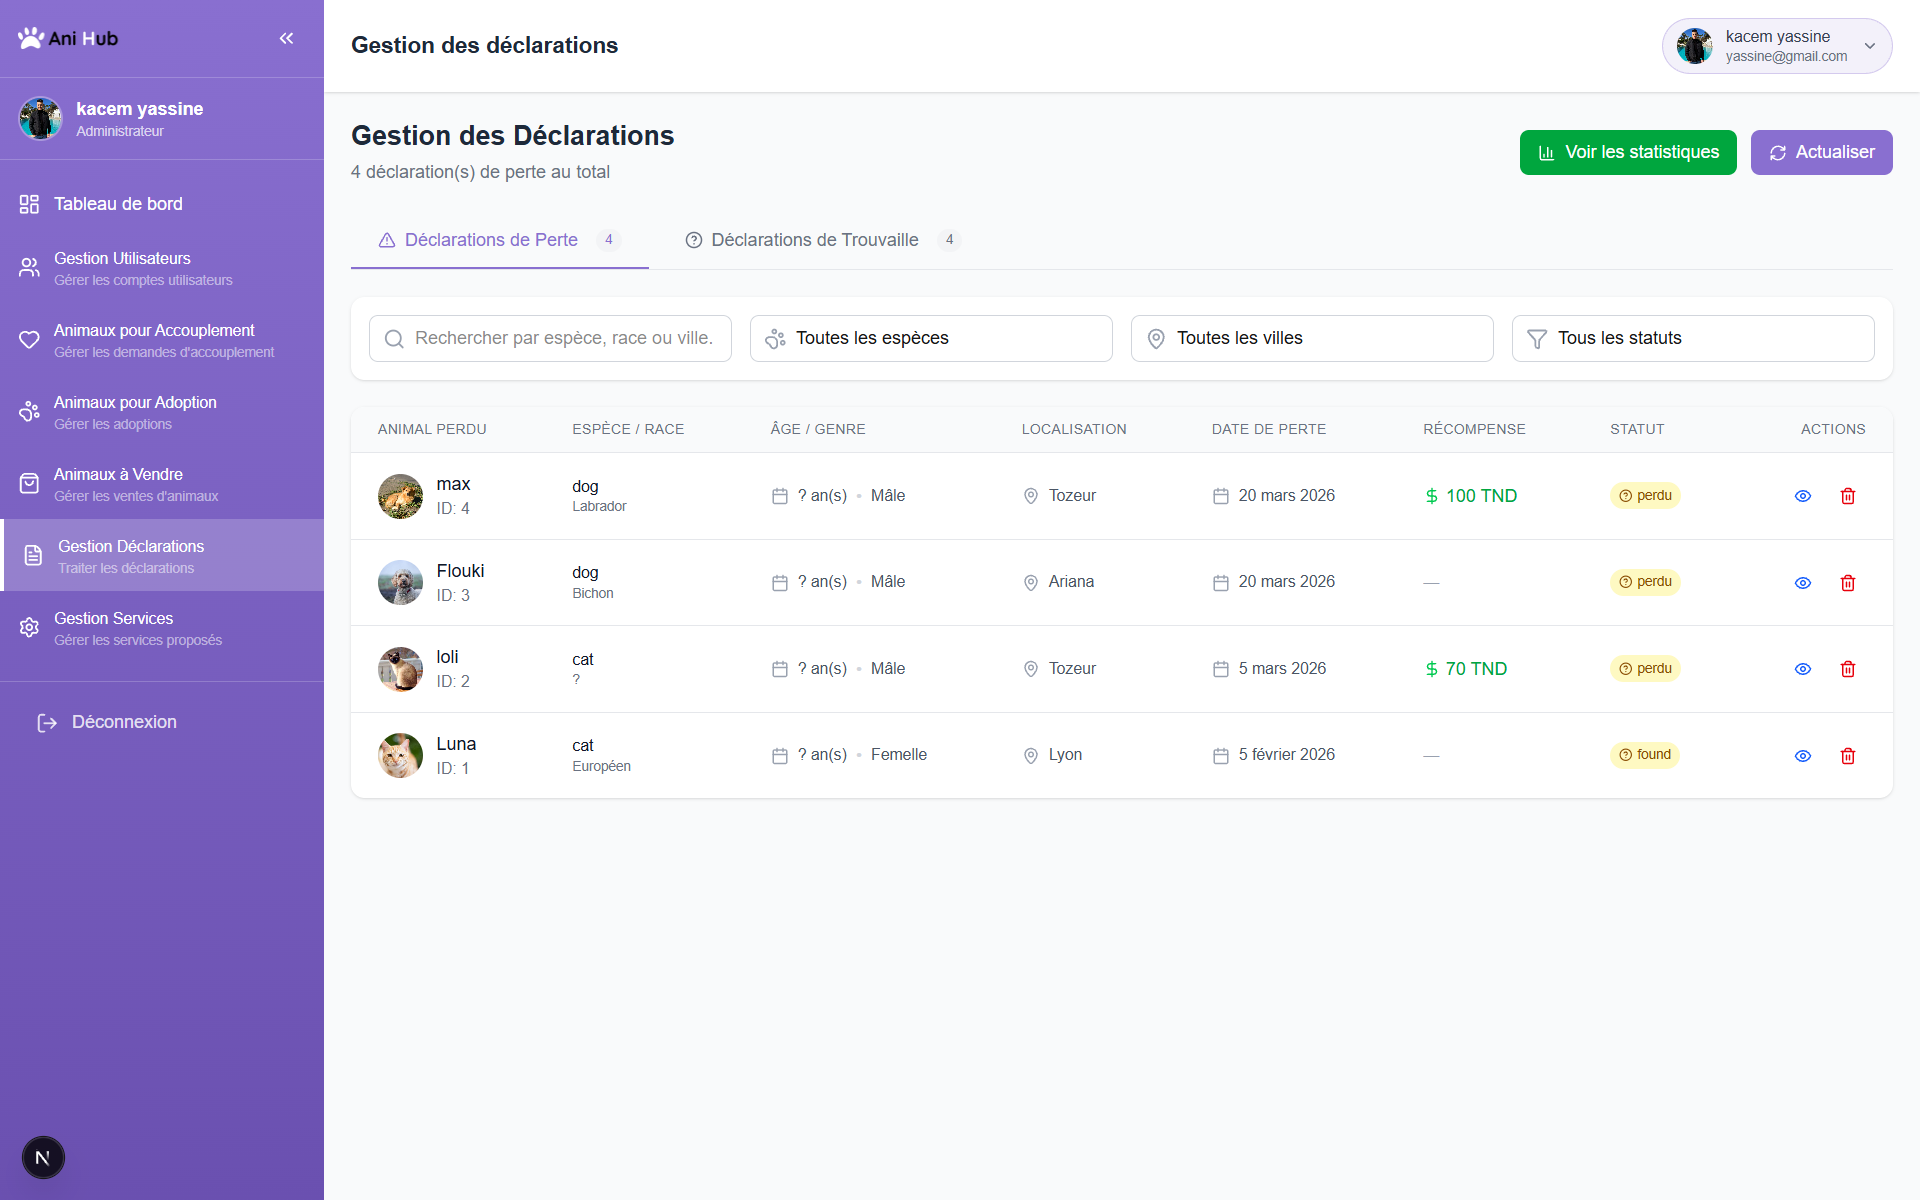
\includegraphics[width=\textwidth]{images/dashboard anifound 1.png}
        \caption{Interface d’administration de gestion d’AniFound}
        \label{fig:anifound_manage}
    \end{minipage}
    \hfill
    \begin{minipage}{0.48\textwidth}
        \centering
        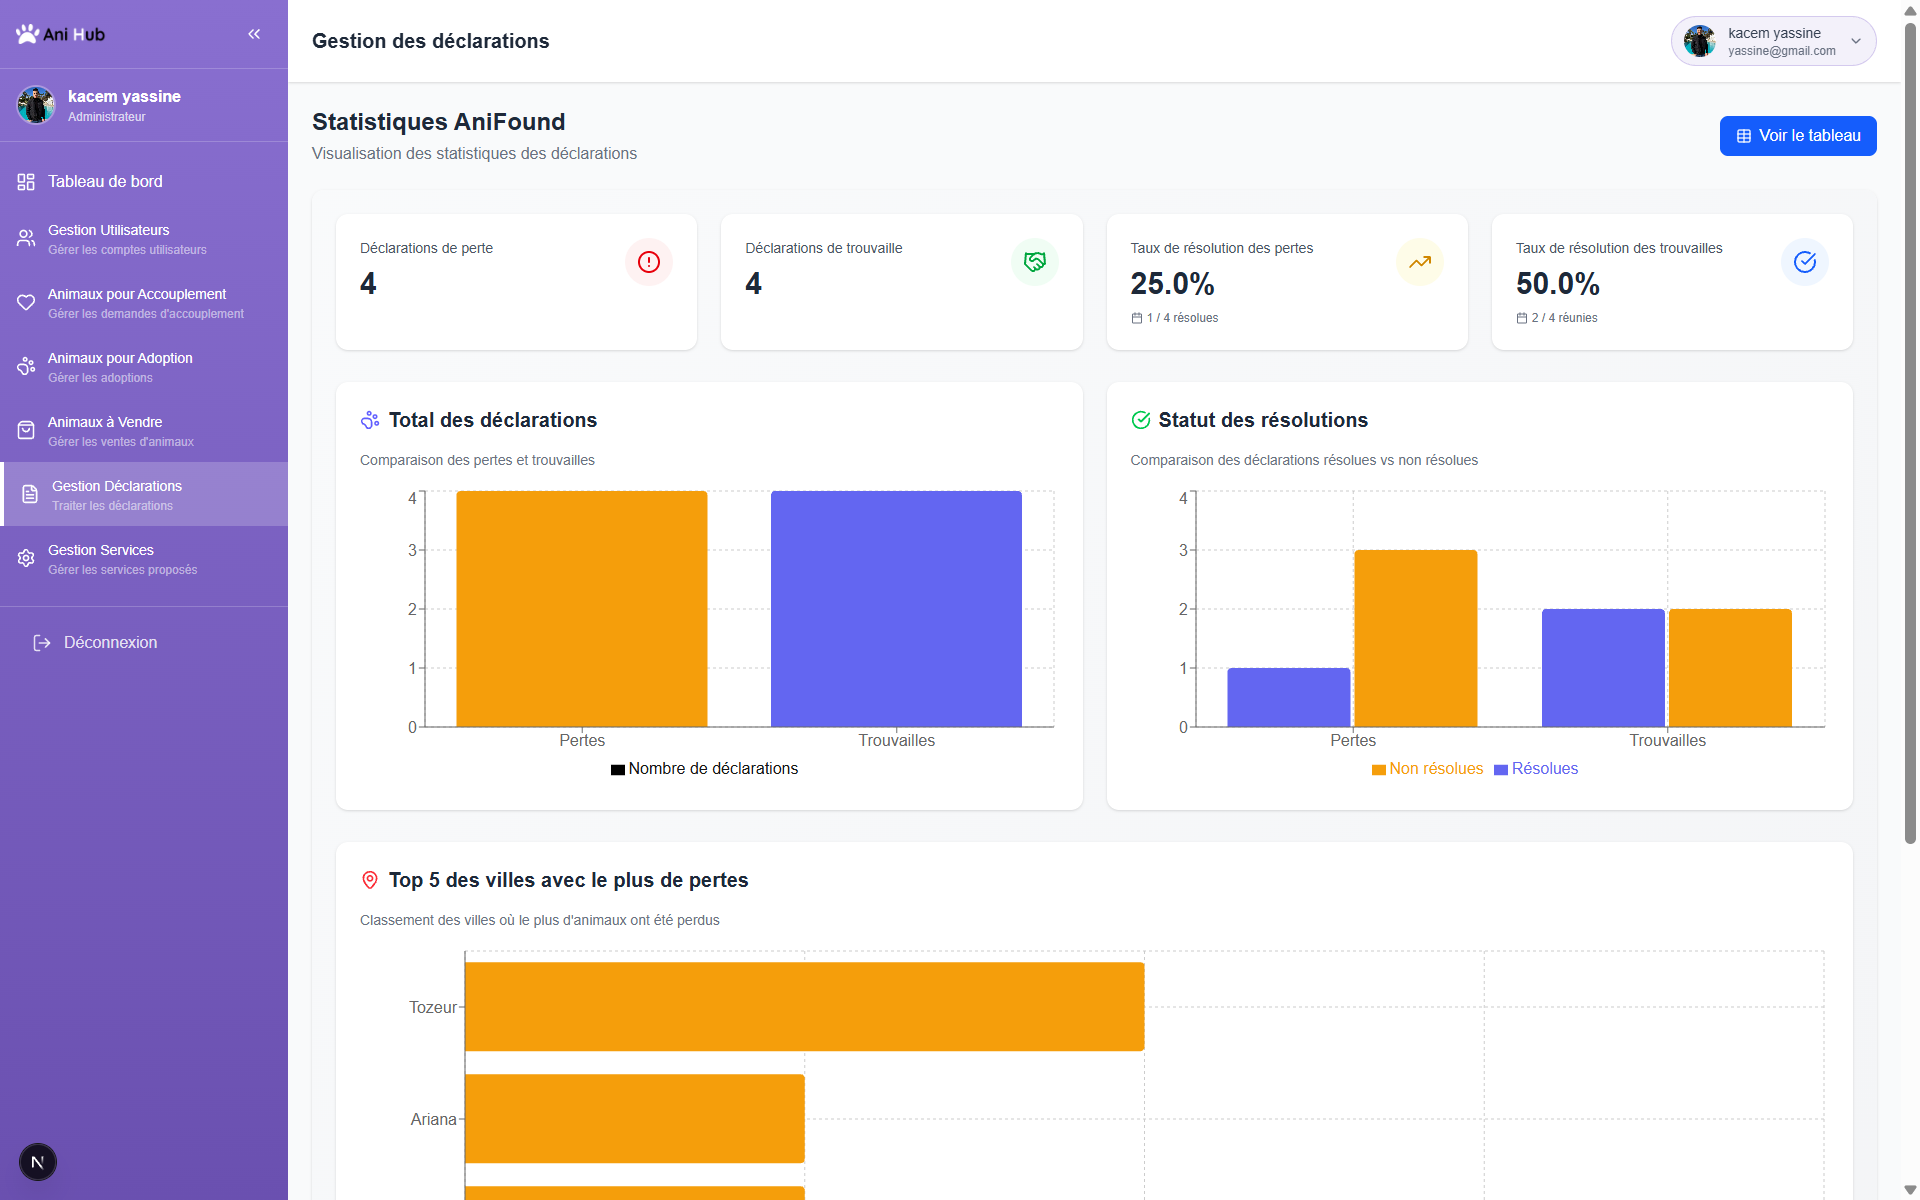
\includegraphics[width=\textwidth]{images/dashboard anifound 2.png}
        \caption{Interface d’administration des statistiques d’AniFound}
        \label{fig:anifound_stats}
    \end{minipage}

\end{figure}

\newpage

\subsubsection{Interfaces d’administration pour le module AniMarket avec statistiques}

Les figures \ref{fig:animarket_manage} et \ref{fig:animarket_stats} illustrent les interfaces permettant à l’administrateur de gérer le module AniMarket (le module de vente, achat et enchères d’animaux en ligne) et de consulter les statistiques associées : 

\begin{figure}[h!]
    \centering

    \begin{minipage}{0.48\textwidth}
        \centering
        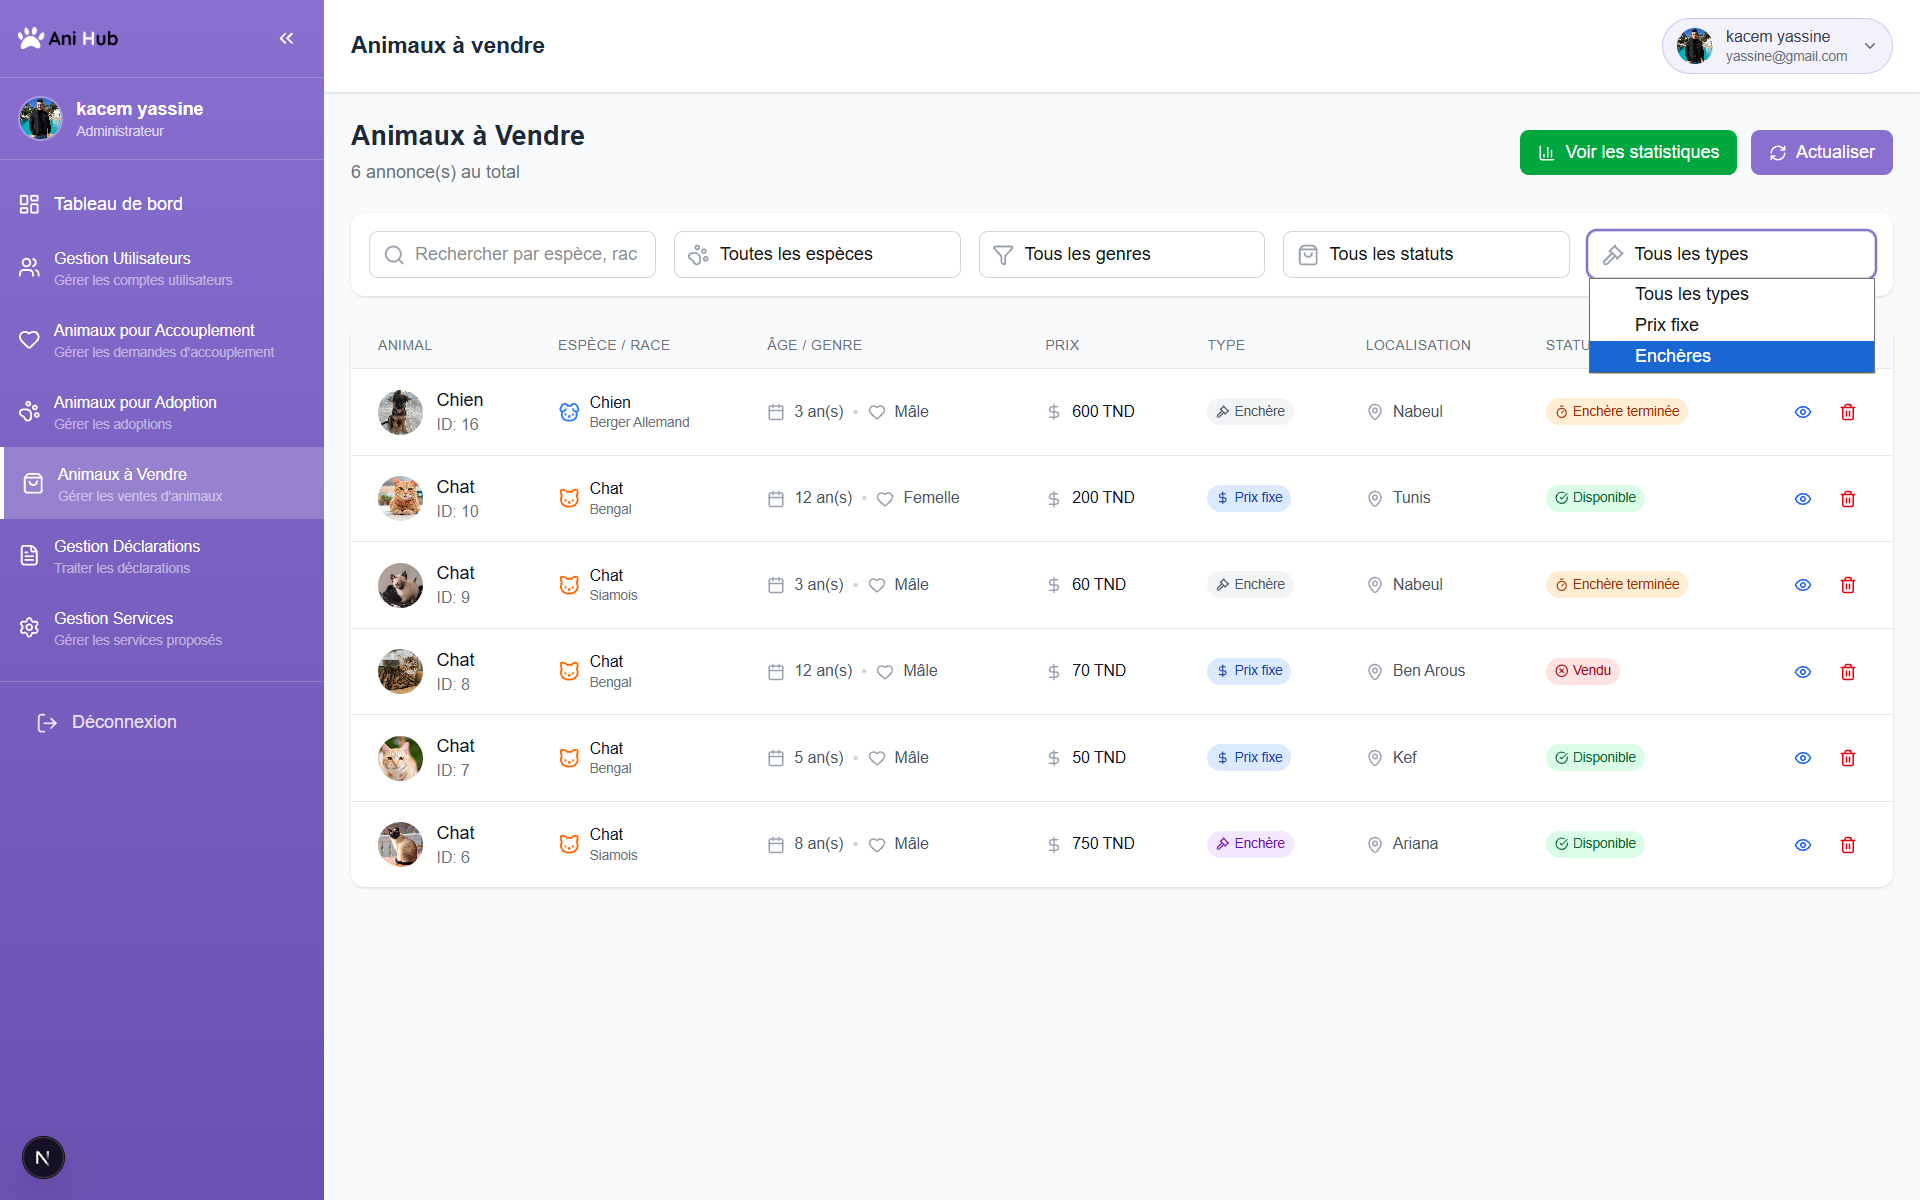
\includegraphics[width=\textwidth]{images/dashboard animarket 1.png}
        \caption{Interface d’administration de gestion d’AniMarket}
        \label{fig:animarket_manage}
    \end{minipage}
    \hfill
    \begin{minipage}{0.48\textwidth}
        \centering
        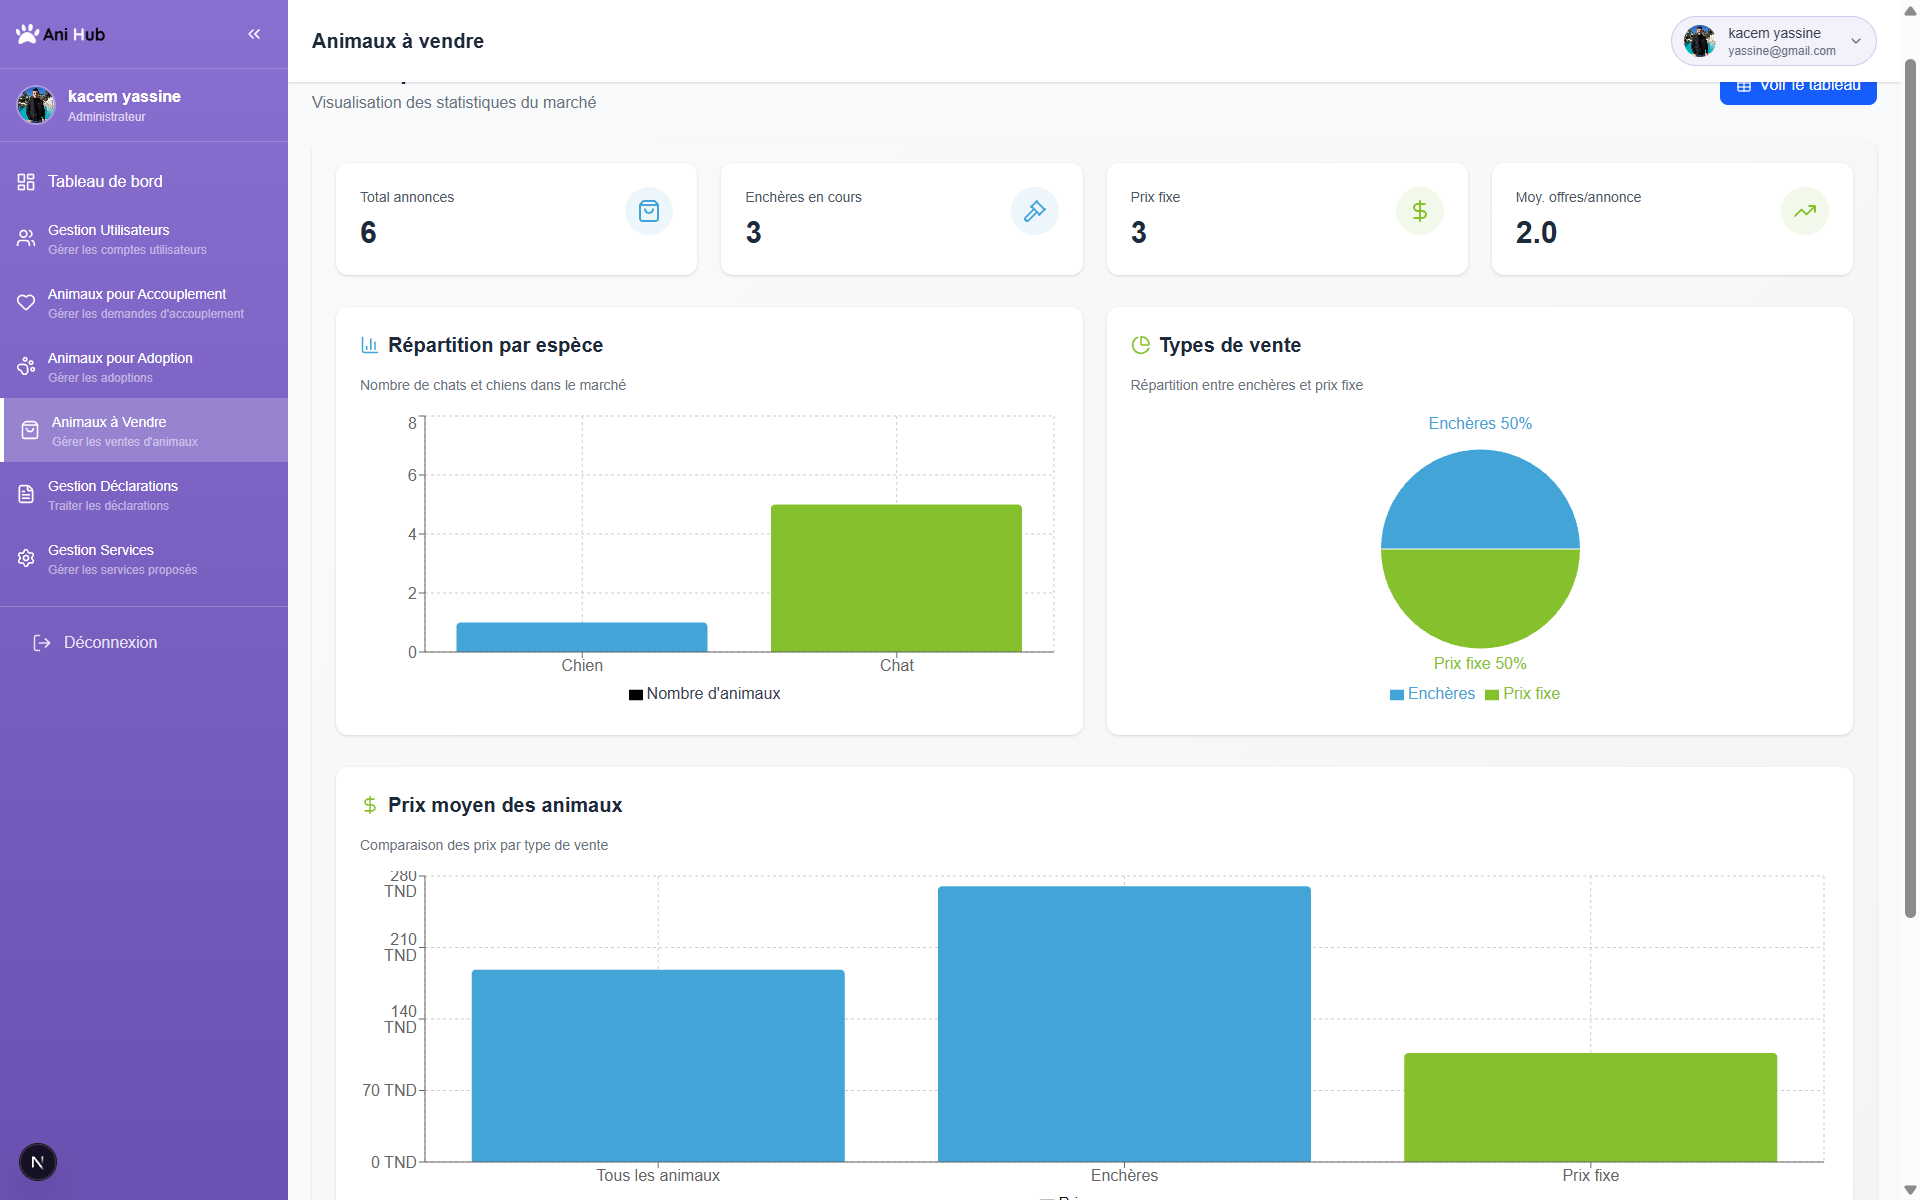
\includegraphics[width=\textwidth]{images/dashboard animarket 2.png}
        \caption{Interface d’administration des statistiques d’AniMarket}
        \label{fig:animarket_stats}
    \end{minipage}

\end{figure}

\subsubsection{Interface d’administration AniCare : gestion des services} 

La figure \ref{fig:anicare_manage} illustre la gestion des services dans le module AniCare, tels que les services de dressage, de soins vétérinaires, de toilettage et de garderie publiés par les prestataires de services : 
\begin{figure}[h!]
    \centering
    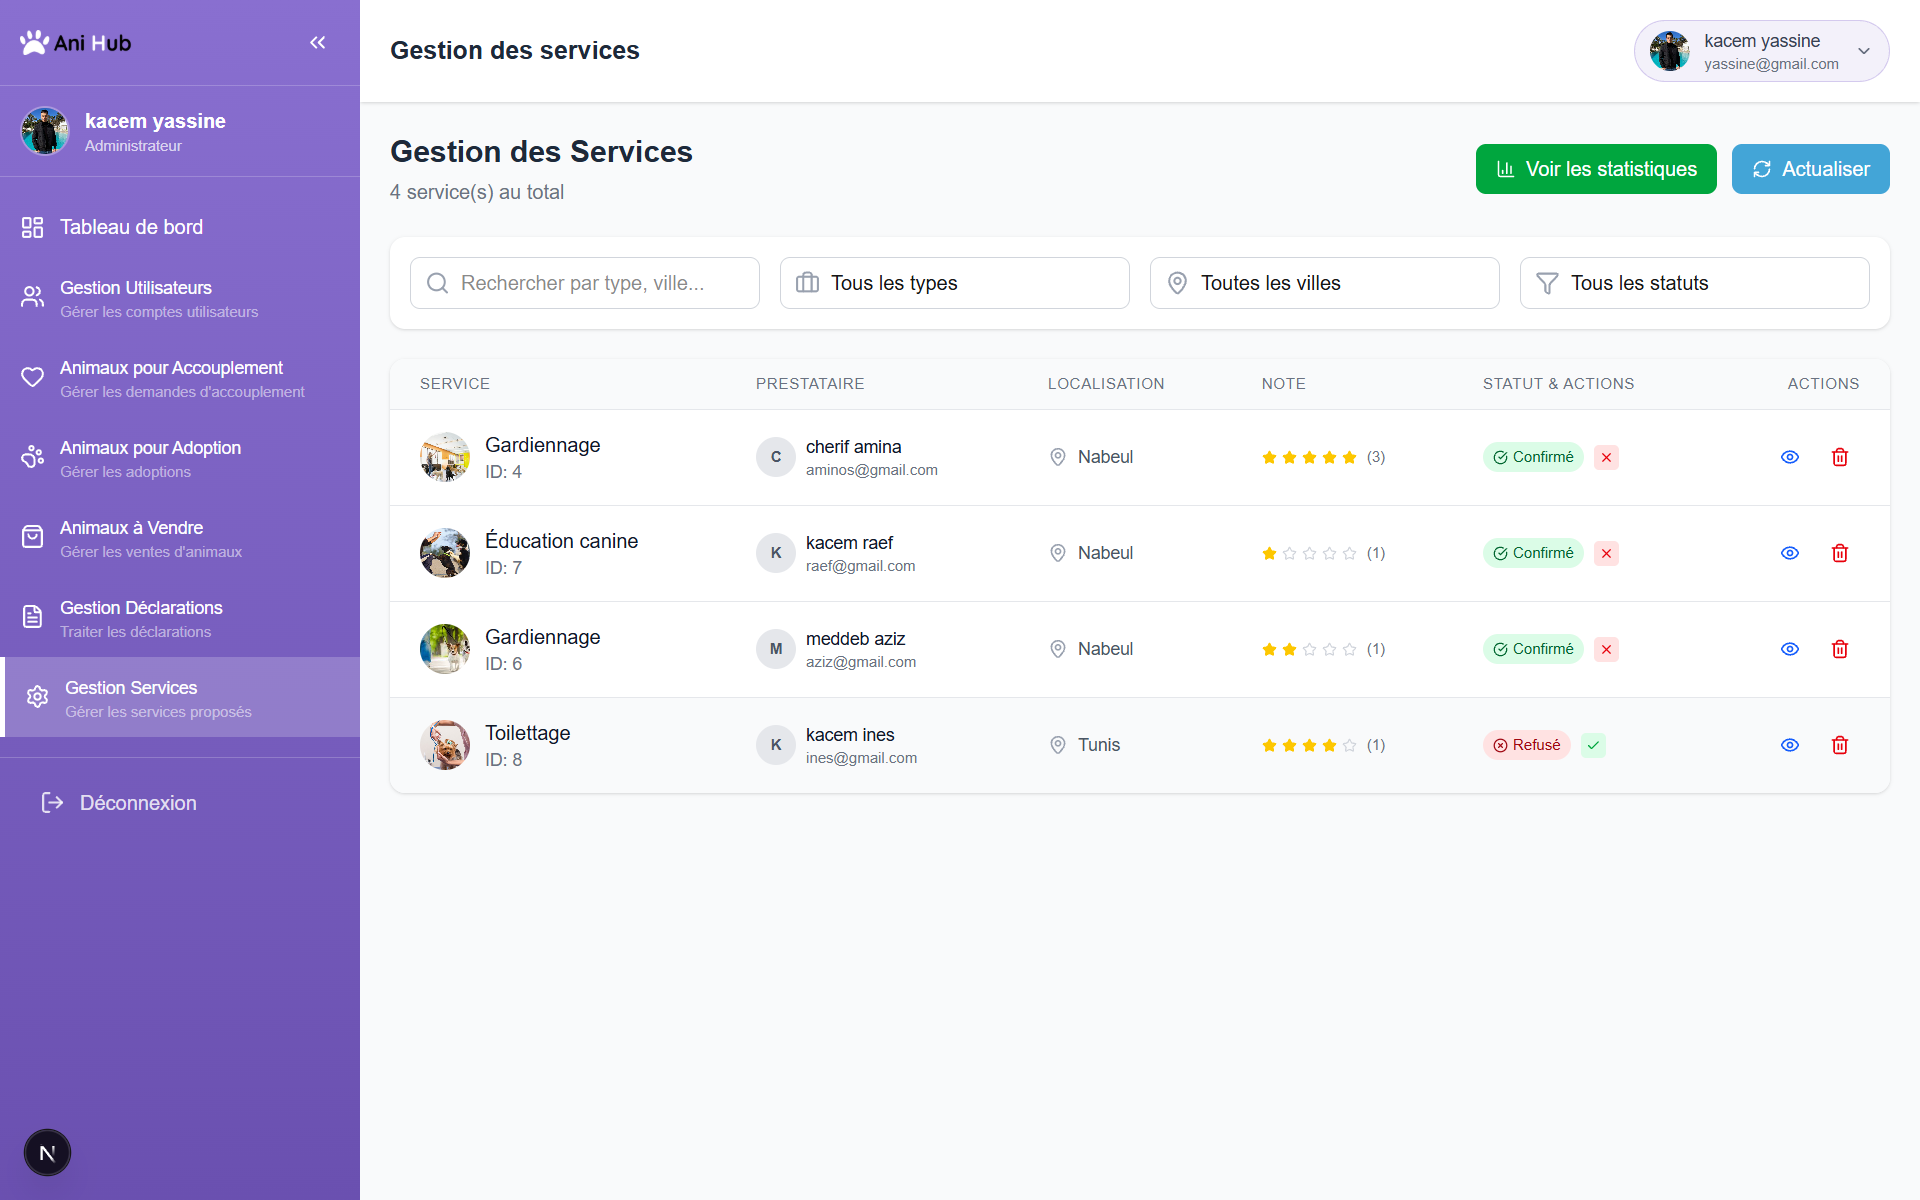
\includegraphics[width=0.8\textwidth]{images/dashboard anicare 1.png}
    \caption{Interface d’administration AniCare : gestion des services}
    \label{fig:anicare_manage}
\end{figure}

\newpage 

\subsubsection{Interface d’administration AniCare : vérification des services} 

La figure \ref{fig:anicare_verify} illustre l’interface de vérification des services dans le module AniCare, qui permet à l’administrateur de vérifier les documents justificatifs fournis par les prestataires de services avant de confirmer leurs services sur la plateforme : 
\begin{figure}[h!]
    \centering
    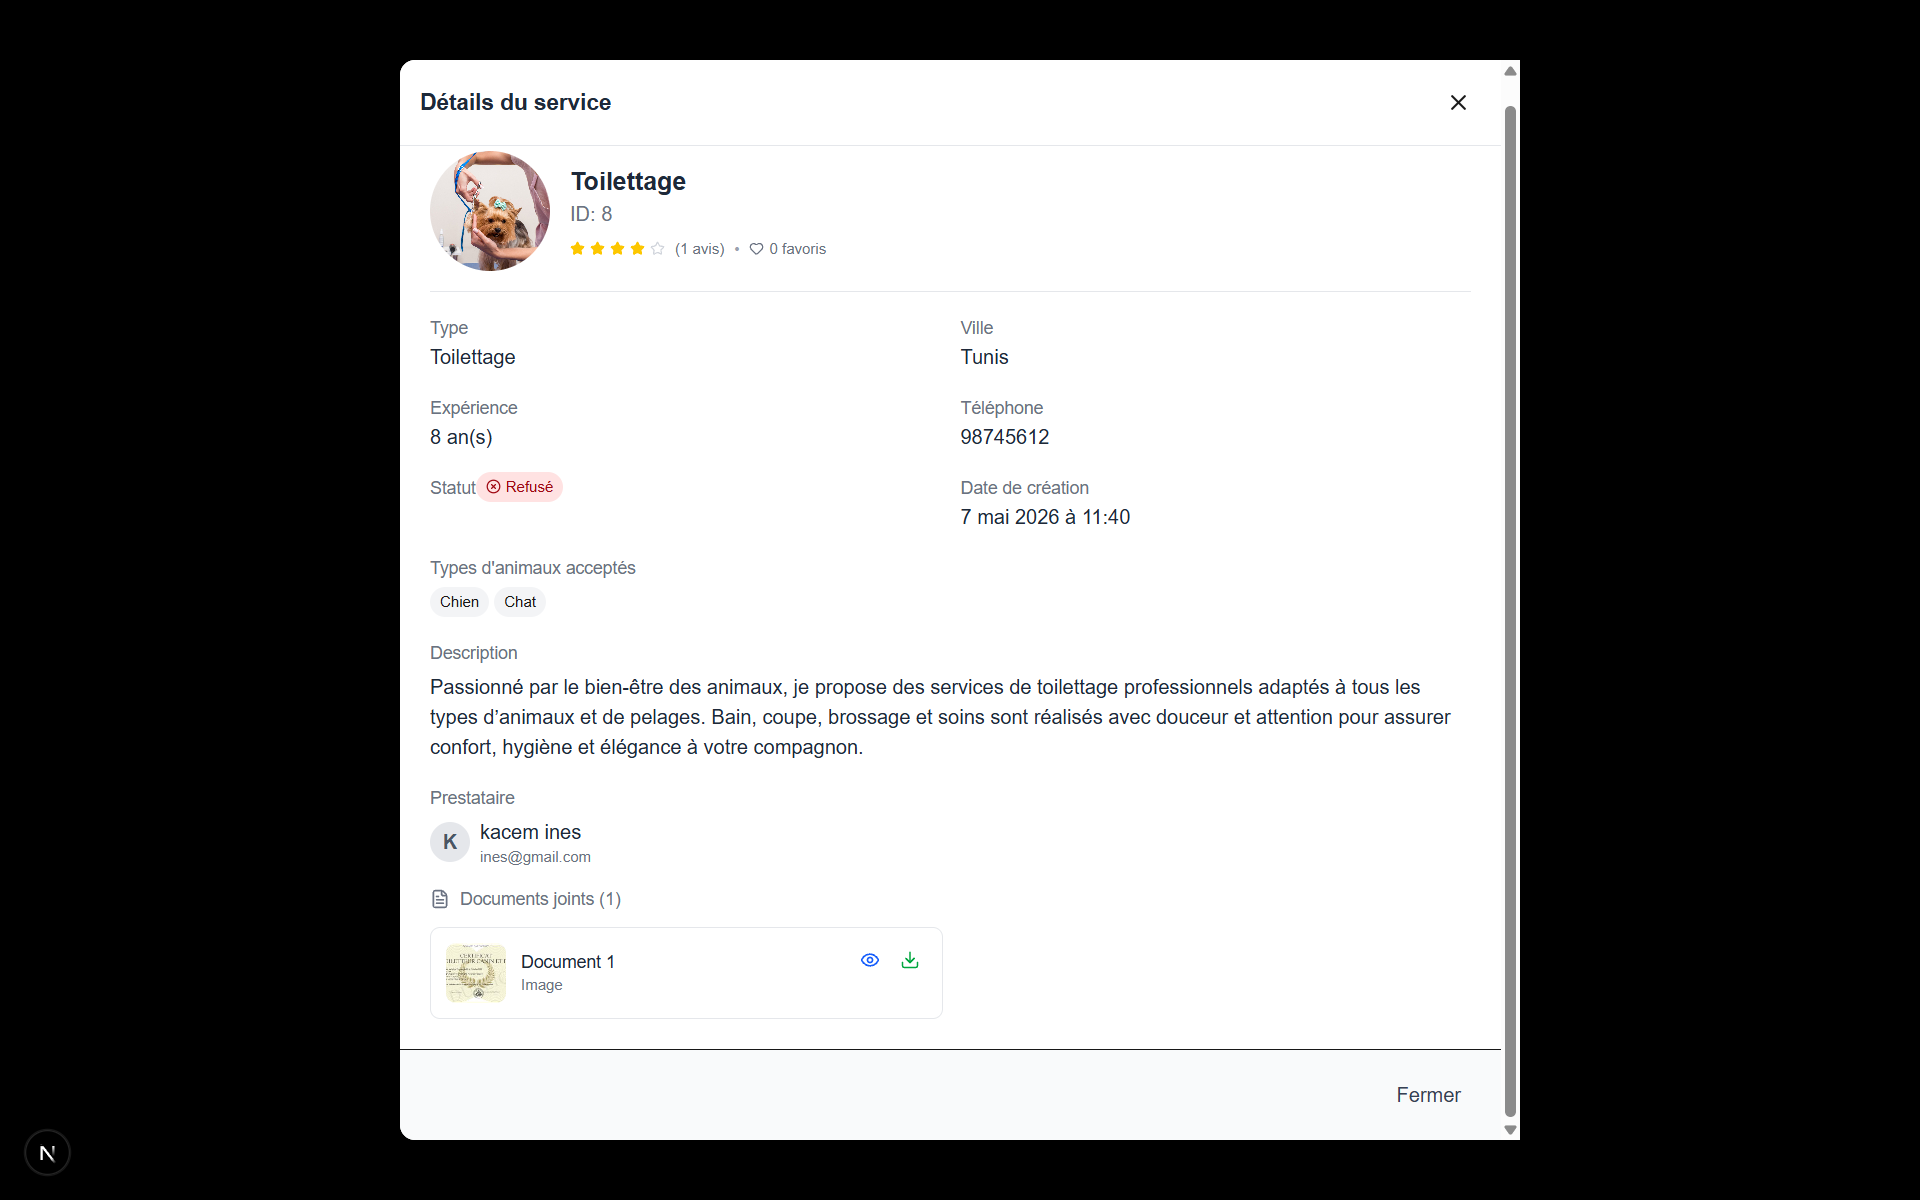
\includegraphics[width=0.8\textwidth]{images/dashboard anicare 2.png}
    \caption{Interface d’administration AniCare : vérification des services}
    \label{fig:anicare_verify}
\end{figure}

\subsubsection{Interfaces d’administration AniCare : statistiques AniCare}

Les figures \ref{fig:anicare_stats1} et \ref{fig:anicare_stats2} illustrent les statistiques du module AniCare, permettant à l’administrateur de suivre l’activité des services proposés sur la plateforme, le nombre de réservations effectuées ainsi que les interactions des utilisateurs avec les différents services disponibles : 
\begin{figure}[h!]
    \centering

    \begin{minipage}{0.48\textwidth}
        \centering
        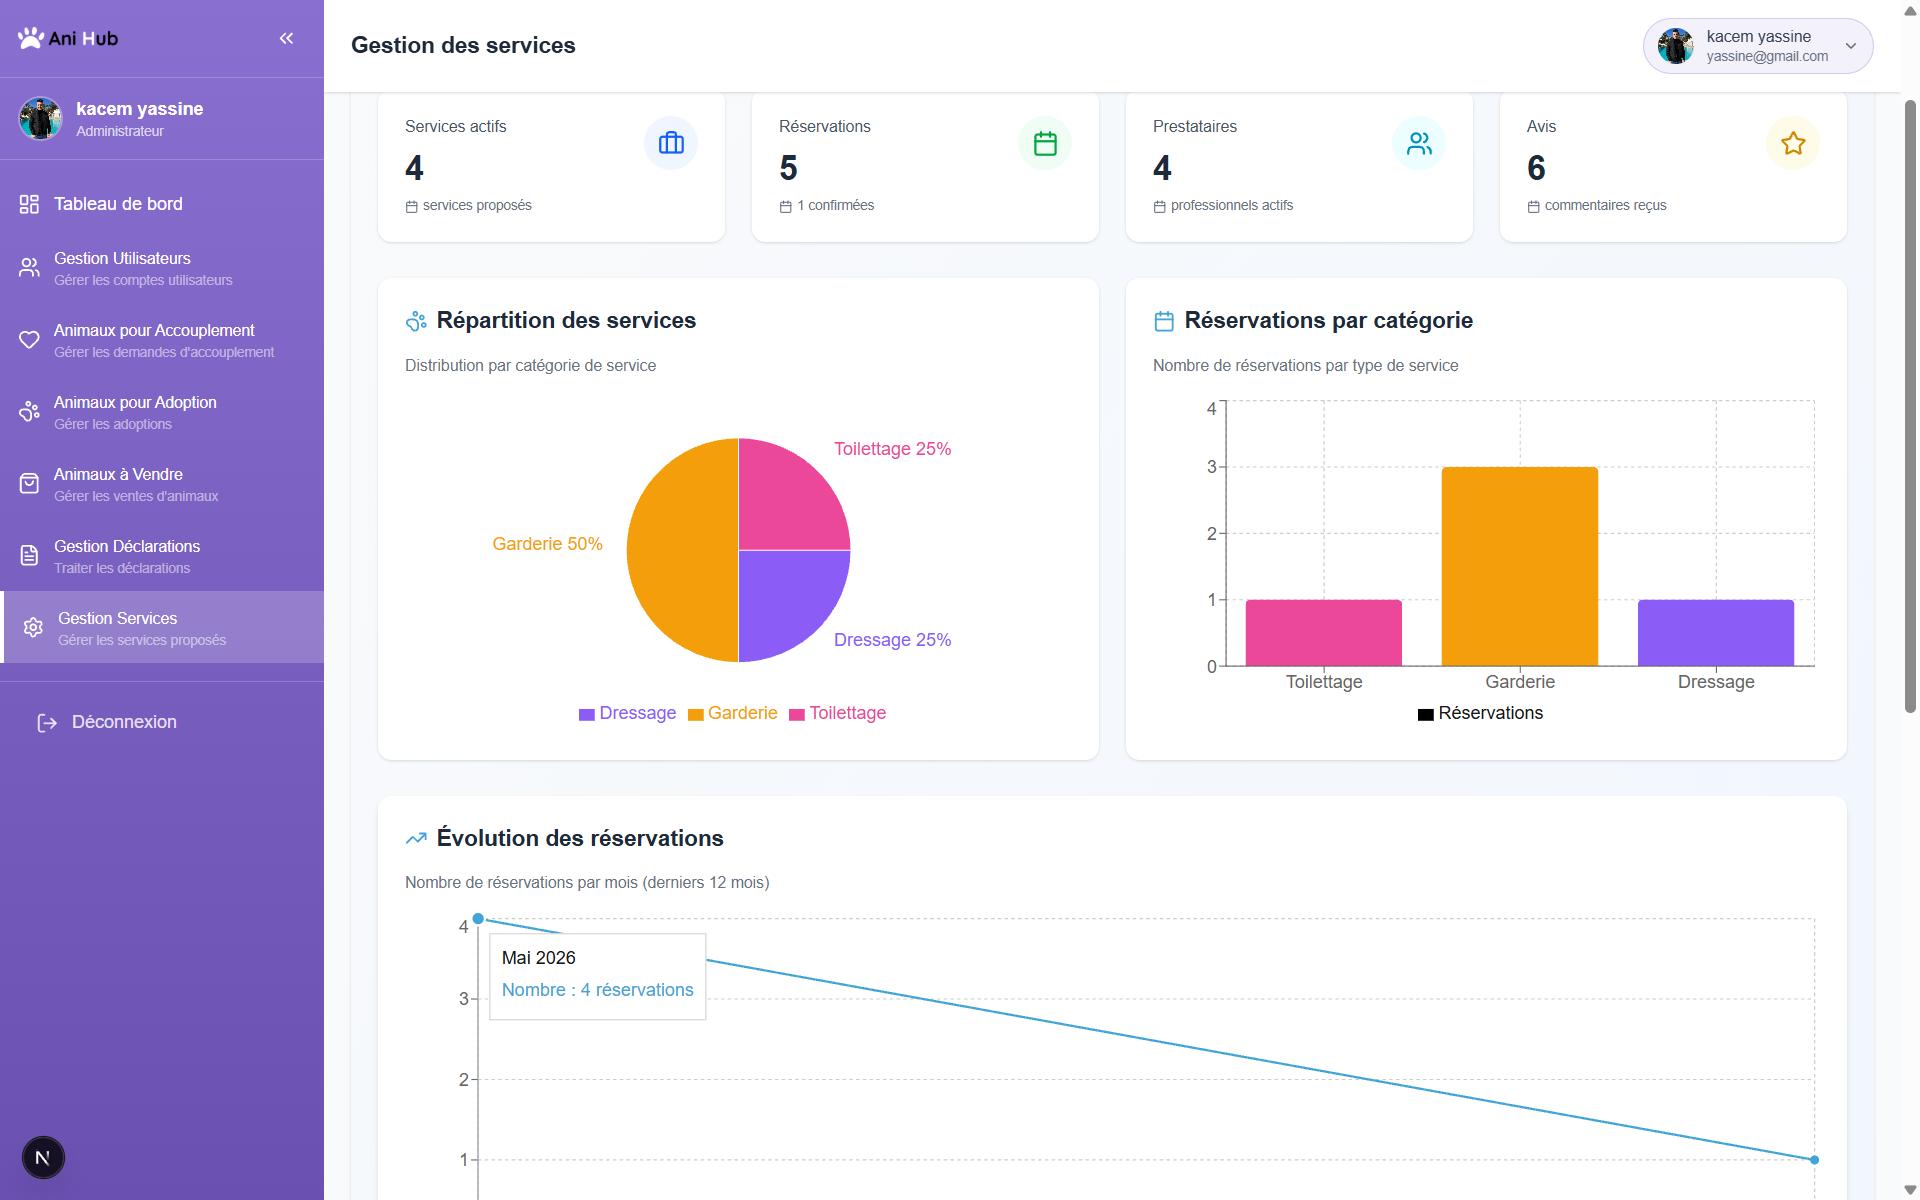
\includegraphics[width=\textwidth]{images/dashboard anicare 3.png}
        \caption{Interface de statistiques AniCare 1}
        \label{fig:anicare_stats1}
    \end{minipage}
    \hfill
    \begin{minipage}{0.48\textwidth}
        \centering
        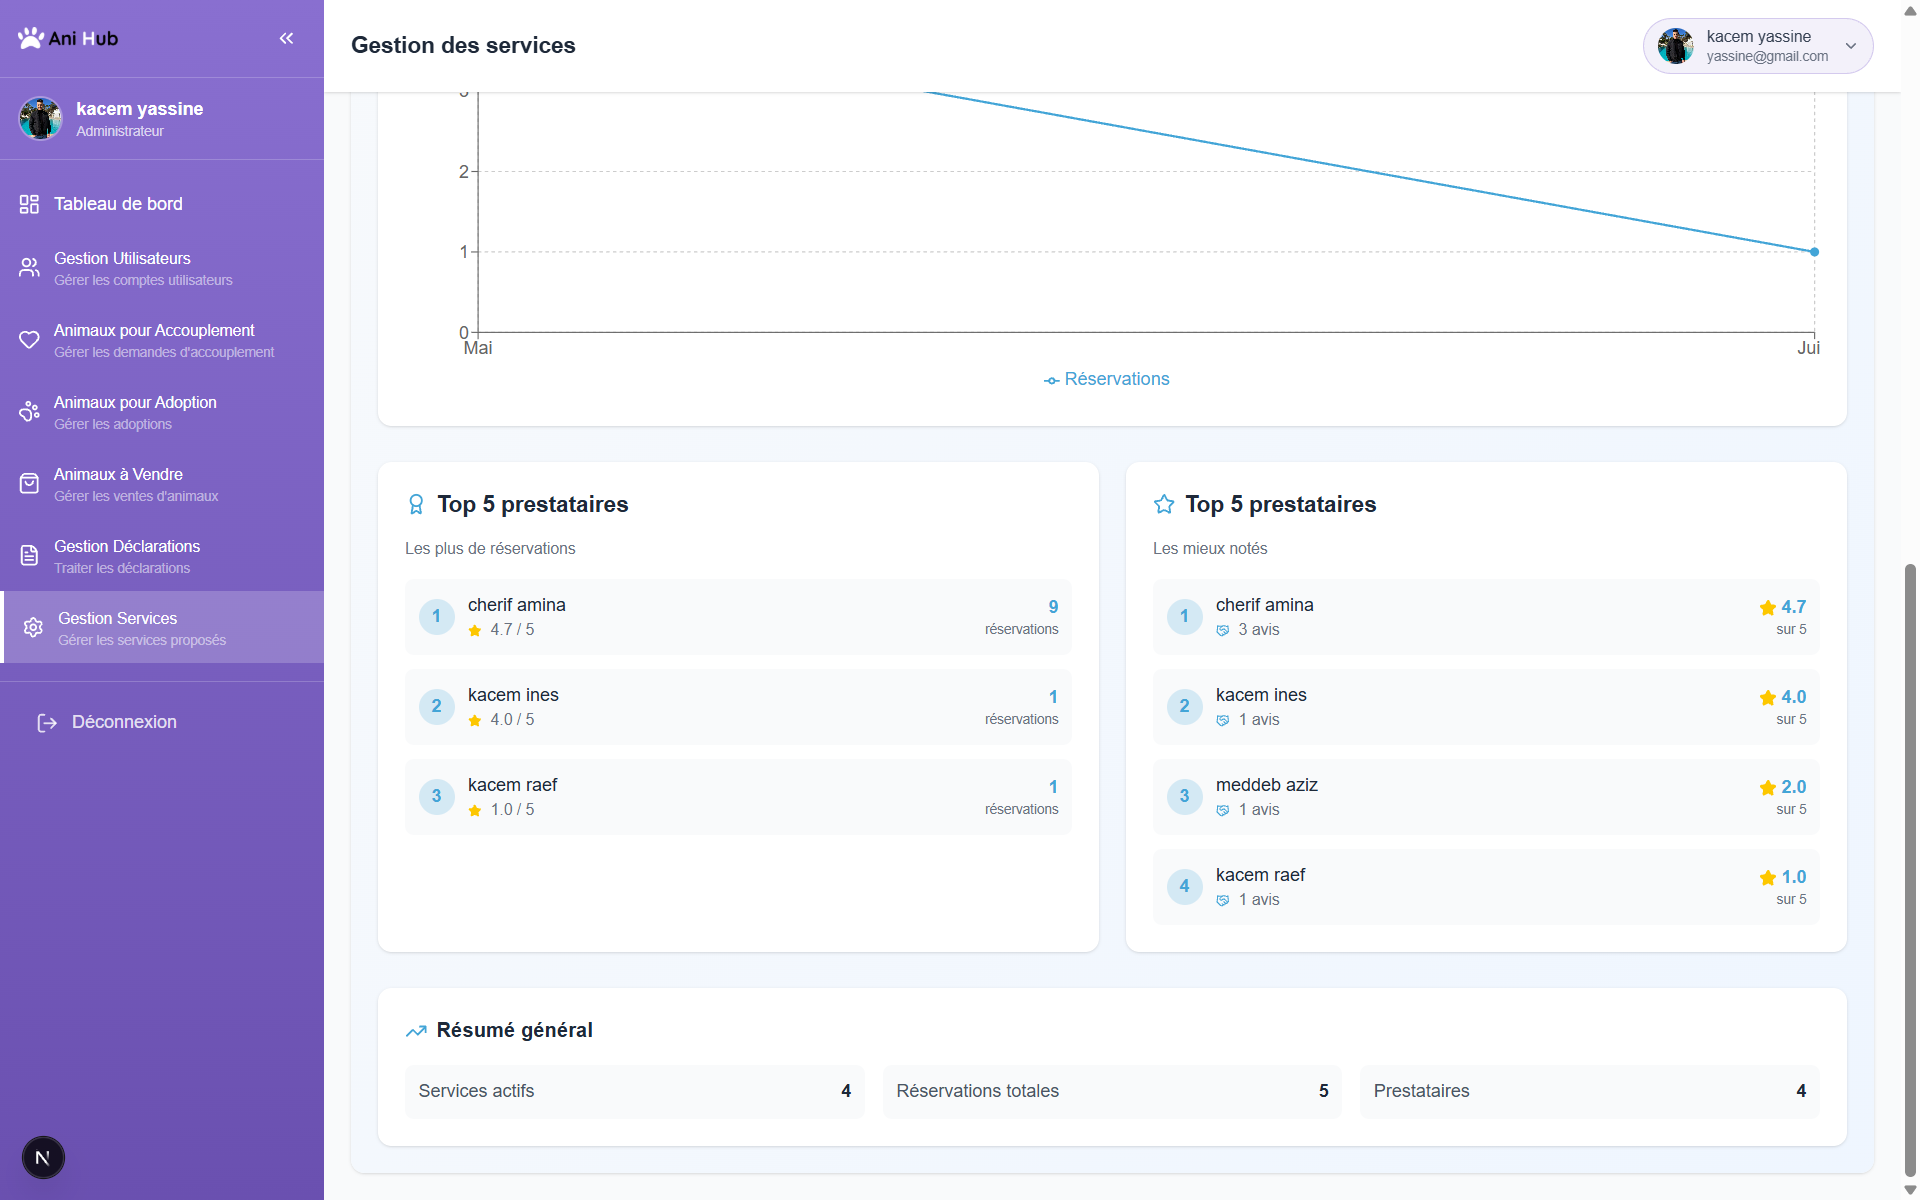
\includegraphics[width=\textwidth]{images/dashboard anicare 4.png}
        \caption{Interface de statistiques AniCare 2}
        \label{fig:anicare_stats2}
    \end{minipage}
\end{figure}






\section{Sprint 2 : Module AniMatch}
\begin{figure}[H]
    \centering
    
\includegraphics[width=3.8cm]{images/logo animatch 2.png}
    \caption{Logo du module AniMatch}
    \label{fig:logo-animatch}
\end{figure}
Ce sprint, d’une durée de \textbf{3 semaines}, est dédié au module AniMatch, qui permet la mise en relation entre propriétaires d’animaux pour l’adoption et l’accouplement. Il offre la possibilité de publier et consulter des annonces, d’échanger des invitations et de communiquer entre utilisateurs.  



\subsection{Sprint backlog} 
la table \ref{tab:sprint2-backlog} présente le Sprint Backlog du sprint 2 avec les user stories, les tâches associées et les efforts estimés : 
\begin{longtable}{|p{2cm}|p{5cm}|p{6cm}|p{2cm}|}
\caption{Sprint Backlog du sprint 2 }
\label{tab:sprint2-backlog} \\ 
\hline
\rowcolor{coloranimatch}
\textbf{ID} & \textbf{User Story} & \textbf{Tâches} & \textbf{Effort} \\
\hline
\endfirsthead

\hline
\rowcolor{coloranimatch}
\textbf{ID} & \textbf{User Story} & \textbf{Tâches} & \textbf{Effort} \\
\hline
\endhead

% ===================== US1=====================
\multirow{9}{2cm}{US1}
& \multirow{9}{5cm}{En tant qu’utilisateur, je
veux consulter la liste des animaux (adoption ou accouplement) afin de trouver un partenaire compatible}
& Conception UI (Figma) & 0.5 j \\
\cline{3-4}
& & API récupération des animaux & 1 j \\
\cline{3-4}
& & Filtrage et recherche & 1 j \\
\cline{3-4}
& & Pagination & 0.5 j \\
\cline{3-4}
& & Commentaires et notation des animaux & 1 j \\
\cline{3-4}
& & Intégration frontend/backend & 1 j \\
\hline

% ===================== US2 =====================
\multirow{10}{2cm}{US2}
& \multirow{10}{5cm}{En tant qu’utilisateur, je veux gérer mes annonces (publier, modifier et supprimer mes animaux) afin de maintenir mes informations à jour et trouver une correspondance}
& Conception UI (Figma) & 0.5 j \\
\cline{3-4}
& & APIs création , modification et suppression annonce & 1 j \\
\cline{3-4} 
& & Intégration avec microservice Auth (JWT, sécurité API) & 0.5 j \\
\cline{3-4}
& & Upload image (Cloudinary) & 1 j \\
\cline{3-4}
& & Intégration frontend/backend & 1 j \\ 
\cline{3-4} 
& & Tests & 0.5 j \\
\hline

% ===================== US3 =====================
\multirow{8}{2cm}{US3}
& \multirow{8}{5cm}{En tant qu’utilisateur, je veux gérer mes invitations envoyées afin de contrôler mes interactions}
& Conception UI "mon espace AniMatch"  (Figma) & 0.5 j \\
\cline{3-4}
& & API envoi, modification et annulation invitation & 1 j \\
\cline{3-4}
& & Gestion des statuts (en attente, acceptée, refusée) & 1 j \\ 
\cline{3-4} 
& & Intégration avec microservice Auth (JWT, sécurité API) & 0.5 j \\
\cline{3-4}
& & Intégration frontend/backend & 1 j \\
\hline

% ===================== US4 =====================
\multirow{5}{2cm}{US4}
& \multirow{5}{5cm}{En tant qu’utilisateur, je veux gérer les invitations reçues pour adoption ou accouplement afin de répondre aux demandes et gérer mes interactions}
& Conception UI (Figma) & 0.5 j \\
\cline{3-4}
& & API récupération des invitations reçues & 1 j \\
\cline{3-4}
& & APIs accepter , refuser invitation & 1 j \\
\cline{3-4}
& &  Gestion des statuts (acceptée, refusée)  & 0.5 j \\
\cline{3-4}
& & Intégration avec microservice Auth (JWT, sécurité API) & 0.5 j \\ 
\cline{3-4} 
& & Intégration frontend/backend & 1 j \\ 
\cline{3-4}  
\cline{3-4}
& & Tests & 0.5 j \\
\hline

% ===================== US5 =====================
\multirow{6}{2cm}{US5}
& \multirow{6}{5cm}{En tant qu’utilisateur, je veux gérer mes notifications afin d’être informé des interactions sur mes annonces et activités sur Animatch}
& Analyse besoins notifications & 0.5 j \\
\cline{3-4}
& & Développement microservice Notifications & 1 j \\
\cline{3-4}
& & Intégration RabbitMQ avec Microservice AniMatch & 1 j \\
\cline{3-4}
& & Intégration RabbitMQ avec Microservice Notifications & 1 j \\
\cline{3-4}
& & Création événements (invitations, intérêts, acceptation, etc.) & 0.5 j \\
\cline{3-4}
& & Interface notifications frontend & 0.5 j \\
\cline{3-4}
& & Marquer comme lu / non lu & 0.5 j \\ 
\cline{3-4}
& & Tests & 0.5 j \\
\hline

% ===================== US8 =====================
\multirow{4}{2cm}{US6}
& \multirow{4}{5cm}{En tant qu’utilisateur, je veux discuter avec un autre propriétaire}
& Analyse & 0.5 j \\
\cline{3-4}
& & Intégration bouton WhatsApp & 0.5 j \\
\cline{3-4}
& & Génération lien wa.me & 0.5 j \\
\cline{3-4}
& & Tests & 0.5 j \\
\hline

\end{longtable}
\newpage
\subsection{Diagramme des cas d’utilisation du sprint 2}

Dans cette section, nous présentons le diagramme des cas d’utilisation du deuxième sprint, dédié au module \textbf{AniMatch}. 

 Ce diagramme illustre les principales interactions entre l’utilisateur et le système, notamment la gestion des annonces, des invitations et des communications.

La figure \ref{fig:usecase-sprint2} représente le diagramme des cas d’utilisation correspondant.

\begin{figure}[H]
    \centering
  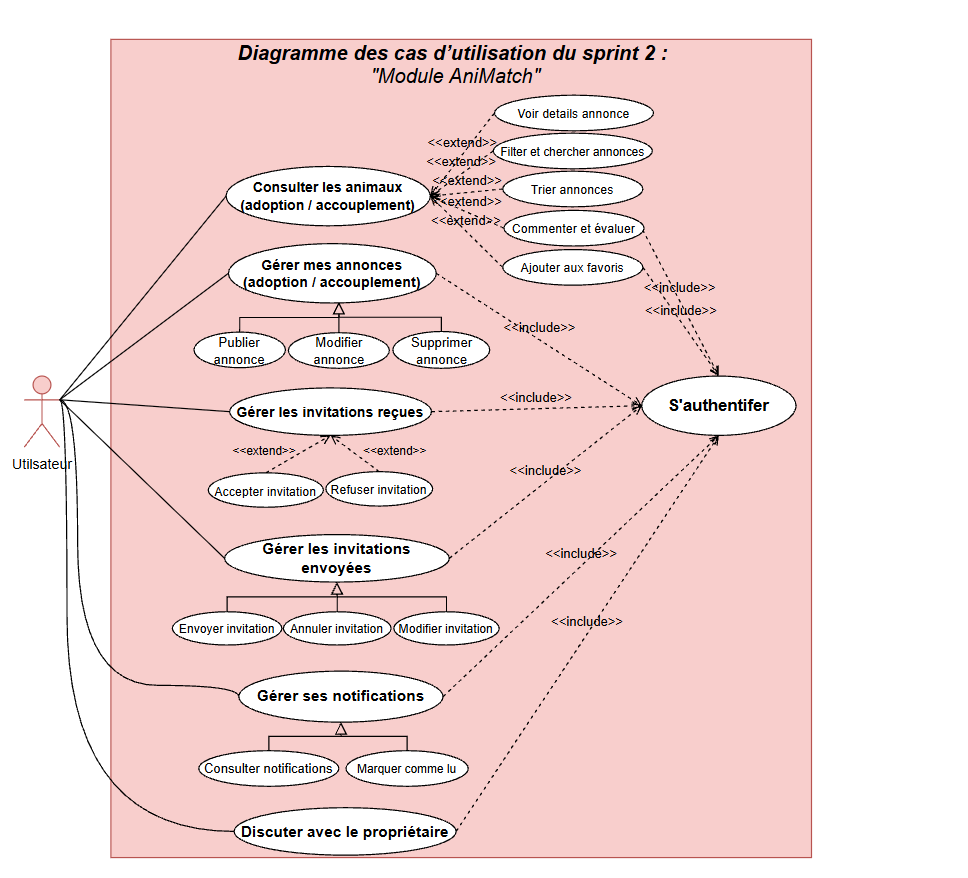
\includegraphics[width=1.05\linewidth, height=19.5cm, keepaspectratio]{images/usecase animatch.png}
    \caption{Diagramme des cas d’utilisation du sprint 2}
    \label{fig:usecase-sprint2}
\end{figure}


\newpage
\subsection{Descriptions textuelles des cas d’utilisation du sprint 2}   
Cette section présente les cas d’utilisation du sprint 2 du module AniMatch : 
\subsubsection{ Description textuelle du cas d’utilisation «Consulter les animaux pour adoption et accouplement» } 
La table \ref{tab:consulter_annonces} présente le cas d’utilisation « Consulter les animaux pour adoption et accouplement » : 
\begin{longtable}{|c|p{11cm}|}
\caption{Description textuelle du cas d’utilisation "Consulter les animaux pour adoption et accouplement"}
\label{tab:consulter_annonces} \\
\hline
\cellcolor{coloranimatch} \textbf{Nom du cas d'utilisation } & Consulter les annonces d’accouplement et d’adoption \\
\hline
\cellcolor{coloranimatch} \textbf{Acteurs} & Utilisateur \\
\hline
\cellcolor{coloranimatch} \textbf{Description } & Tout utilisateur du site peut consulter les annonces du module AniMatch, notamment celles d’adoption et d’accouplement. \\
\hline
\cellcolor{coloranimatch} \textbf{Pré-condition } & Accès libre à la page d’accueil sans authentification. \\
\hline
\cellcolor{coloranimatch} \textbf{Post-condition } & L’utilisateur a consulté les annonces et peut interagir . \\
\hline

\cellcolor{coloranimatch} \textbf{Scénario nominal } & 
\begin{enumerate}
\item L’utilisateur accède à la page d’accueil d’AniHub.
\item L’utilisateur choisit le module AniMatch.
\item Le système redirige l’utilisateur vers AniMatch.
\item L’utilisateur choisit "adoption" ou "accouplement".
\item Le système redirige vers la section choisie.
\item L’utilisateur peut filtrer les annonces selon des critères.
\item Le système affiche la liste des annonces filtrés.
\item L’utilisateur clique sur une annonce .
\item Le système affiche les détails de l’annonce.
\item L’utilisateur authentifié ajoute une annonce à sa (wishlist).
\item Le système ajoute l’annonce à sa wishlist .
\item L’utilisateur authentifié peut saisir un commentaire , attribuer une note clique sur « Publier ».
\item Le système vérifie , enregistre le commentaire et la note et met à jour la liste des avis affichés.
\end{enumerate} \\

\hline
\cellcolor{coloranimatch} \textbf{Scénario alternatif :} &
Message d’erreur affiché si l’utilisateur n’est pas authentifié lors de l’ajout aux favoris ou de la publication d’un commentaire. \\
\hline

\end{longtable}


\newpage 
\subsubsection{Description textuelle du cas d’utilisation «Gérer mes annonces dans AniMatch»} 
La table \ref{tab:gerer_annonces_global} présente le cas d’utilisation « Gérer mes  annonces d’accouplement et d’adoption » : 
\begin{longtable}{|c|p{11cm}|}
\caption{Description textuelle du cas d'utilisation "Gérer les annonces d’accouplement et d’adoption"}
\label{tab:gerer_annonces_global} \\
\hline
\cellcolor{coloranimatch}\textbf{Nom du cas d'utilisation } & Gérer mes annonces d’accouplement et d’adoption \\
\hline
\cellcolor{coloranimatch}\textbf{Acteurs} & Utilisateur \\
\hline
\cellcolor{coloranimatch}\textbf{Description } & L’utilisateur peut publier, modifier ou supprimer une annonce \\
\hline
\cellcolor{coloranimatch}\textbf{Pré-condition } & L’utilisateur doit être authentifié  \\
\hline
\cellcolor{coloranimatch}\textbf{Post-condition } & L’annonce est ajoutée, modifiée ou supprimée avec succès. \\
\hline

\cellcolor{coloranimatch}\textbf{Scénario nominal } &
\begin{enumerate}
\item L’utilisateur accède au module AniMatch.
\item Le système redirige l’utilisateur vers "AniMatch".

\item \textbf{Cas publication :}
\begin{itemize}
\item L’utilisateur choisit "adoption" ou "accouplement".
\item Le système redirige vers la section choisie.
\item L’utilisateur clique sur « Annoncer mon animal ».
\item Le système affiche le formulaire d’ajout.
\item L’utilisateur remplit les informations et valide.
\item Le système vérifie et enregistre l’annonce.
\end{itemize}

\item L’utilisateur accède à « Mon espace AniMatch ».
\item Le système affiche ses annonces.

\item \textbf{Cas modification :}
\begin{itemize}
\item L’utilisateur sélectionne une annonce.
\item L’utilisateur clique sur « Modifier ».
\item Le système affiche le formulaire pré-rempli.
\item L’utilisateur modifie et valide.
\item Le système enregistre les modifications.
\end{itemize}

\item \textbf{Cas suppression :}
\begin{itemize}
\item L’utilisateur sélectionne une annonce.
\item L’utilisateur clique sur « Supprimer ».
\item Le système demande une confirmation.
\item L’utilisateur confirme.
\item Le système supprime l’annonce.
\end{itemize}

\item Le système affiche un message de succès.
\end{enumerate} \\

\hline
\cellcolor{coloranimatch}\textbf{Scénario alternatif :} &
\begin{itemize}
\item Erreur de publication ou modification : message d’erreur affiché.
\item Annulation de la suppression : l’annonce est conservée.
\end{itemize} \\
\hline

\end{longtable}
\newpage
\subsubsection{ Description textuelle du cas d’utilisation «Gérer les invitations reçues» }   
La table \ref{tab:gerer_invitations} illustre la description textuelle du cas d’utilisation « Gérer les invitations reçues d’accouplement et d’adoption », qui détaille les différentes interactions entre l’utilisateur et le système : 
\begin{longtable}{|c|p{11cm}|}
\caption{Description textuelle du cas d'utilisation "Gérer les invitations reçues (adoption / accouplement)"}
\label{tab:gerer_invitations} \\
\hline
\cellcolor{coloranimatch}\textbf{Nom du cas d'utilisation } & Gérer les invitations reçues (adoption / accouplement) \\
\hline
\cellcolor{coloranimatch}\textbf{Acteurs} & Utilisateur \\
\hline
\cellcolor{coloranimatch}\textbf{Description } & L’utilisateur consulte et gère les invitations reçues pour adoption ou accouplement en décidant de les accepter ou de les refuser. \\
\hline
\cellcolor{coloranimatch}\textbf{Pré-condition } & L’utilisateur est authentifié et dispose d’au moins une invitation reçue. \\
\hline
\cellcolor{coloranimatch}\textbf{Post-condition } & Le statut de l’invitation est mis à jour et la réponse est enregistrée par le système. \\
\hline
\cellcolor{coloranimatch}\textbf{Scénario nominal } &
\begin{enumerate}
\item L’utilisateur se connecte à son compte et accède au module AniMatch.
\item Il sélectionne « Mon espace AniMatch » depuis la barre de navigation.
\item Le système affiche la liste des invitations reçues.
\item L’utilisateur consulte une invitation et accède à ses détails.  
Selon le type :
\begin{itemize}
\item Accouplement : affichage des informations de l’animal proposé.
\item Adoption : affichage des informations de l’utilisateur et de sa demande.
\end{itemize}
\item L’utilisateur choisit une invitation.
\item Il clique sur « Accepter » ou « Refuser ».
\item Le système enregistre la réponse et met à jour le statut.
\item Le système affiche un message de confirmation.
\end{enumerate} \\
\hline
\cellcolor{coloranimatch}\textbf{Scénario alternatif :} &
\begin{itemize}
\item Aucune invitation reçue : le système affiche un message indiquant que la liste est vide.
\item Erreur lors du traitement : le système affiche un message d’erreur sans modifier l’état.
\end{itemize} \\
\hline
\end{longtable}  

\newpage
\subsection{Diagramme de classes du sprint 2}
La figure \ref{fig:class_diagram_sprint2} représente le diagramme de classes du sprint 2 dédié au module AniMatch, illustrant les principales entités du système ainsi que leurs relations pour assurer le bon fonctionnement du module : 
\begin{figure}[H]
    \centering
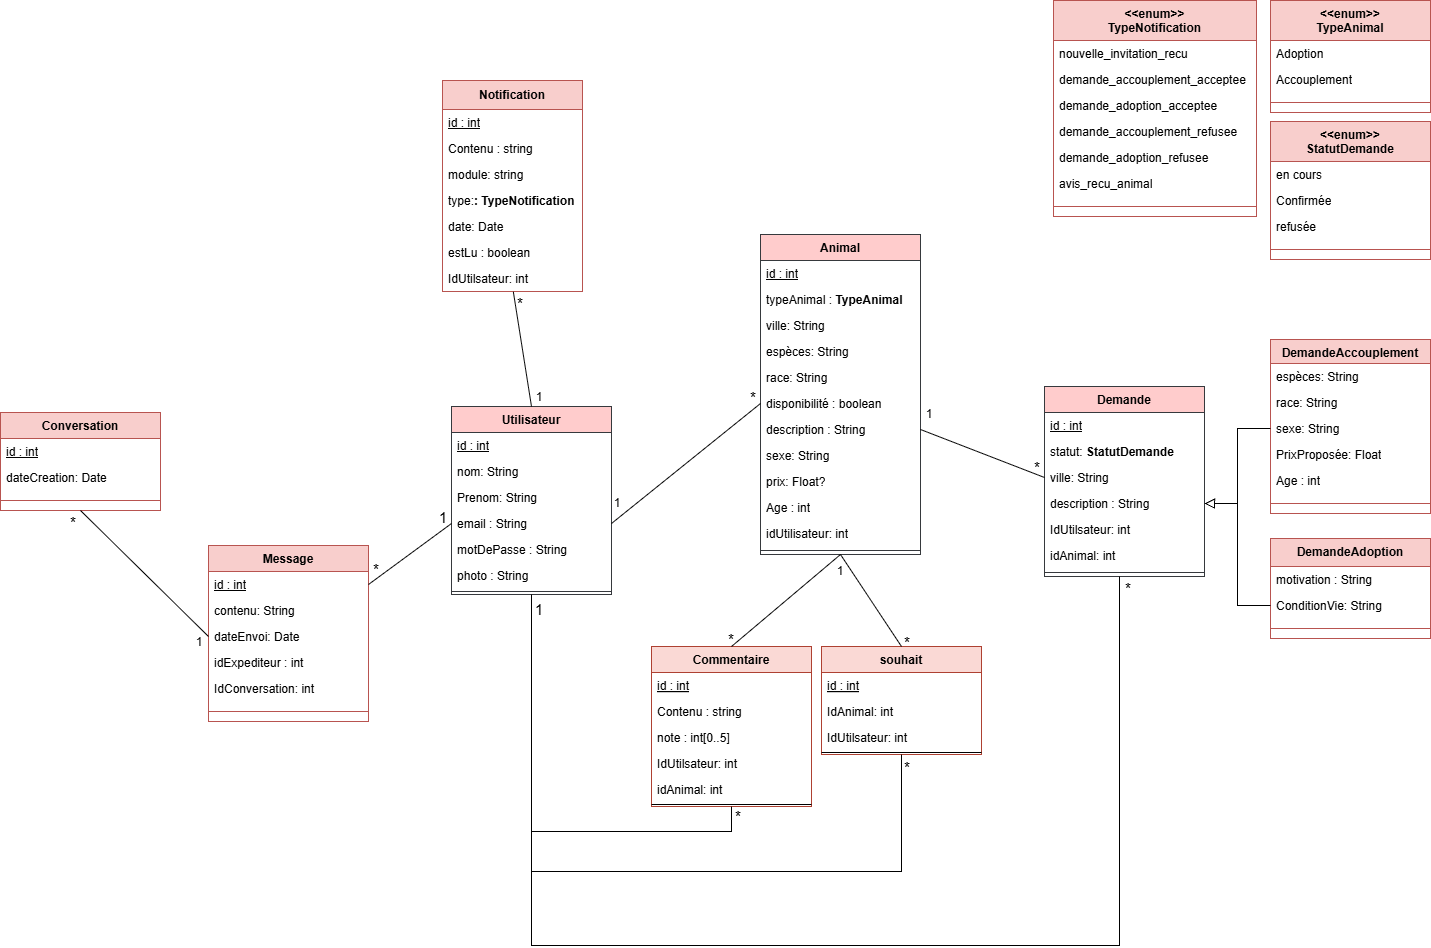
\includegraphics[width=1\textwidth]{images/diagramme classes animatch.png}
    \caption{Diagramme de classes de la sprint 2}
    \label{fig:class_diagram_sprint2}
\end{figure}  


\subsection{Diagrammes de séquences du sprint 2} 
Cette section présente les diagrammes de séquences du deuxieme sprint, illustrant les interactions entre les différents composants du système. 
\subsubsection{Diagramme de séquence : Gérer mes animaux pour accouplement et pour adoption}

Cette figure \ref{fig:gerer_animaux_animatch_seq} illustre les différentes interactions permettant à l’utilisateur de gérer ses animaux destinés à l’accouplement ou à l’adoption.

\newpage
\begin{figure}[H]
    \centering
    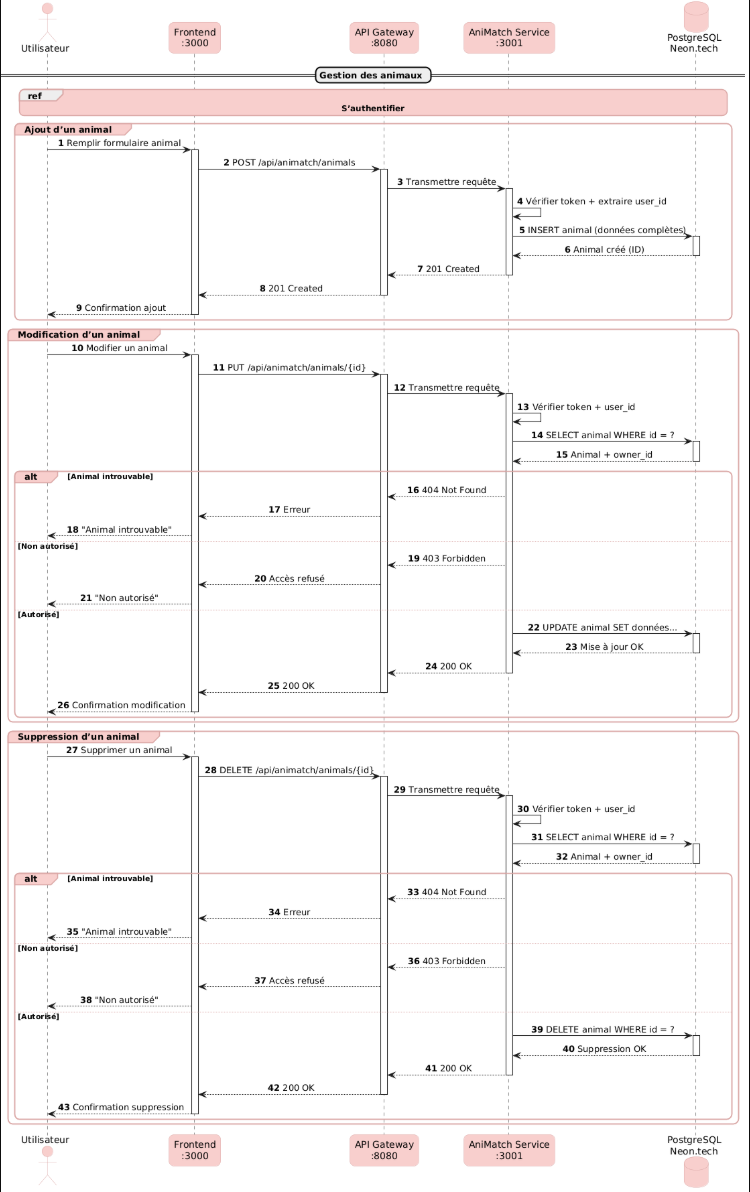
\includegraphics[width=0.75\textwidth]{images/gerer mes animaux animatch sq.png}
    \caption{Diagramme de séquence : gérer mes animaux pour accouplement et pour adoption}
    \label{fig:gerer_animaux_animatch_seq}
\end{figure}
\newpage 
\subsubsection{Diagramme de séquence : gérer mes invitations reçues}

Cette figure \ref{fig:gerer_invitations_recues_seq} illustre les interactions entre les composants du système lors de la gestion des invitations reçues. L’utilisateur peut consulter une invitation puis l’accepter ou la refuser. Le système met ensuite à jour son statut et envoie une notification aux utilisateurs concernés.

\begin{figure}[H]
    \centering
    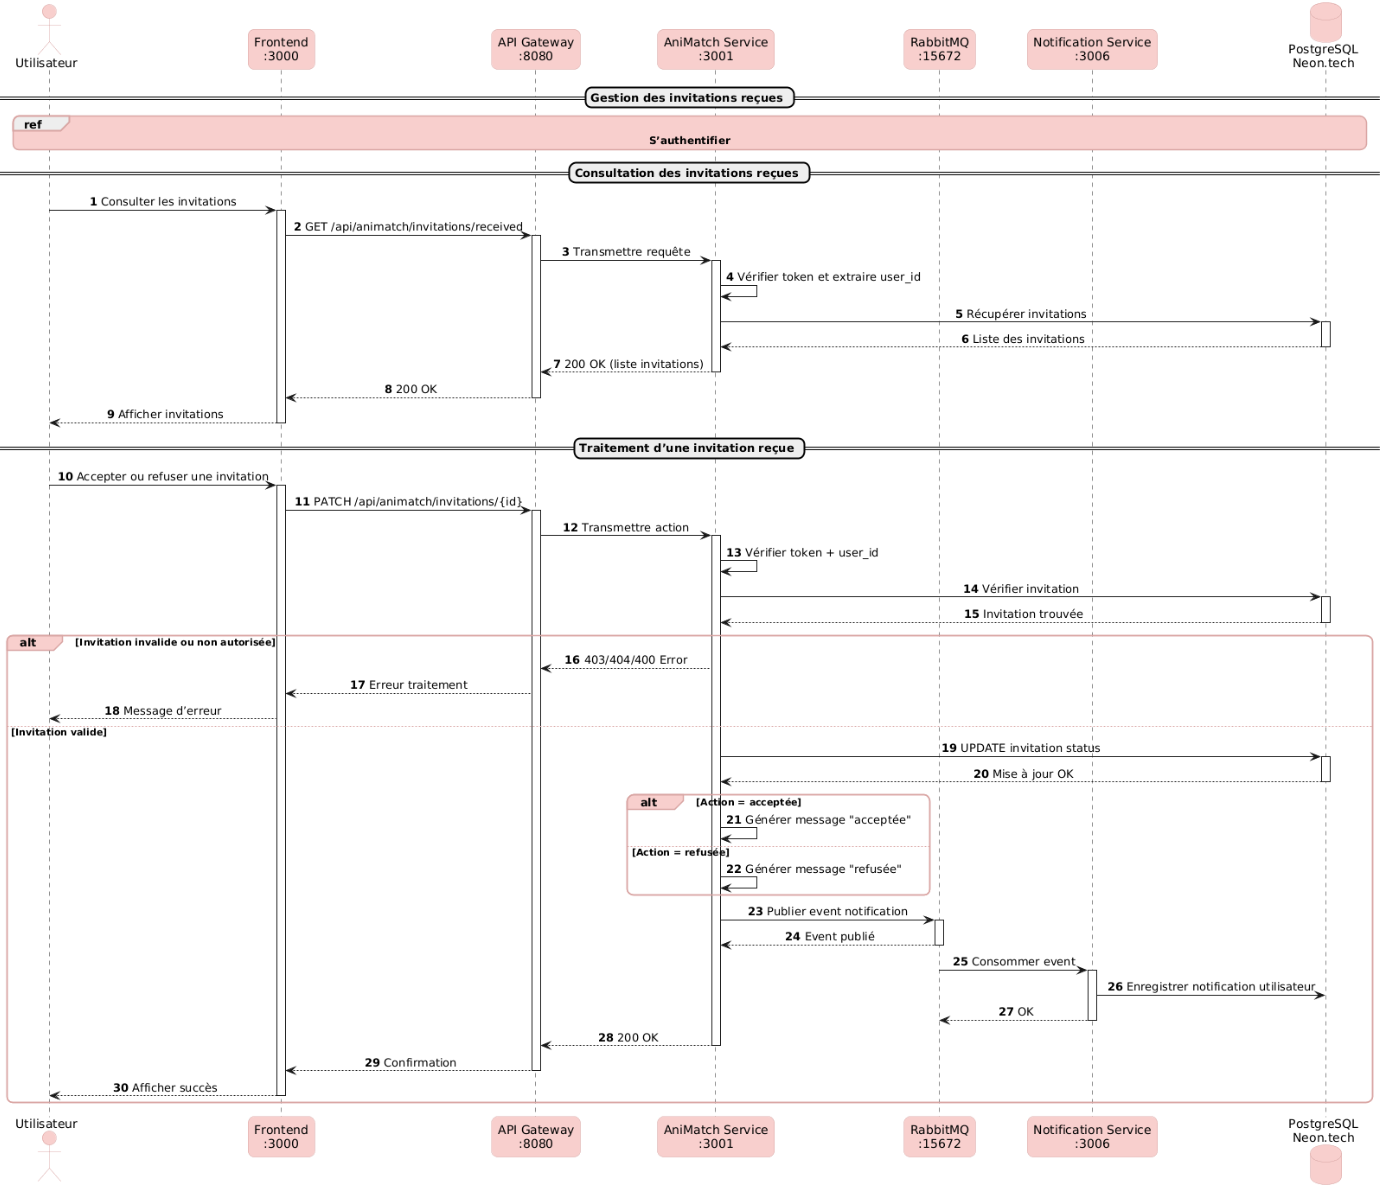
\includegraphics[width=1\textwidth]{images/gerer inv recus sq.png}
    \caption{Diagramme de séquence : gérer mes invitations reçues}
    \label{fig:gerer_invitations_recues_seq}
\end{figure}
\newpage 
\subsubsection{Diagramme de séquence : gérer mes invitations envoyées}

Cette figure \ref{fig:gerer_invitations_envoyees_seq} illustre les interactions entre les composants du système lors de la gestion des invitations envoyées. L’utilisateur peut consulter les invitations qu’il a envoyées et suivre leur état. Le système assure également la mise à jour des informations et l’envoi des notifications aux utilisateurs concernés.

\begin{figure}[H]
    \centering
    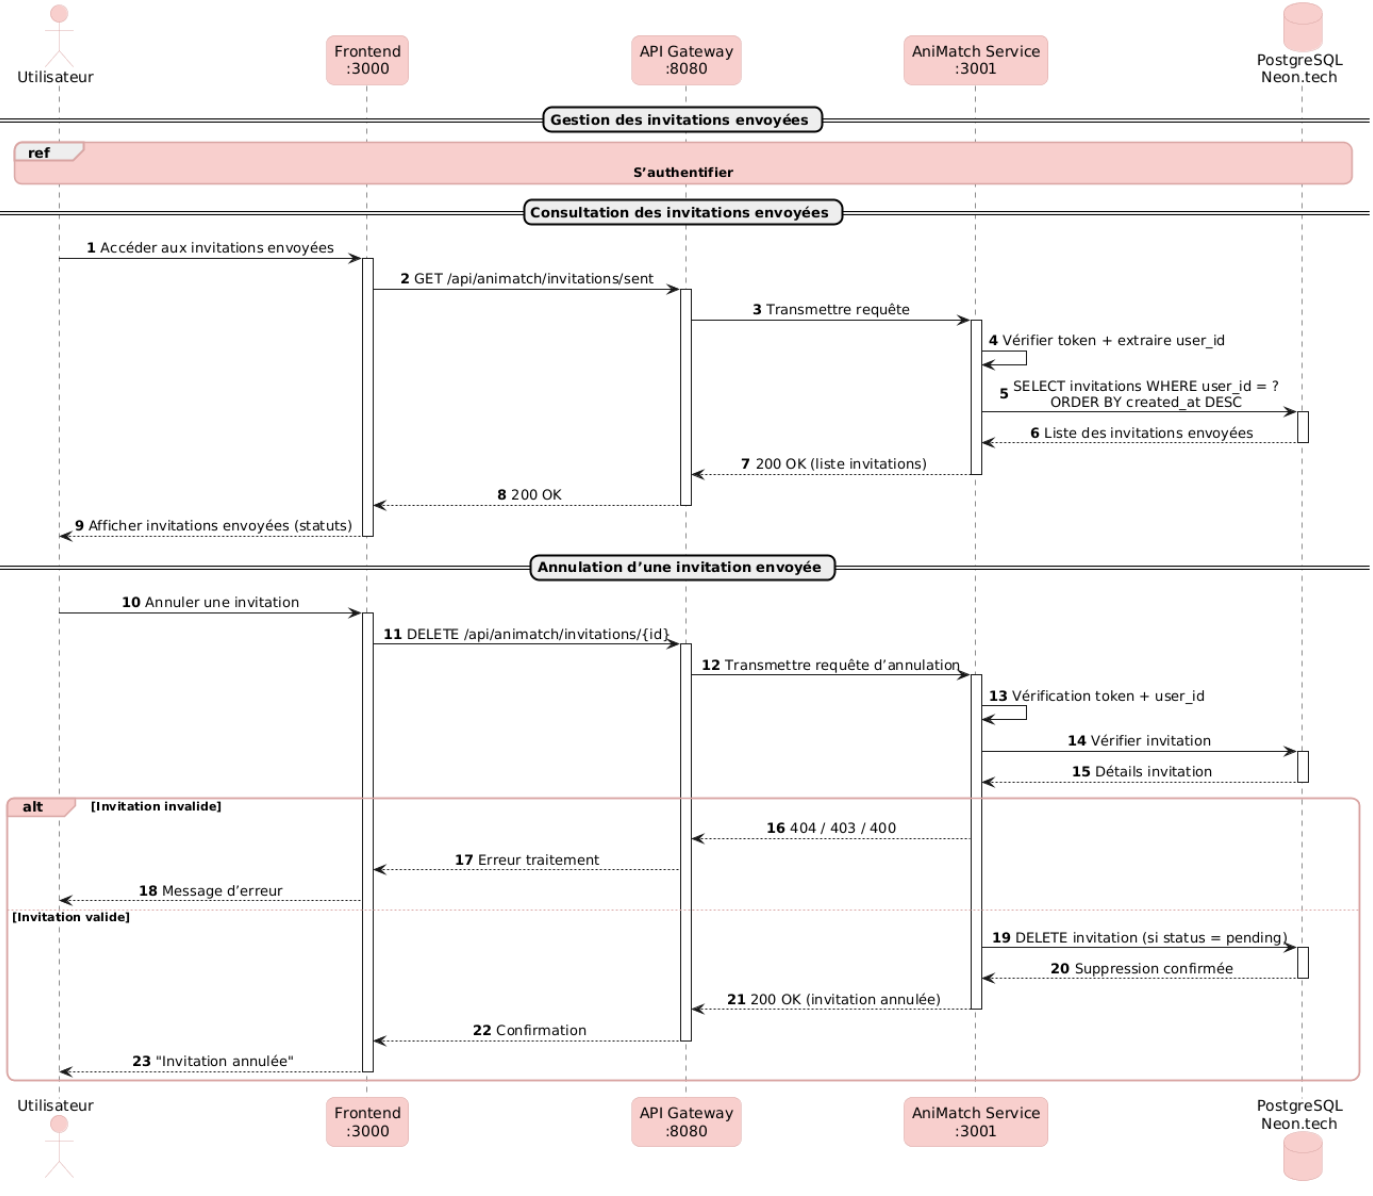
\includegraphics[width=1\textwidth]{images/gerer inv envoyes sq.png}
    \caption{Diagramme de séquence : gérer mes invitations envoyées}
    \label{fig:gerer_invitations_envoyees_seq}
\end{figure}

\newpage
\subsection{Réalisation du sprint 2} 

Dans cette partie, nous allons présenter les différentes interfaces graphiques de l’application développée, en lien avec les cas d’utilisation de cette sprint . 
\subsubsection{Interfaces d’accueil et menu principal de l’application AniHub}

Les figures \ref{fig:acceuil_anihub} et \ref{fig:menu_anihub} illustrent respectivement l’interface d’accueil de l’application AniHub et le menu principal permettant d’accéder aux différents modules de la plateforme.

\begin{figure}[h!]
    \centering
    
    \begin{minipage}{0.48\textwidth}
        \centering
        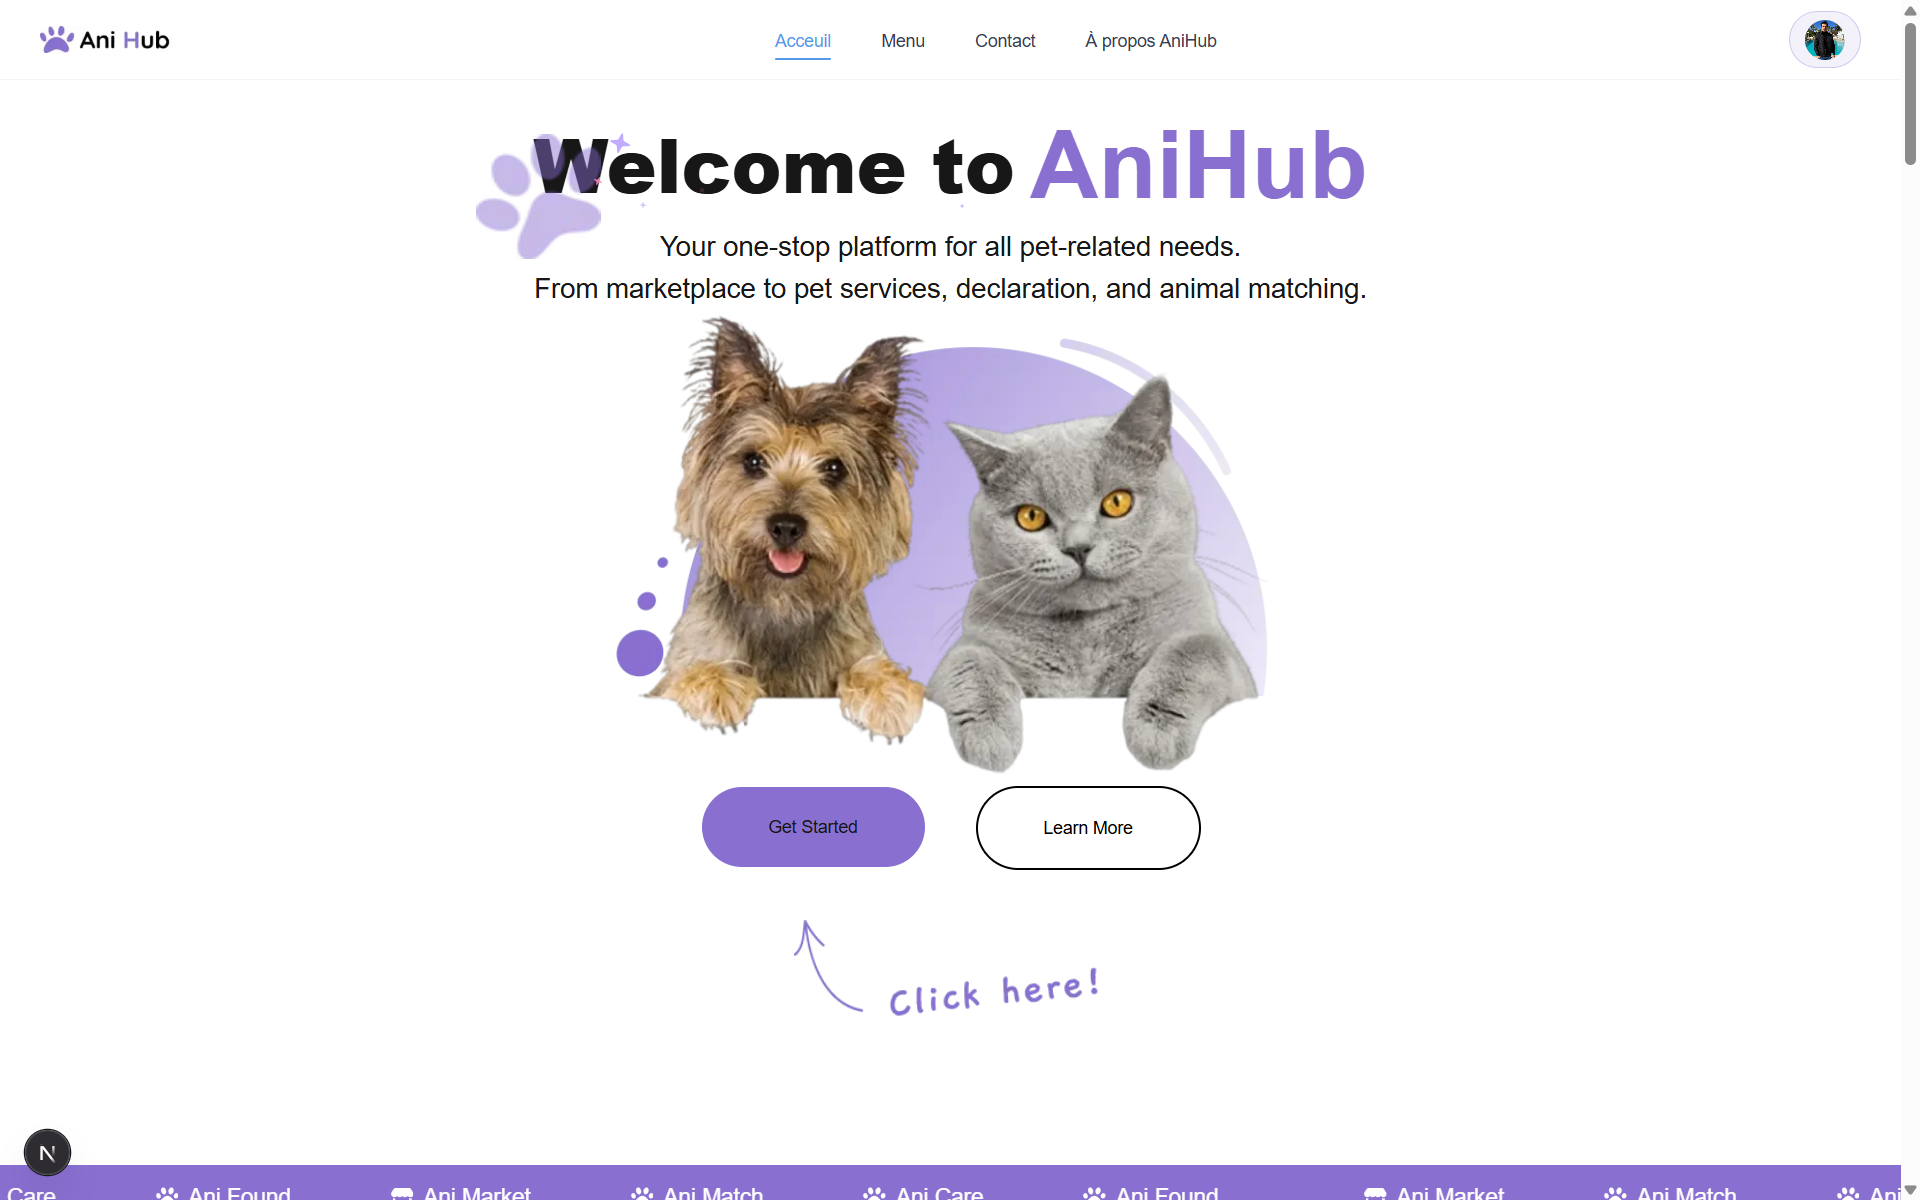
\includegraphics[width=\textwidth]{images/acceuil.png}
        \caption{Interface d’accueil AniHub}
        \label{fig:acceuil_anihub}
    \end{minipage}
    \hfill
    \begin{minipage}{0.48\textwidth}
        \centering
        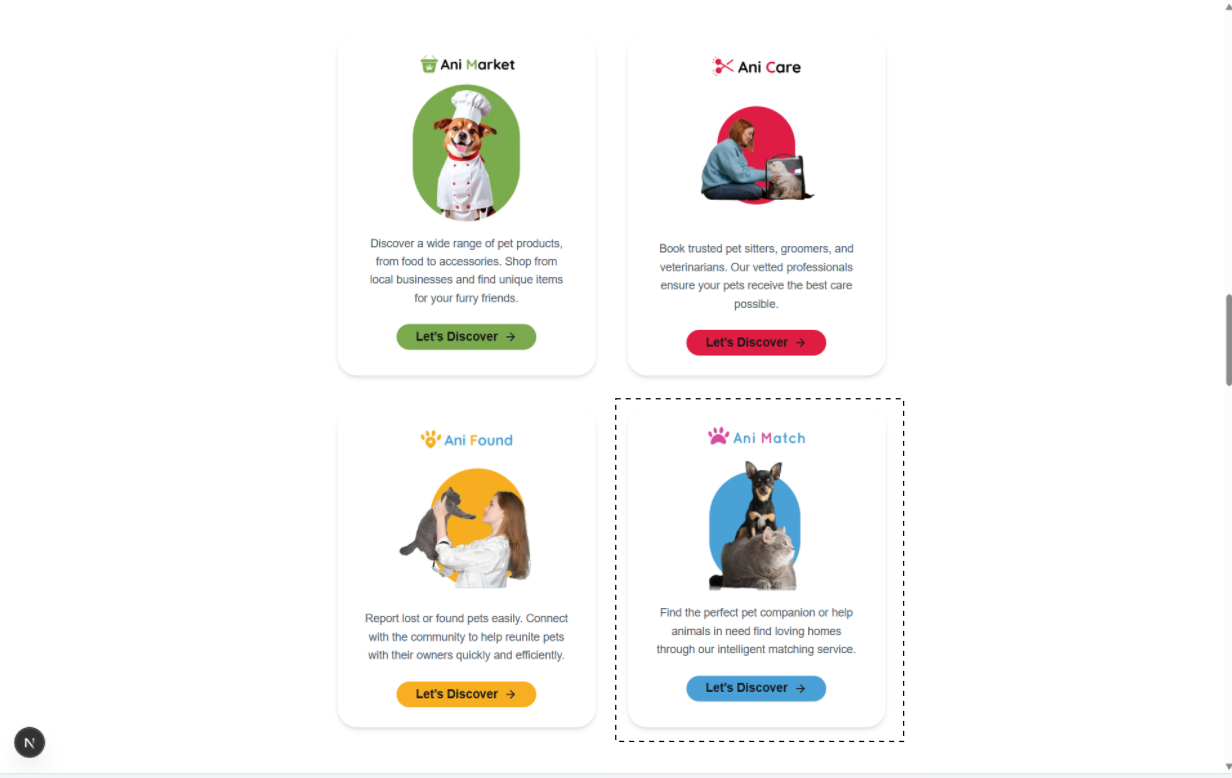
\includegraphics[width=\textwidth]{images/menu.png}
        \caption{Menu principal AniHub}
        \label{fig:menu_anihub}
    \end{minipage}

\end{figure} 

\subsubsection{Interface d’accueil AniMatch}

La figure \ref{fig:acceuil_animatch} illustre l’interface d’accueil du module AniMatch :

\begin{figure}[h!]
    \centering
    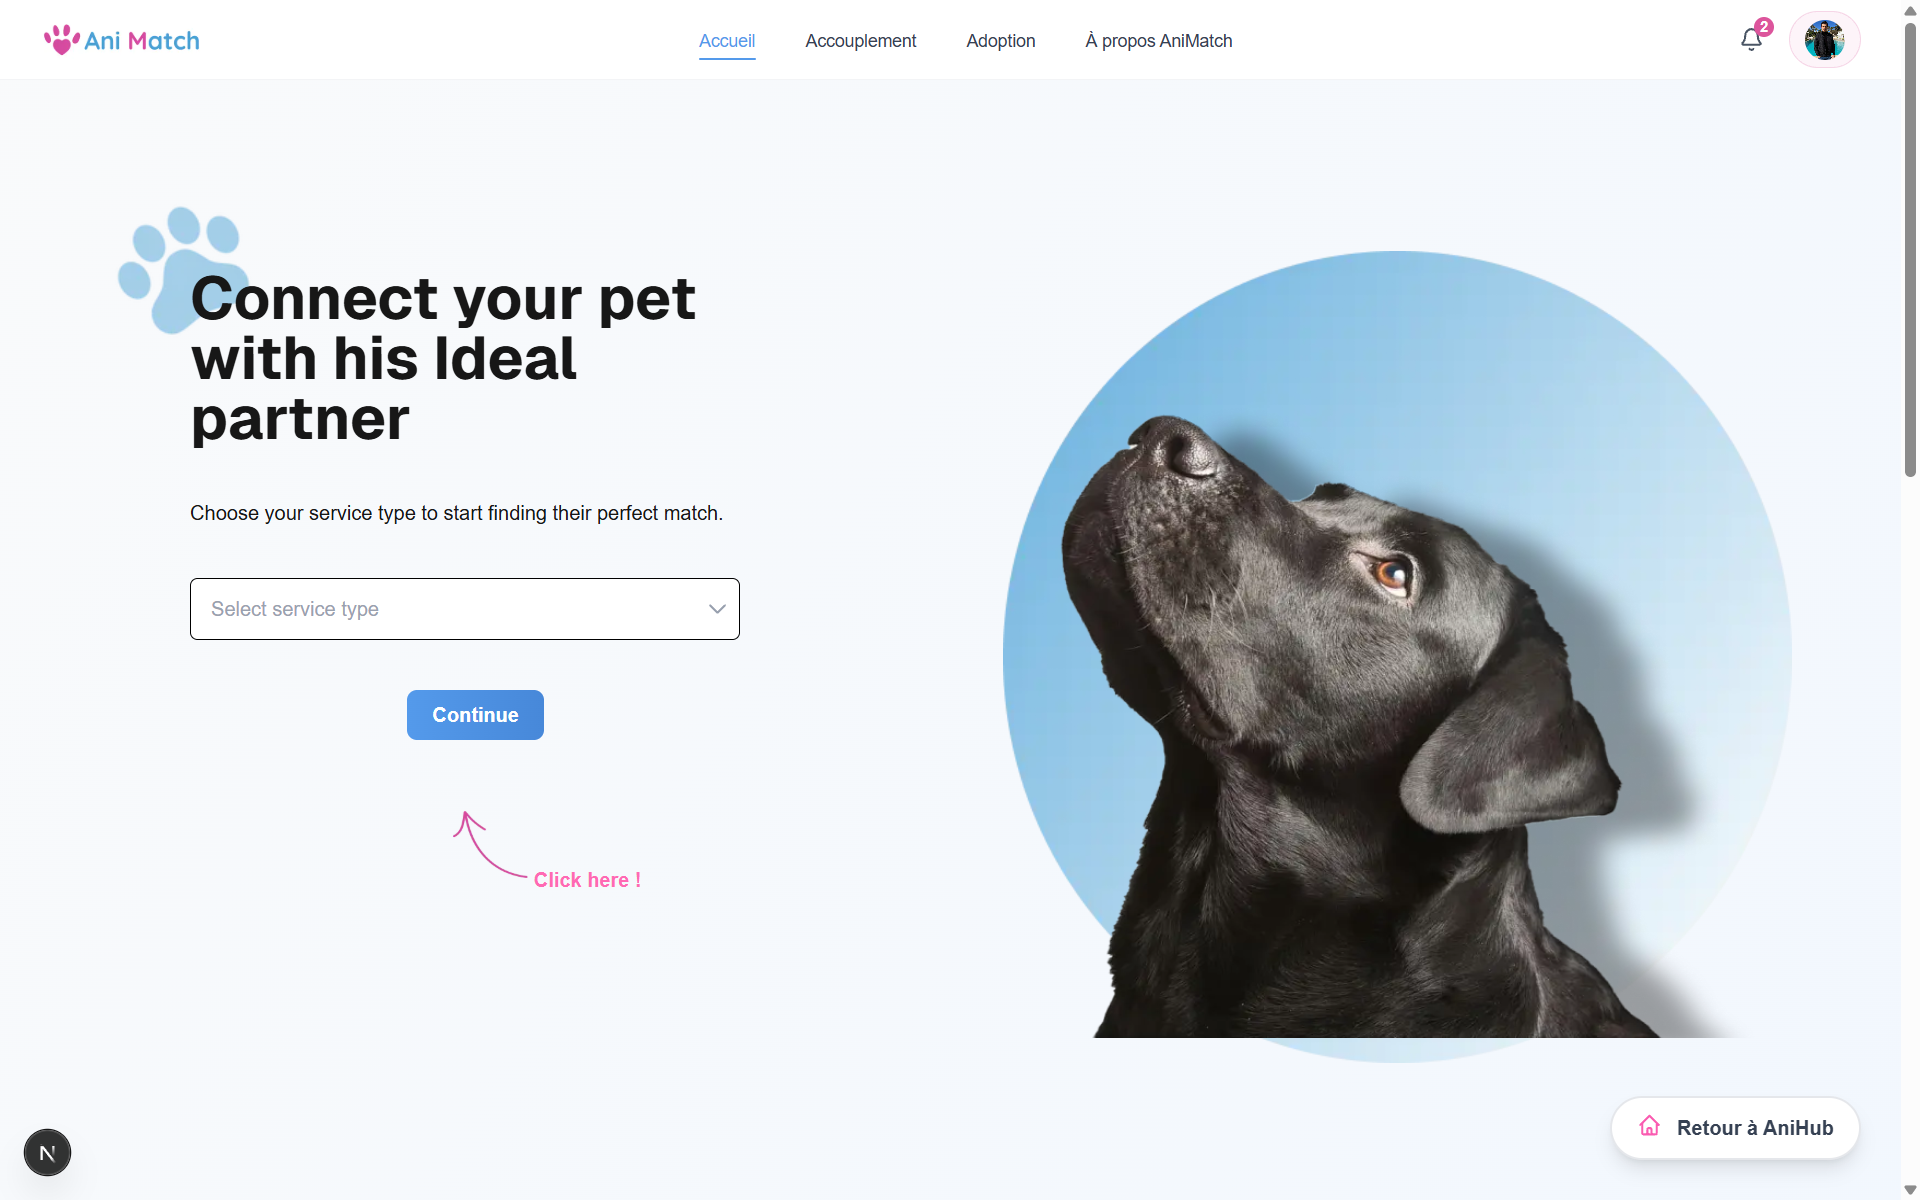
\includegraphics[width=0.8\textwidth]{images/acceuil animatch.png}
    \caption{Interface d’accueil du module AniMatch}
    \label{fig:acceuil_animatch}
\end{figure}   

\newpage

\subsubsection{Interface d’ajout d’une annonce d’accouplement}

La figure \ref{fig:ajout_annonce_accouplement} illustre l’interface permettant d’ajouter une annonce d’accouplement.

\begin{figure}[h!]
    \centering
    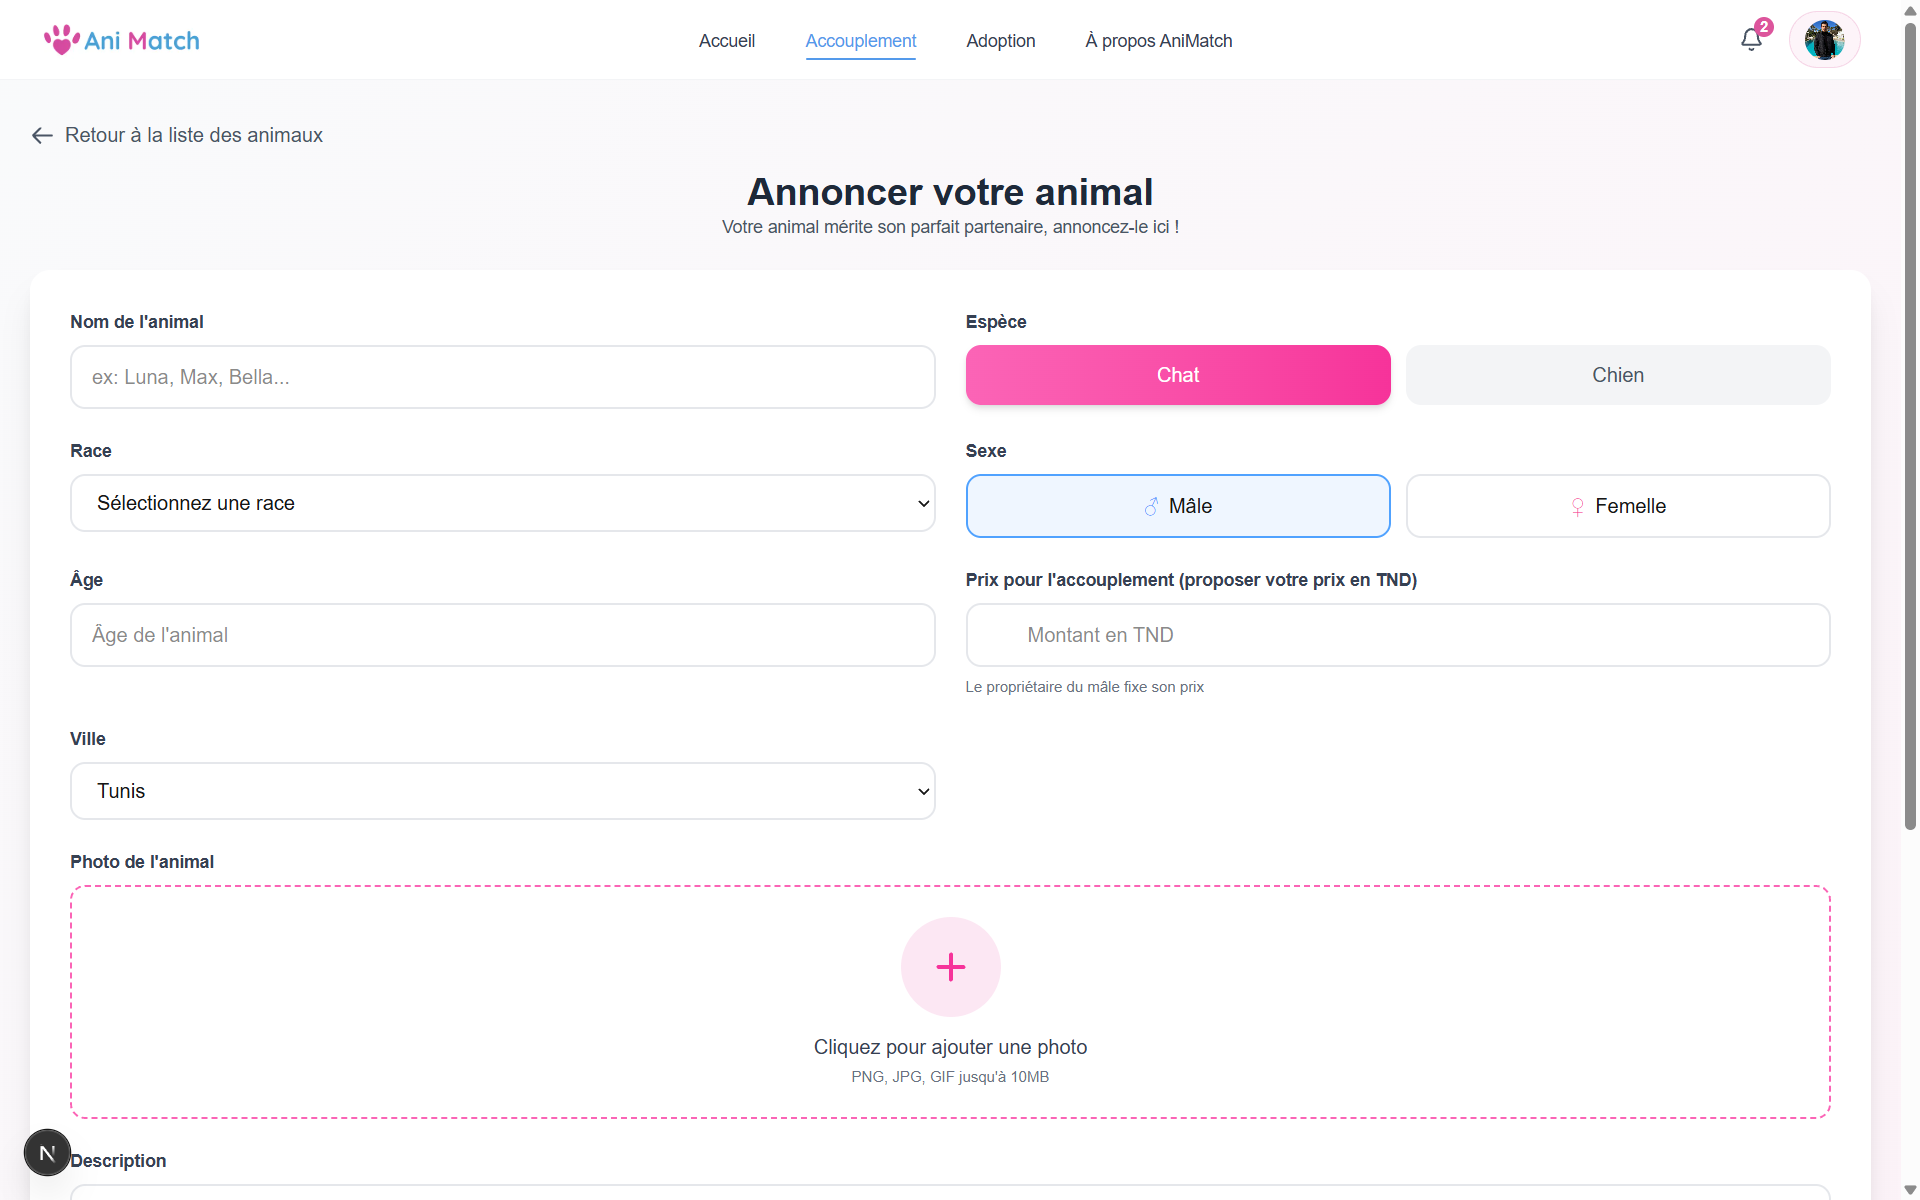
\includegraphics[width=0.74\textwidth]{images/ajouter animal accouplemnt.png}
    \caption{Interface d’ajout d’une annonce d’accouplement}
    \label{fig:ajout_annonce_accouplement}
\end{figure}

\subsubsection{Interface des animaux pour accouplement}

La figure \ref{fig:animaux_accouplement} illustre la liste des animaux disponibles pour l’accouplement.

\begin{figure}[h!]
    \centering
    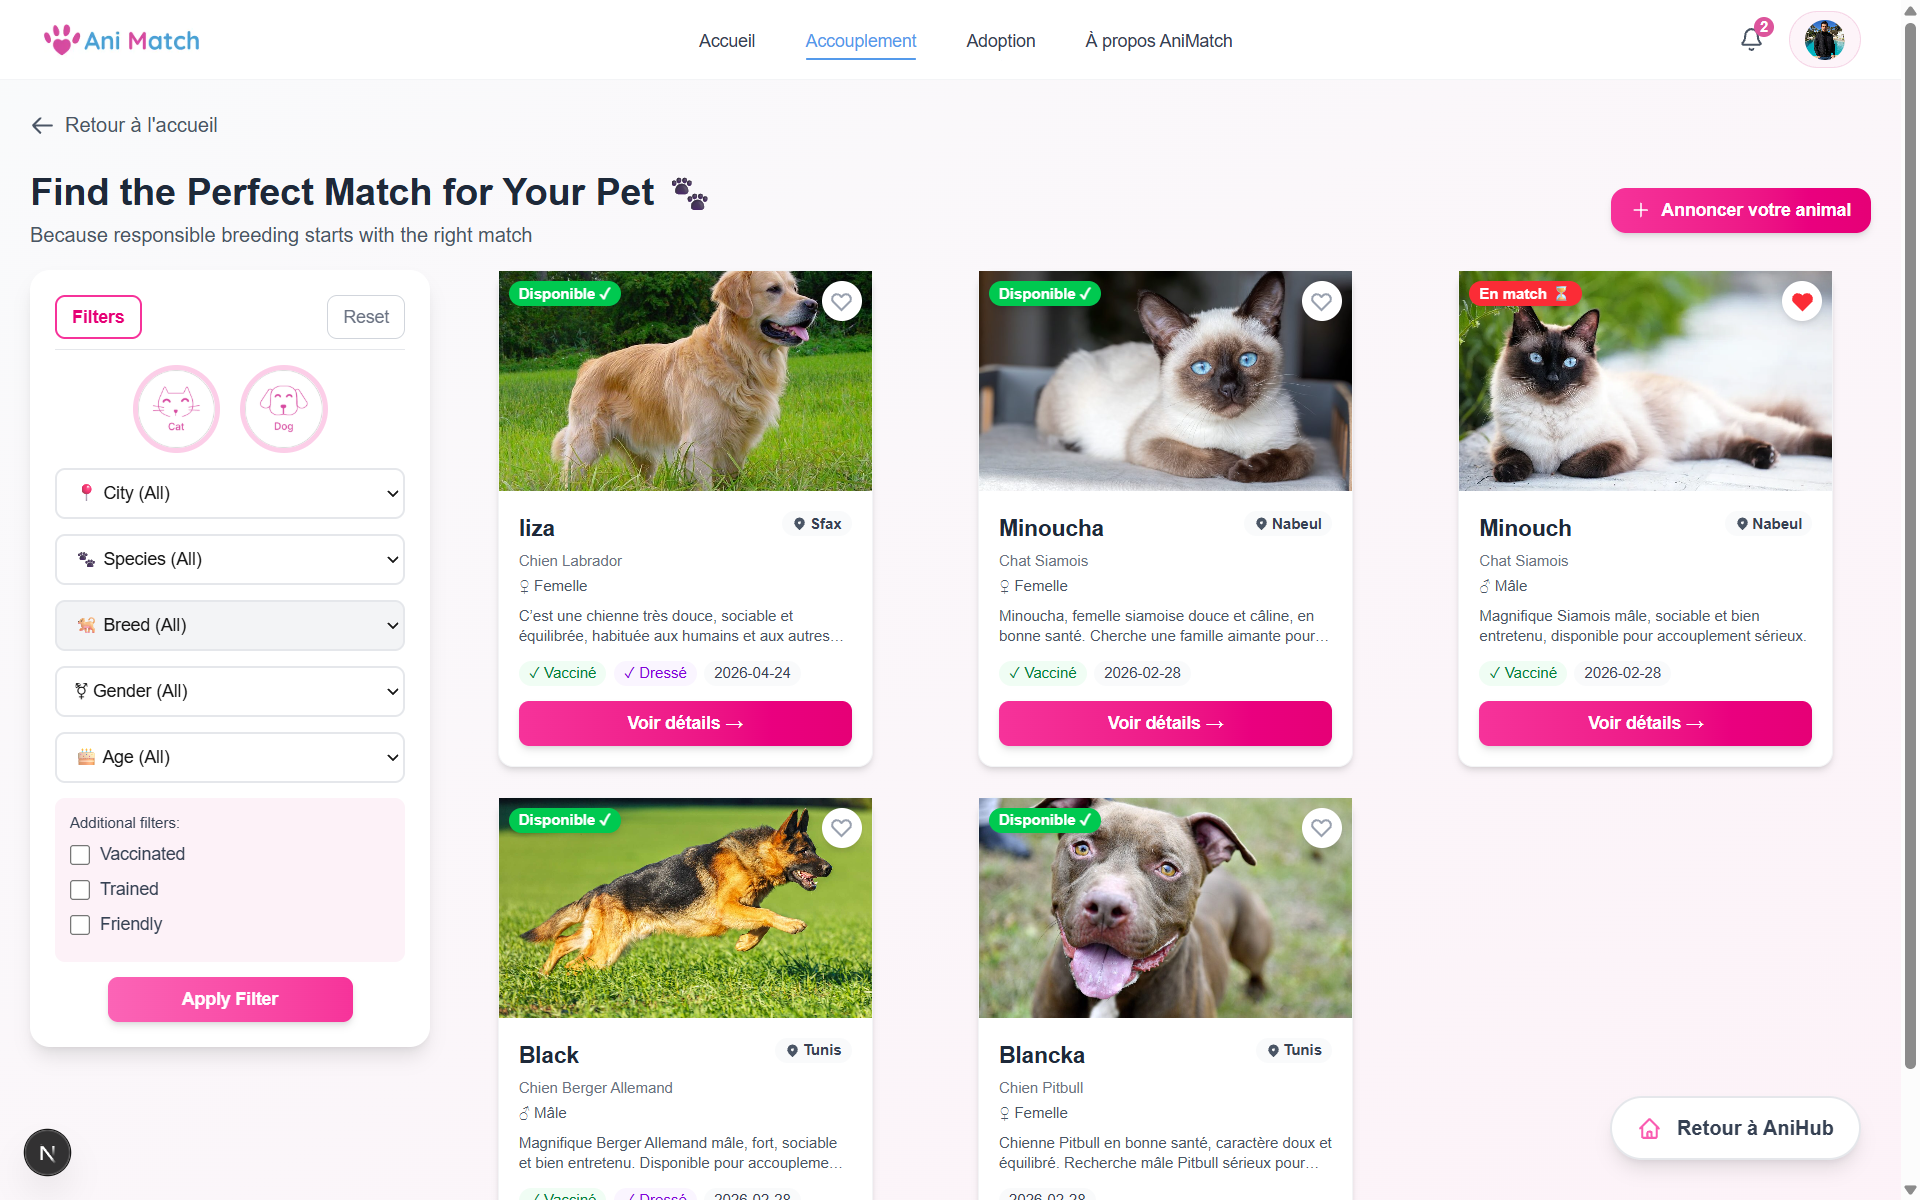
\includegraphics[width=0.74\textwidth]{images/animals accouplement.png}
    \caption{Interface des animaux pour accouplement}
    \label{fig:animaux_accouplement}
\end{figure}  

\newpage 

\subsubsection{Interface de détails d’une annonce d’accouplement}

La figure \ref{fig:details_annonce_accouplement} illustre les détails d’une annonce d’accouplement.

\begin{figure}[h!]
    \centering
    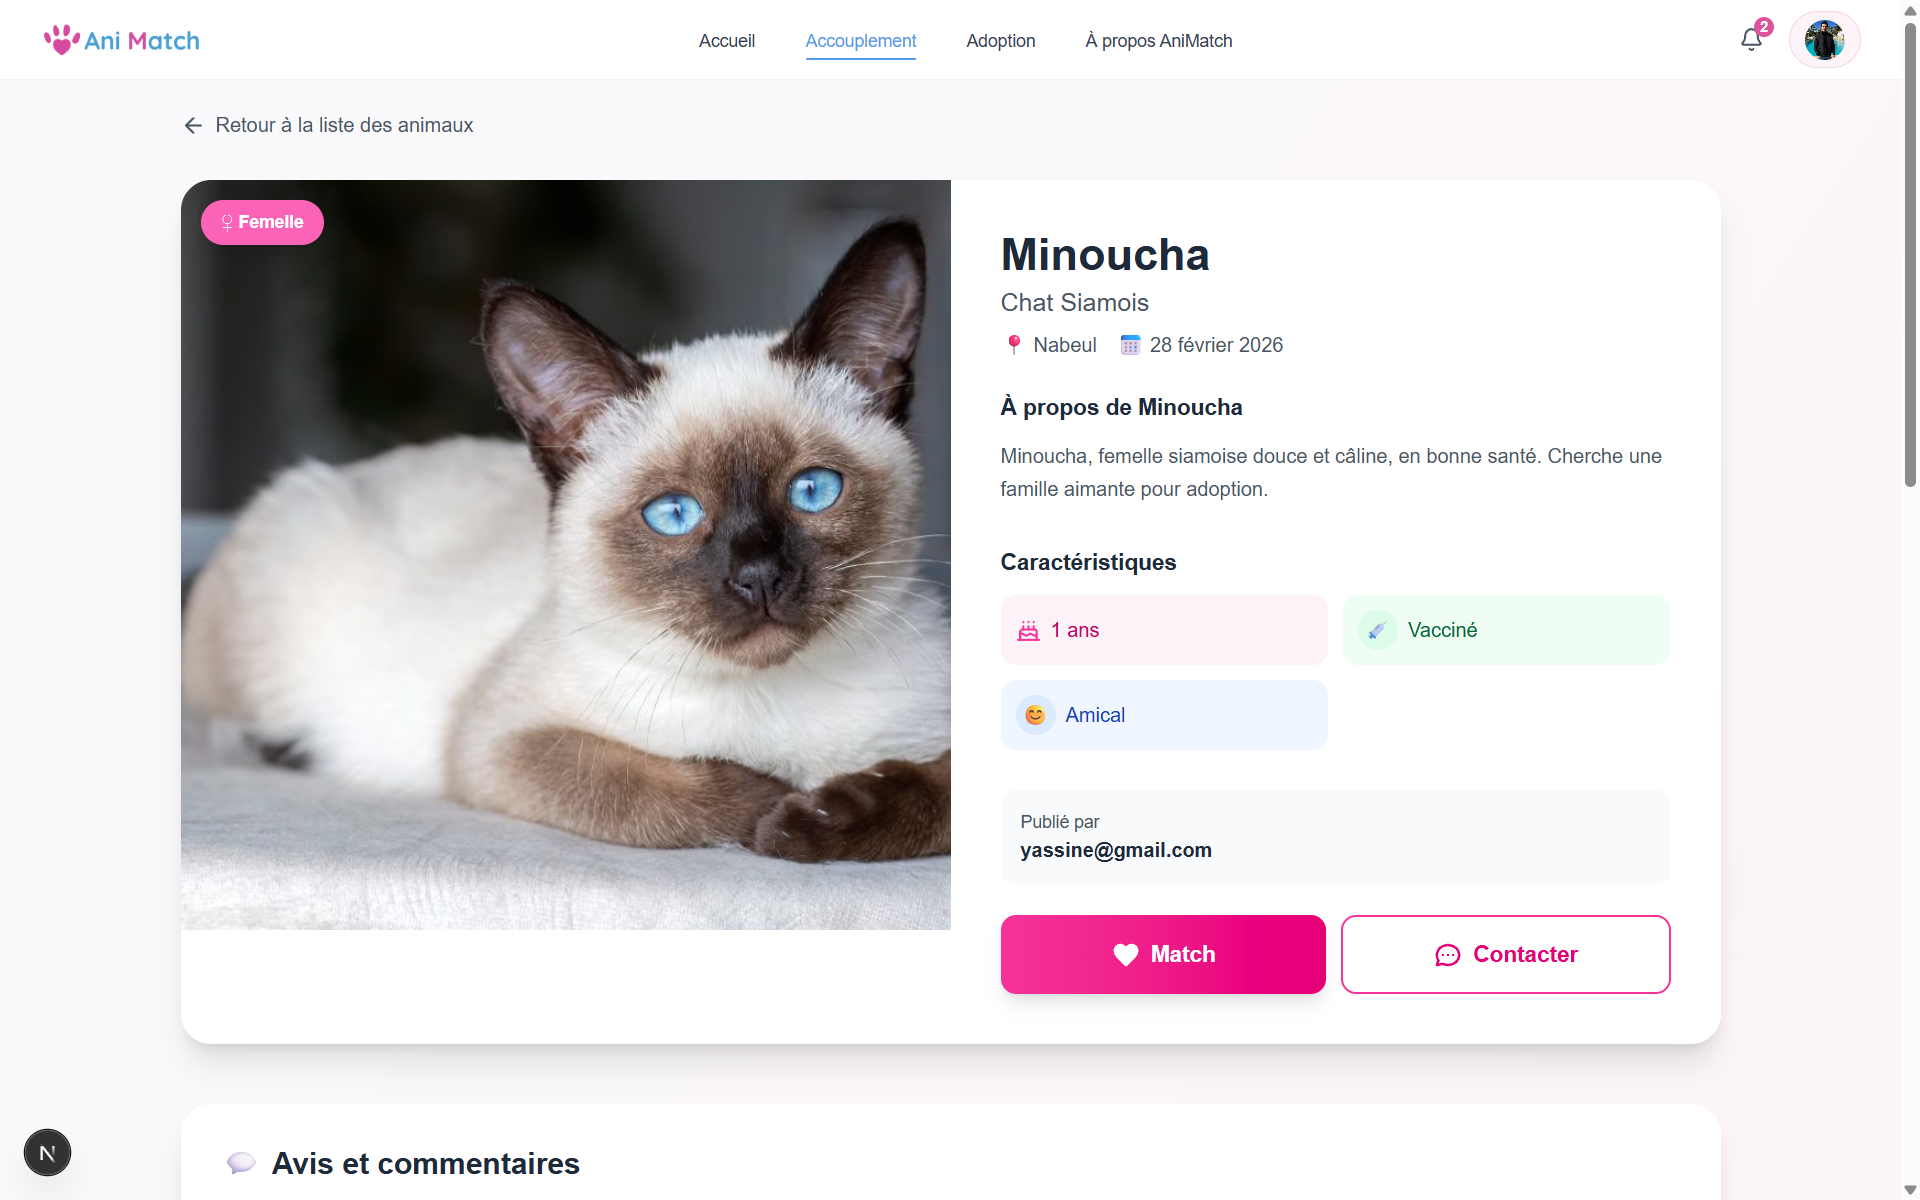
\includegraphics[width=0.72\textwidth]{images/detail.png}
    \caption{Interface de détails d’une annonce d’accouplement}
    \label{fig:details_annonce_accouplement}
\end{figure}

\subsubsection{Interface d’envoi d’une invitation d’accouplement}

La figure \ref{fig:envoyer_invitation_accouplement} illustre l’interface d’envoi d’une invitation à l’accouplement, permettant à l’utilisateur de rédiger un message et de l’envoyer au propriétaire de l’annonce.
\begin{figure}[h!]
    \centering
    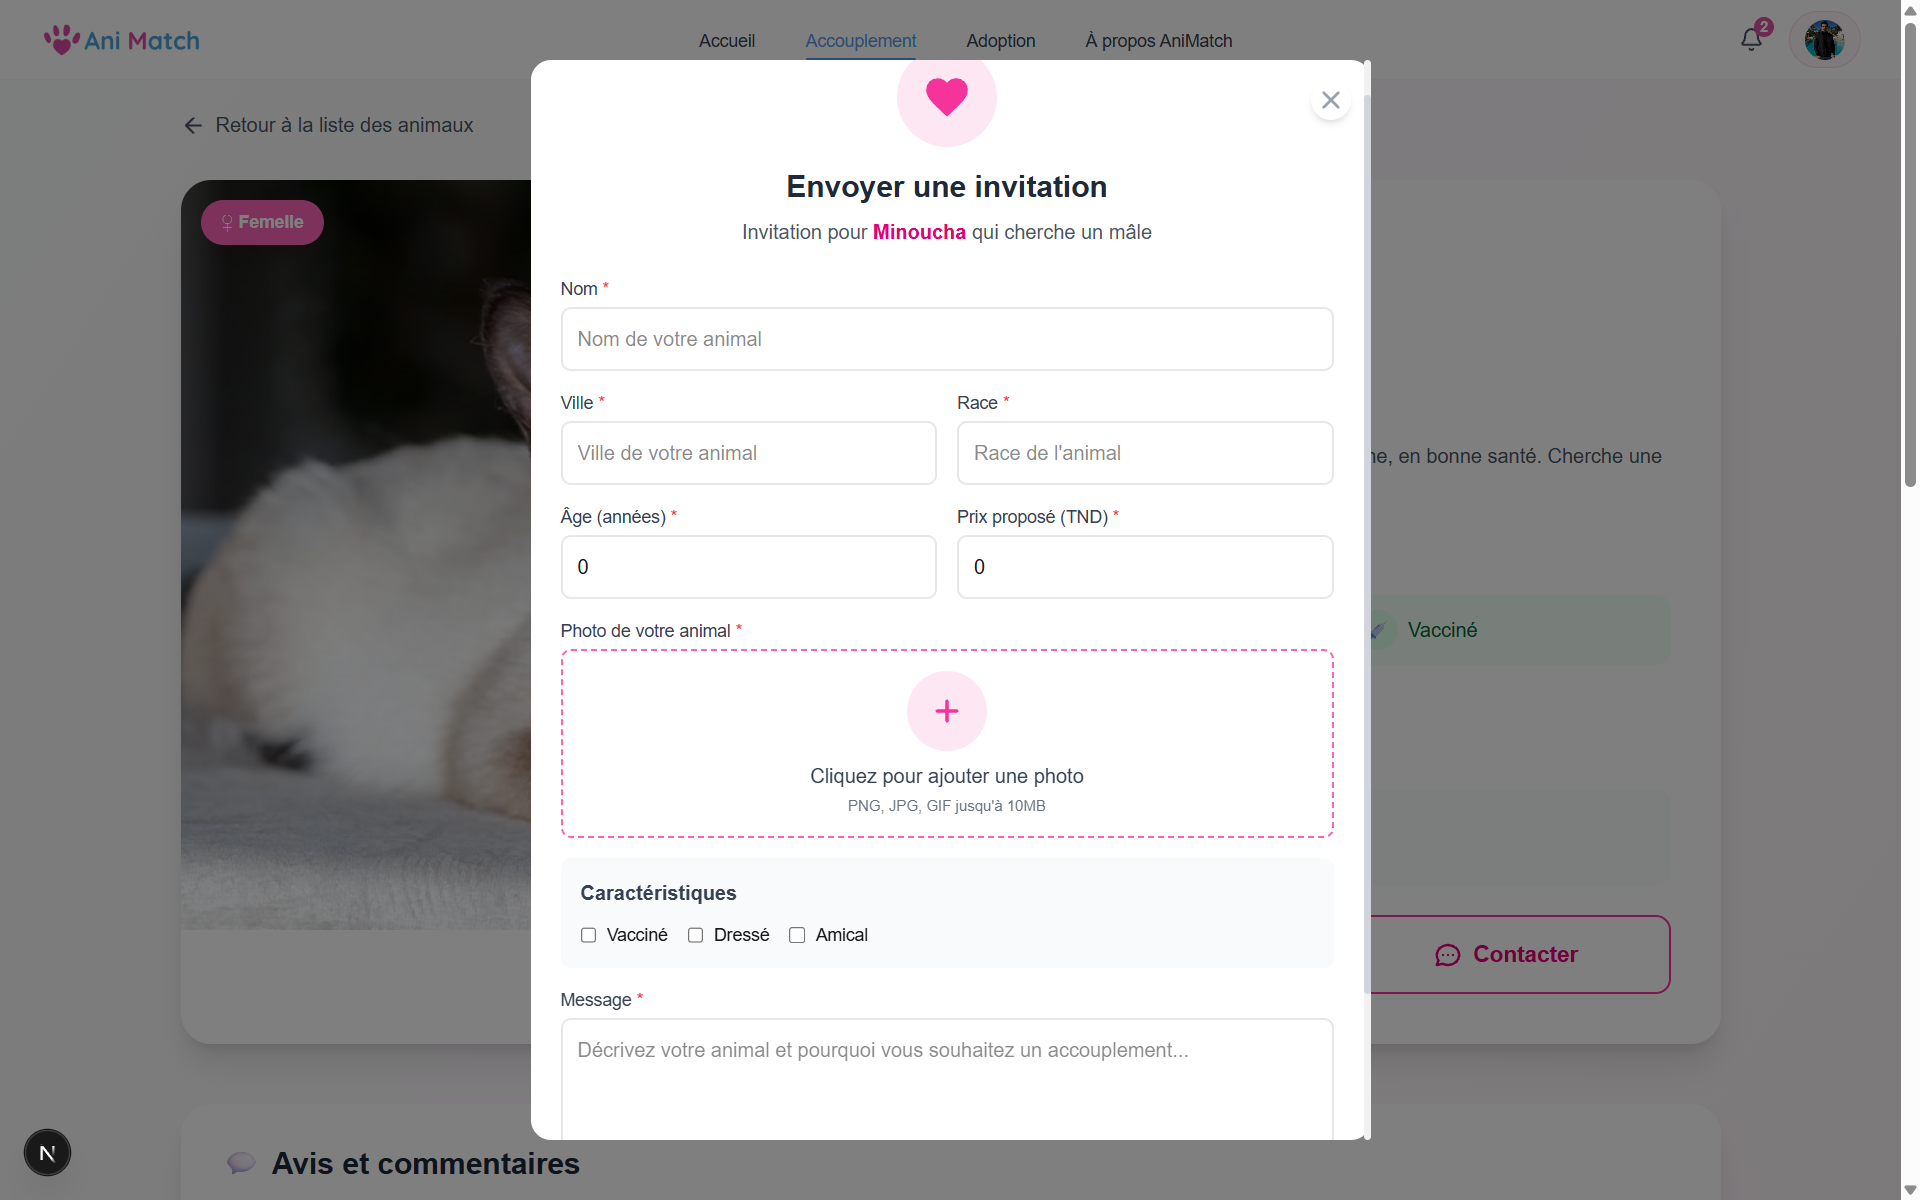
\includegraphics[width=0.72\textwidth]{images/envoyer invitation.png}
    \caption{Interface d’envoi d’une invitation à l’accouplement}
    \label{fig:envoyer_invitation_accouplement}
\end{figure} 

\newpage

\subsubsection{Interface des avis et commentaires}

La figure \ref{fig:avis_commentaires} illustre l’interface des avis et commentaires.

\begin{figure}[h!]
    \centering
    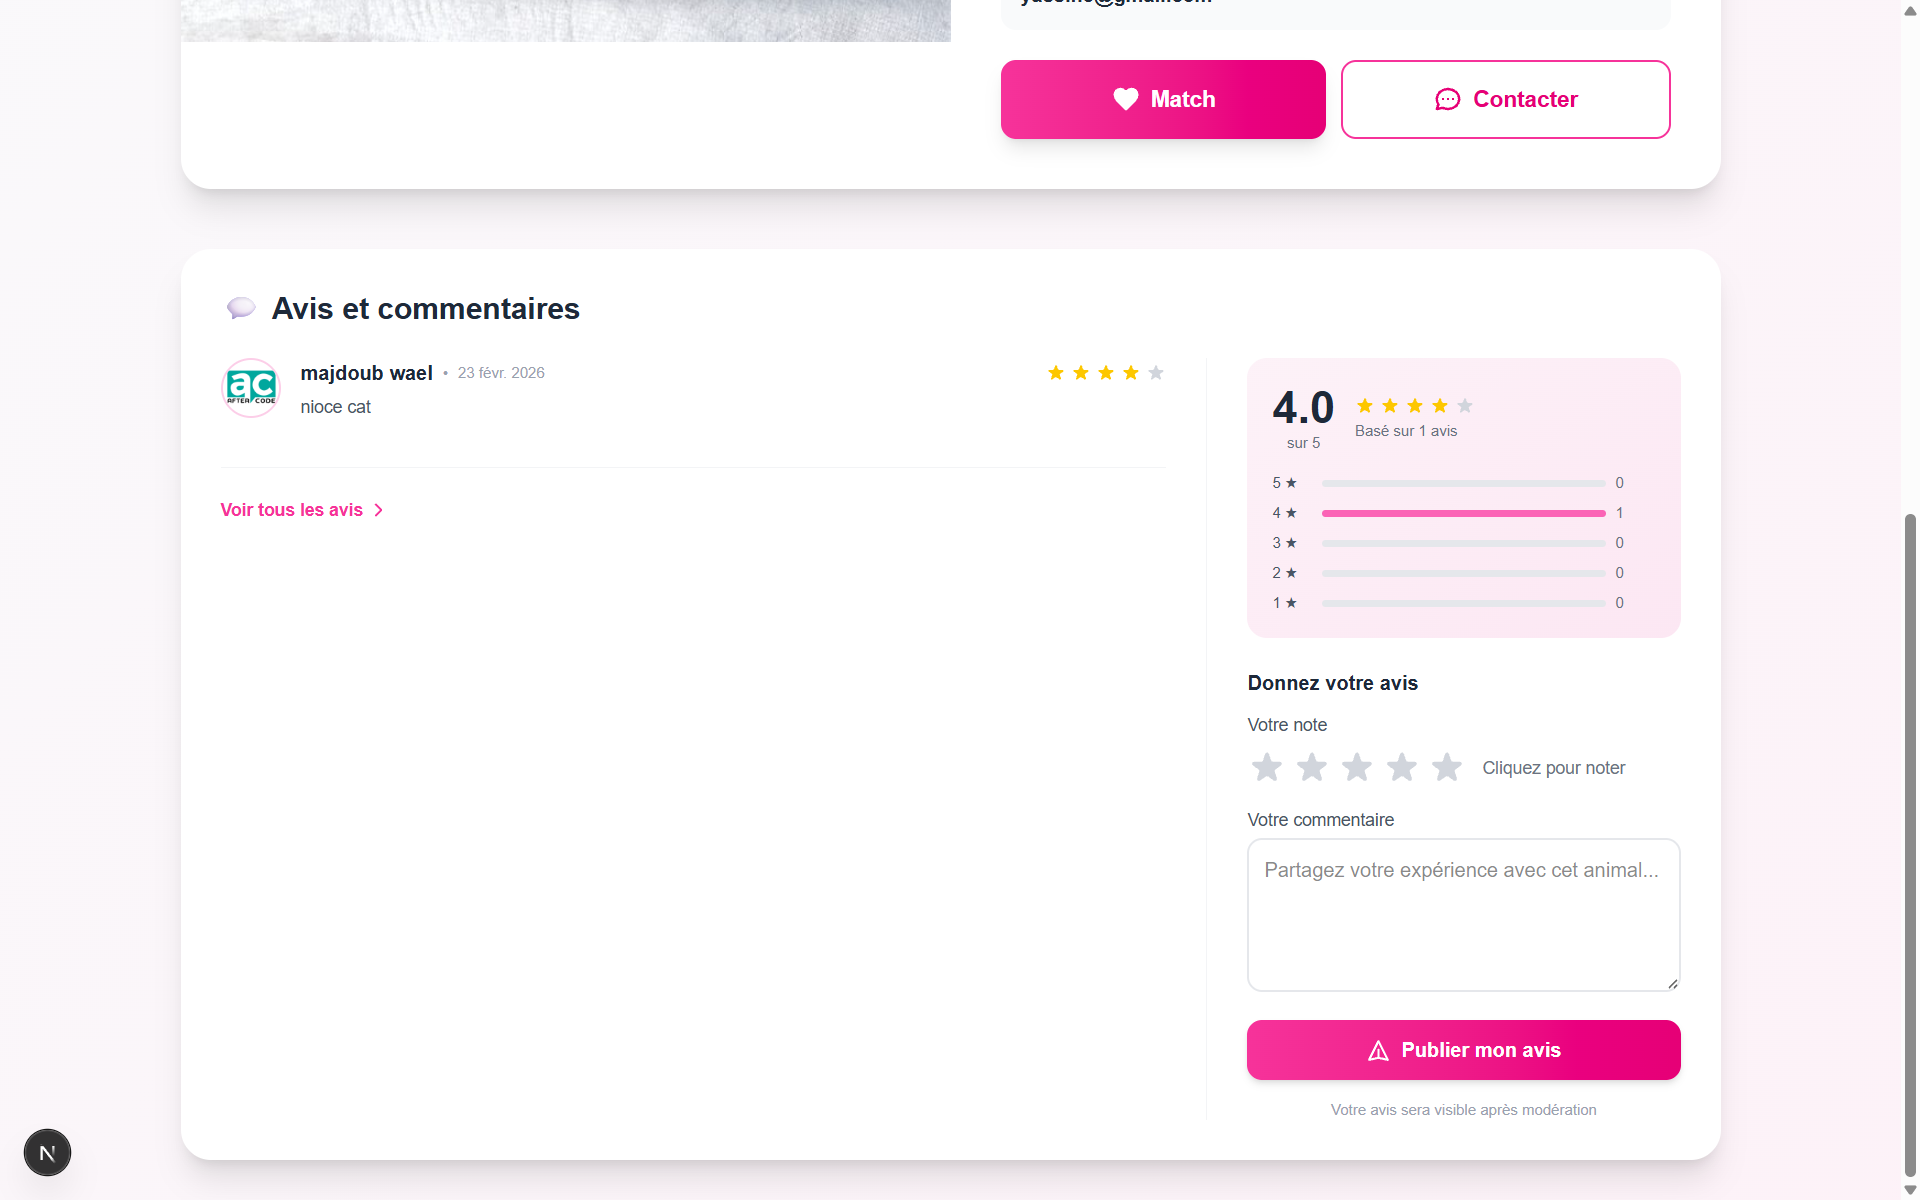
\includegraphics[width=0.74\textwidth]{images/comments section.png}
    \caption{Interface des avis et commentaires}
    \label{fig:avis_commentaires}
\end{figure} 

\subsubsection{Interface de gestion du profil}

La figure \ref{fig:gestion_profil} illustre l’interface de gestion du profil utilisateur dans son espace personnel « Espace AniMatch ». 
\begin{figure}[h!]
    \centering
    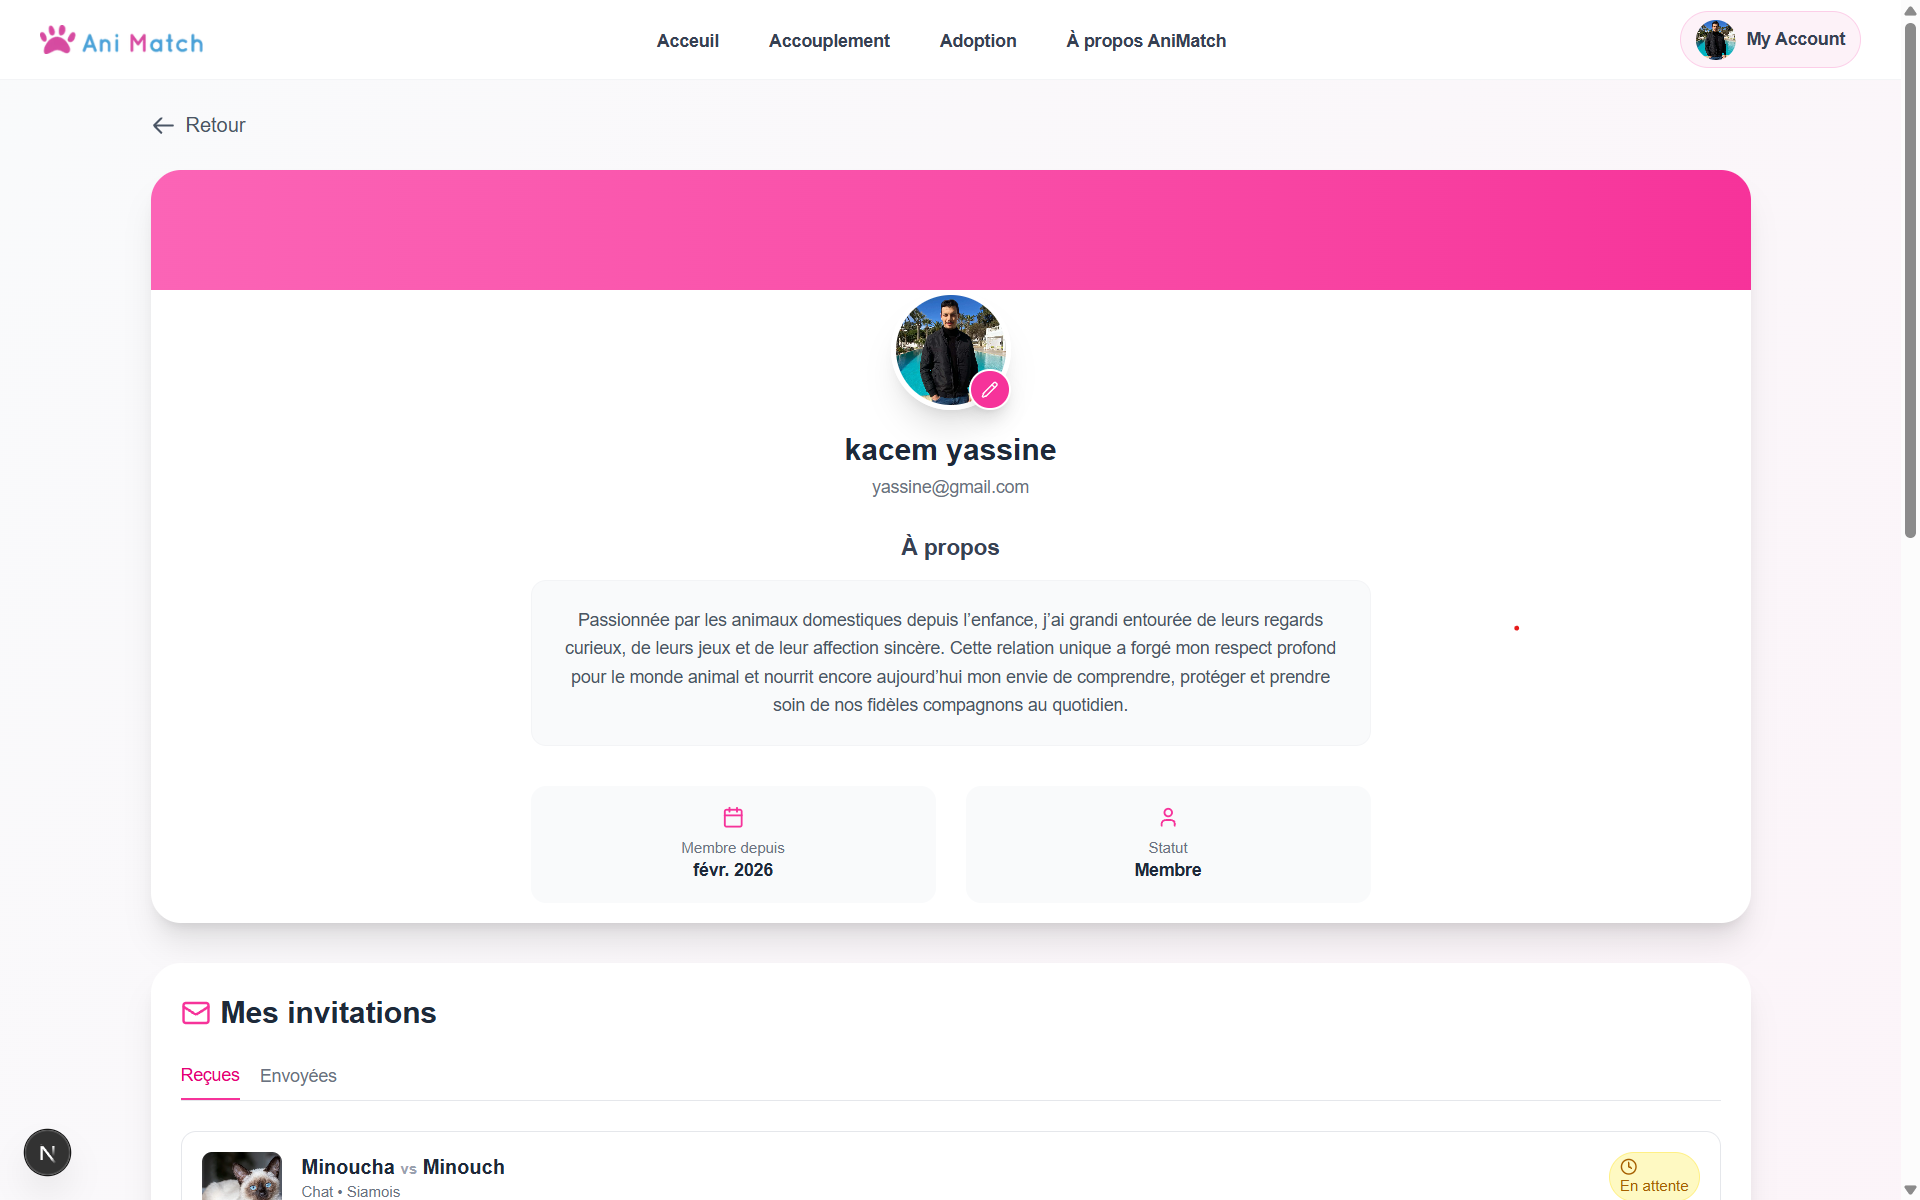
\includegraphics[width=0.74\textwidth]{images/profil page .png}
    \caption{Interface de gestion du profil utilisateur}
    \label{fig:gestion_profil}
\end{figure} 

\subsubsection{Interface de gestion de mes animaux (modification et suppression)} 

La figure \ref{fig:gestion_animaux_animatch} illustre l’interface de gestion des animaux permettant la modification et la suppression.

\begin{figure}[h!]
    \centering
    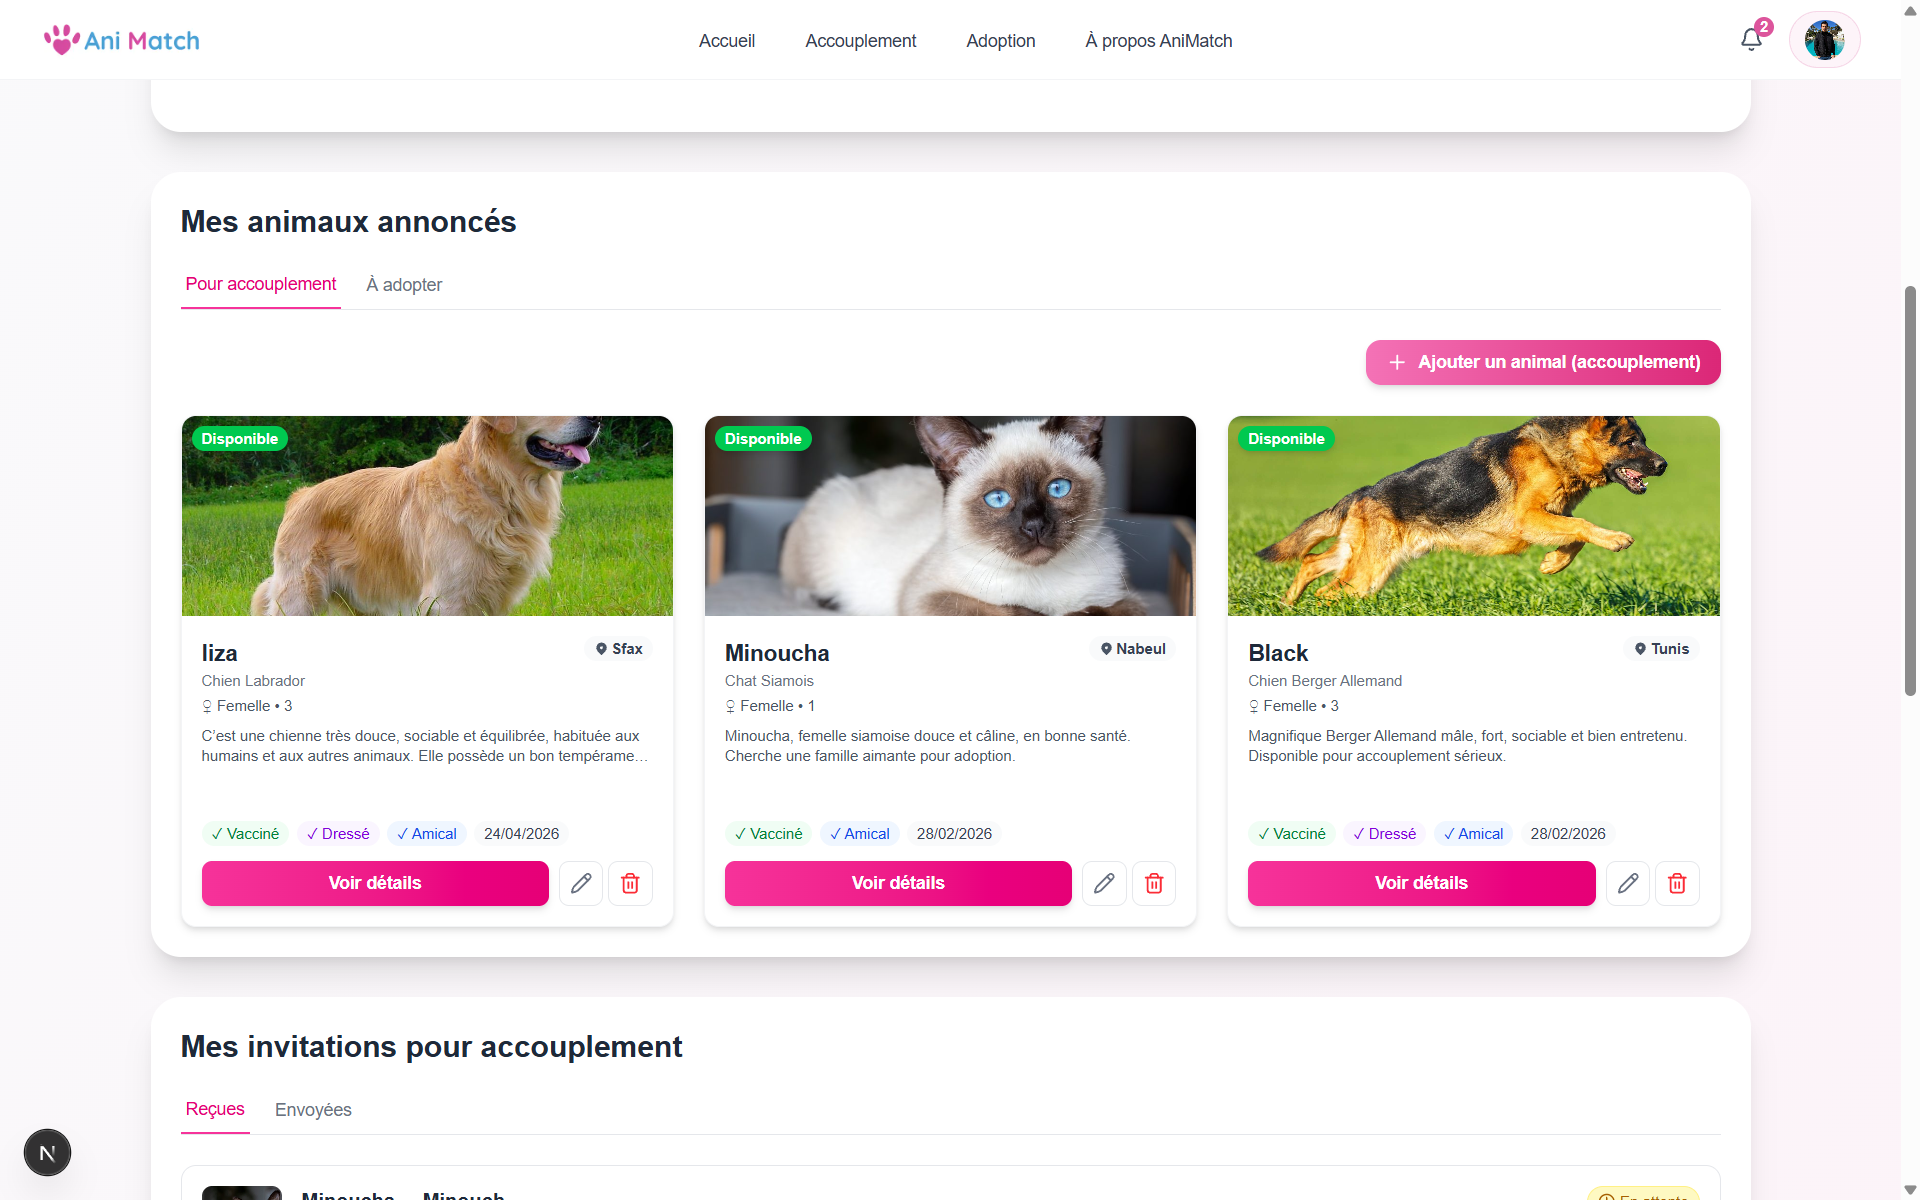
\includegraphics[width=0.74\textwidth]{images/profil page 2.png}
    \caption{Interface de gestion des animaux (modification et suppression)}
    \label{fig:gestion_animaux_animatch}
\end{figure}

\subsubsection{Interface de gestion de mes invitations pour adoption reçues} 

La figure \ref{fig:invitations_adoption_recues} illustre l’interface de gestion des invitations d’adoption reçues.

\begin{figure}[h!]
    \centering
    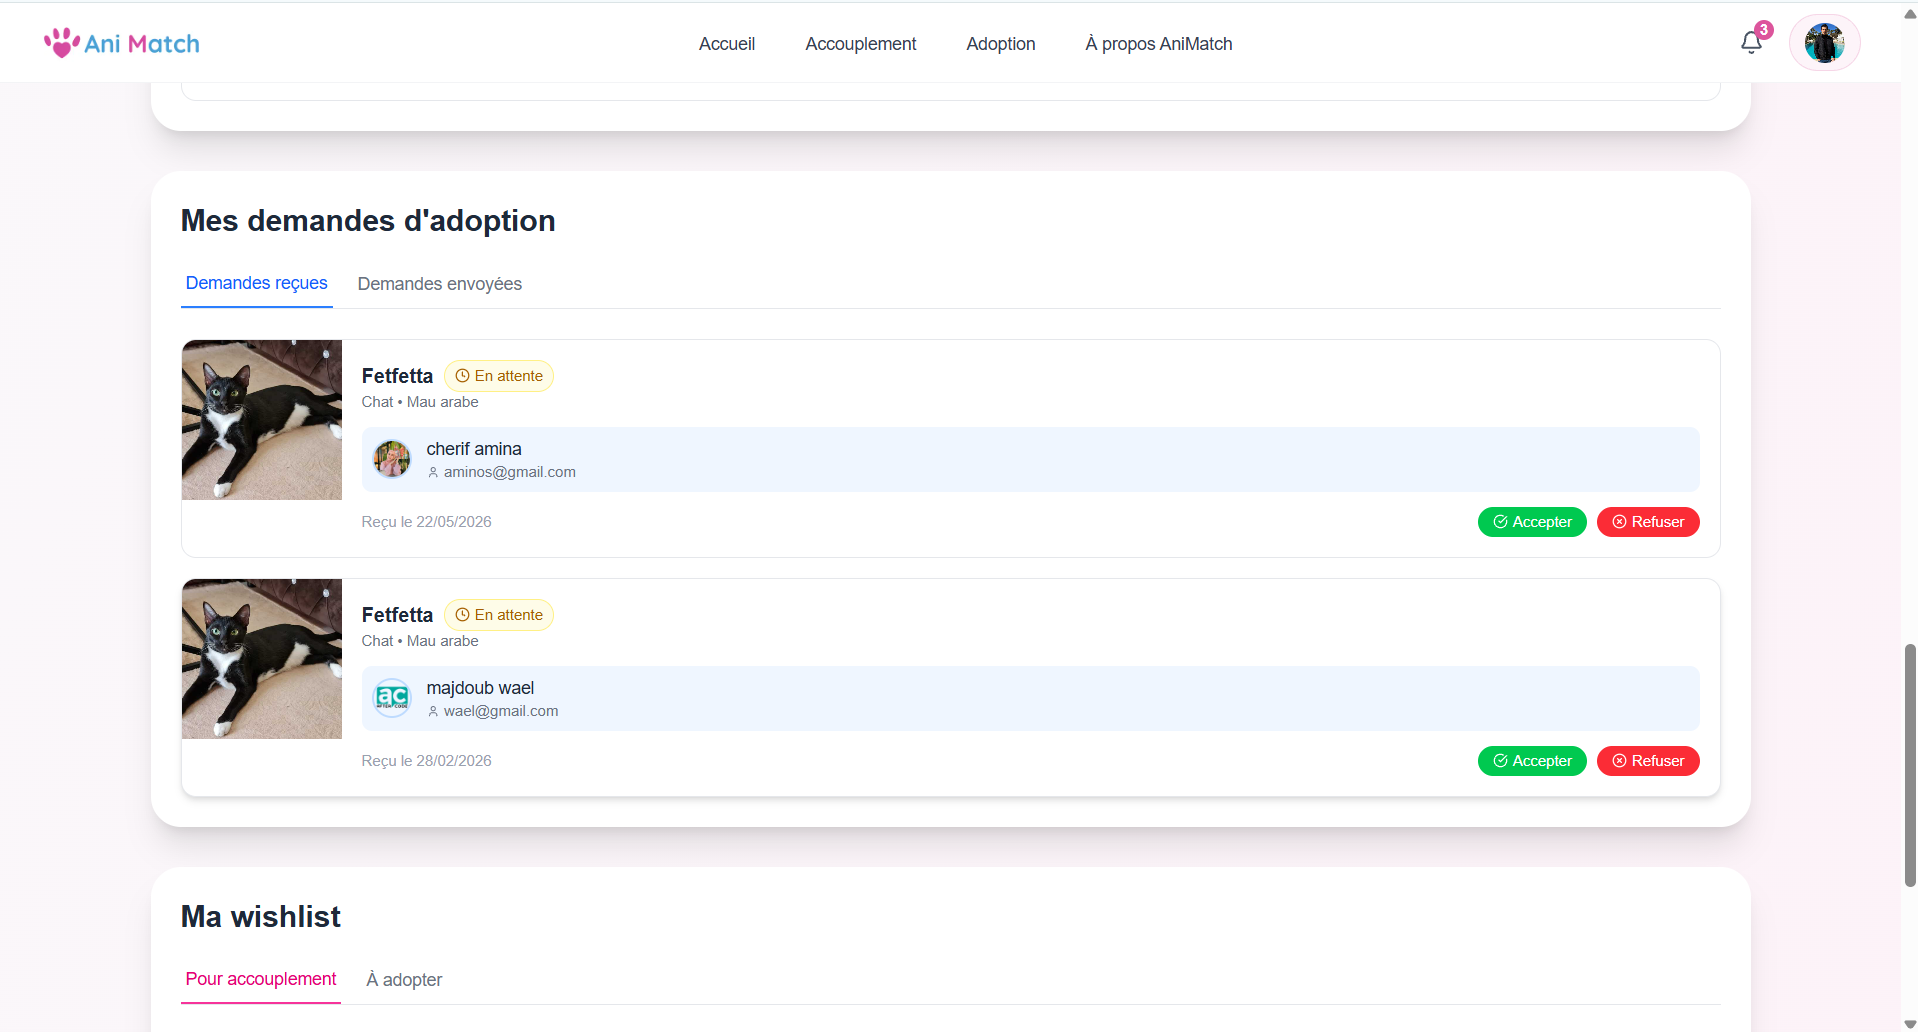
\includegraphics[width=0.85\textwidth]{images/mes demandes d adoption recus.png}
    \caption{Interface de gestion des invitations d’adoption reçues}
    \label{fig:invitations_adoption_recues}
\end{figure}

\newpage 

\subsubsection{Interface de gestion de mes invitations pour accouplement reçues}

La figure \ref{fig:invitations_accouplement_recues} illustre l’interface de gestion des invitations d’accouplement reçues.

\begin{figure}[h!]
    \centering
    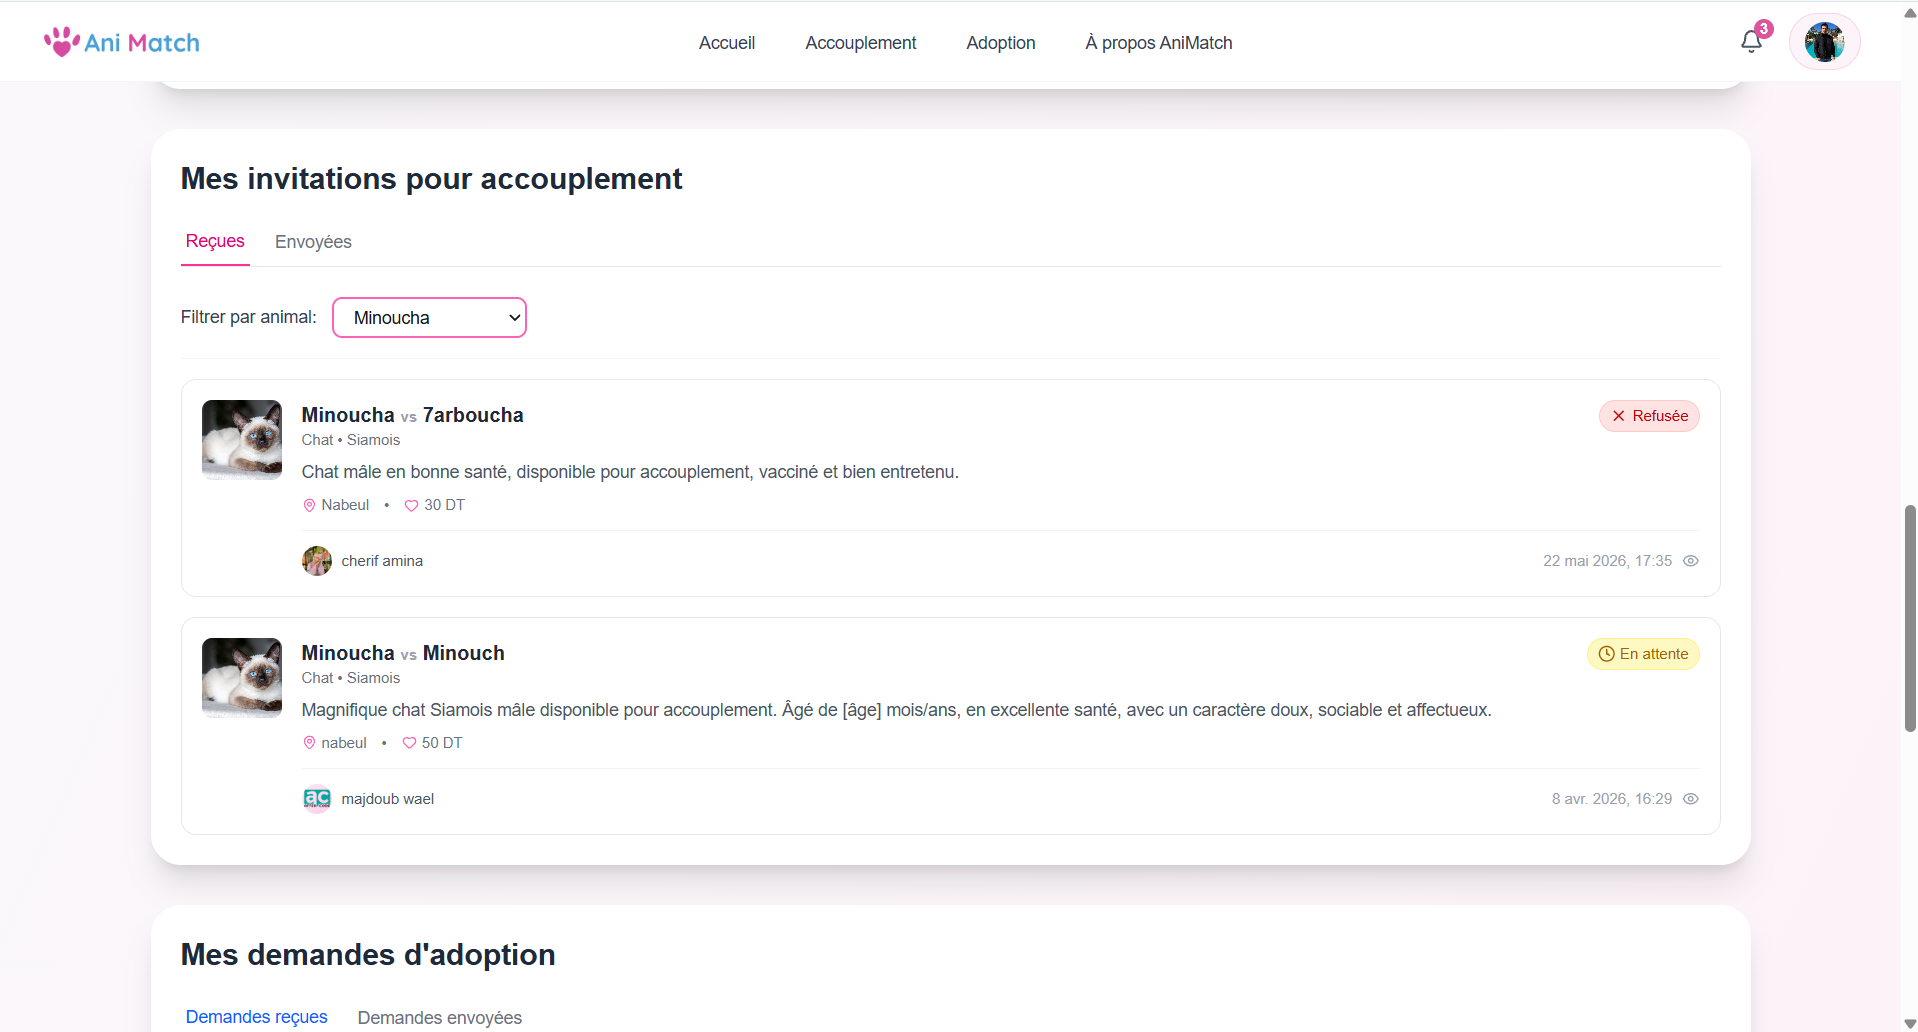
\includegraphics[width=0.85\textwidth]{images/mes invitations pour accouplements recus.png}
    \caption{Interface de gestion des invitations d’accouplement}
    \label{fig:invitations_accouplement_recues}
\end{figure} 

\subsubsection{Interface de détails d’une invitation d’accouplement reçue}

La figure \ref{fig:details_invitation_accouplement} illustre les détails d’une invitation d’accouplement reçue.

\begin{figure}[h!]
    \centering
    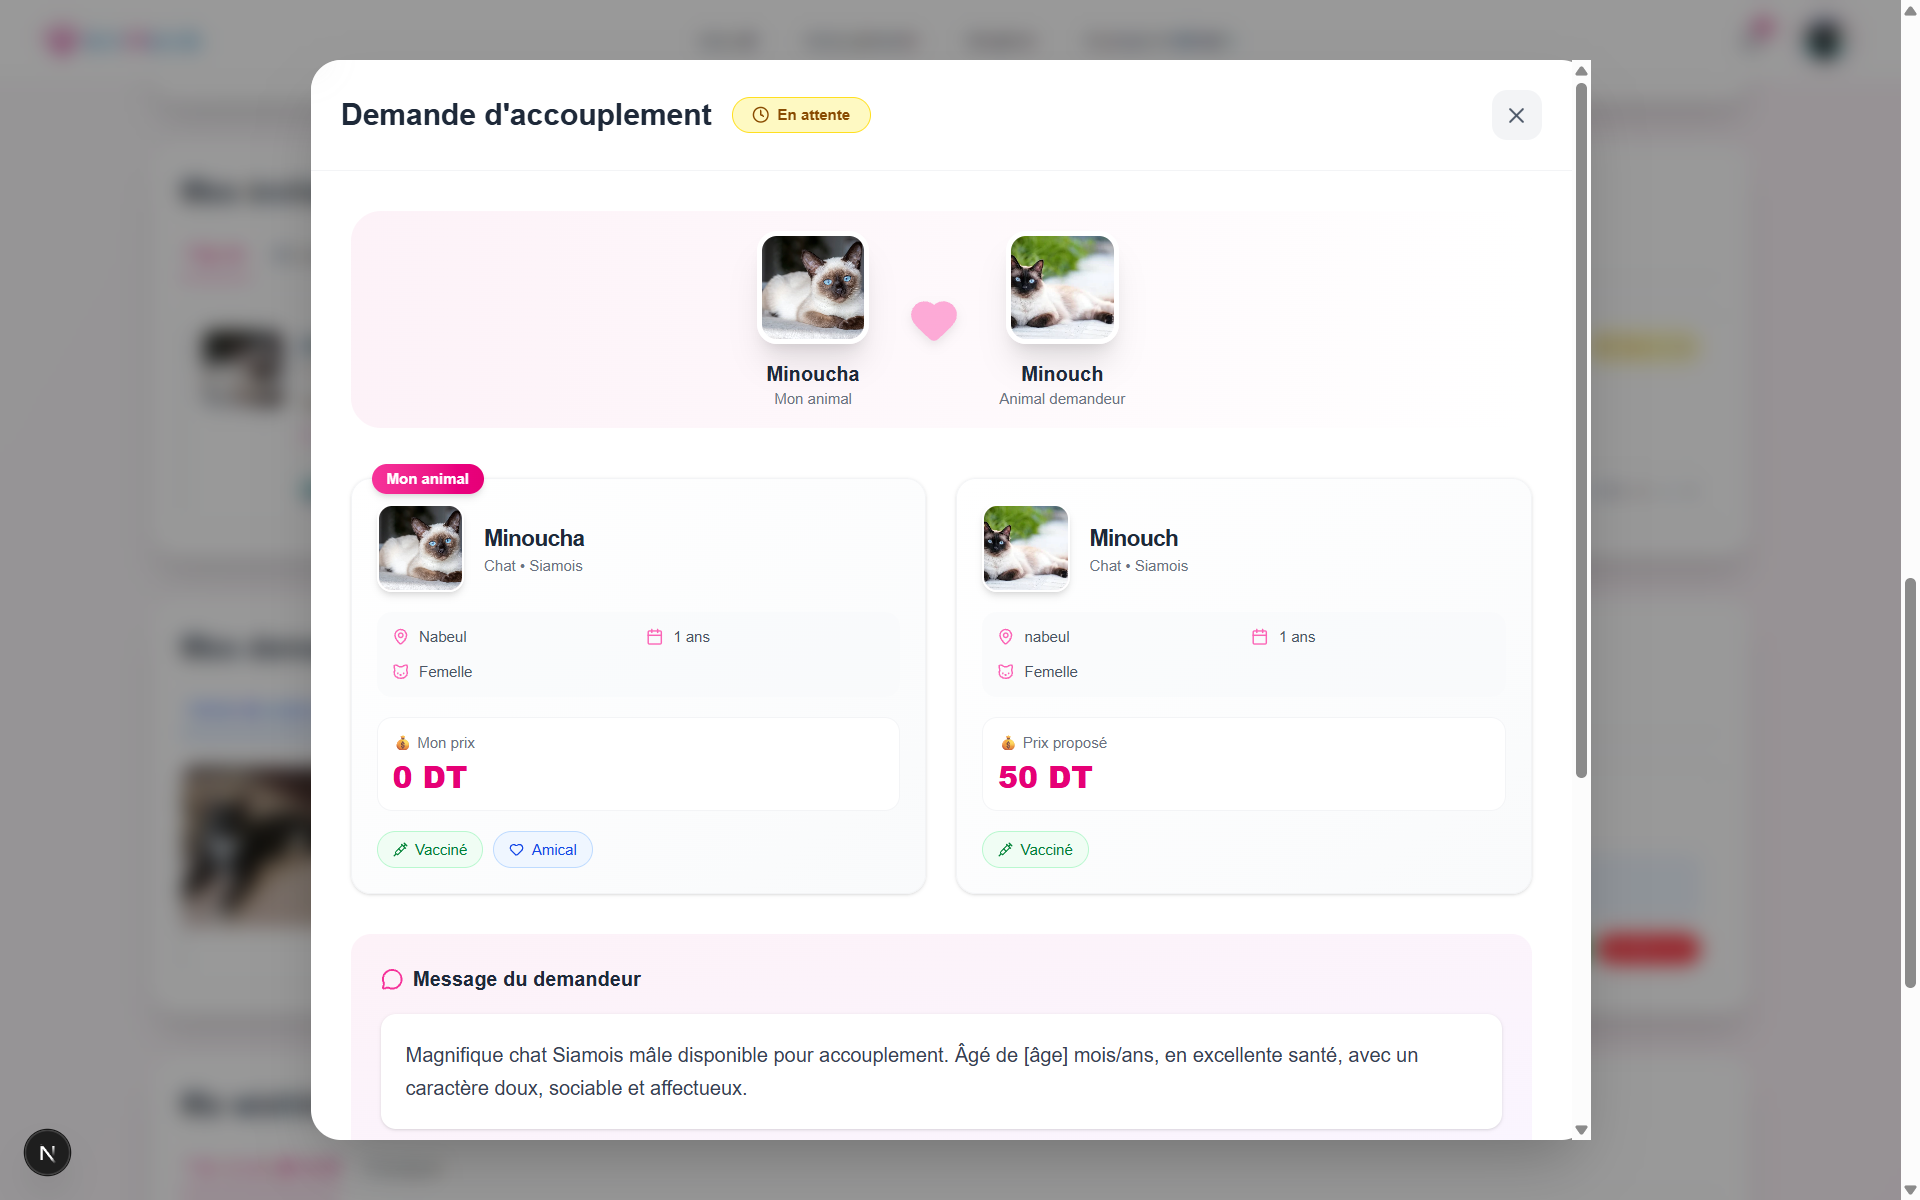
\includegraphics[width=0.8\textwidth]{images/invi recu 1.png}
    \caption{Interface de détails d’une invitation d’accouplement}
    \label{fig:details_invitation_accouplement}
\end{figure}

\newpage\section{Sprint 3 : Module AniFound}
La figure \ref{fig:logo-anifound} illustre le logo du module AniFound.

\begin{figure}[h!]
    \centering
    
\includegraphics[width=3.5cm]{images/Logo anifound.png}
    \caption{Logo du module AniFound}
    \label{fig:logo-anifound}
\end{figure}

Ce sprint de \textbf{3 semaines} est consacré au module AniFound, dédié à la déclaration et la gestion des animaux trouvés, ainsi qu’à leur restitution à leurs propriétaires.
\subsection{Sprint backlog}  
La table \ref{tab:sprint3-backlog} présente le Sprint Backlog du sprint 3 avec les user stories, les tâches associées et les efforts estimés :
\begin{longtable}{|p{2cm}|p{5cm}|p{6cm}|p{2cm}|}
\caption{Sprint Backlog du sprint 3 }
\label{tab:sprint3-backlog} \\ 
\hline
\rowcolor{coloranifound}
\textbf{ID} & \textbf{User Story} & \textbf{Tâches} & \textbf{Effort} \\
\hline
\endfirsthead

\hline
\rowcolor{coloranifound}
\textbf{ID} & \textbf{User Story} & \textbf{Tâches} & \textbf{Effort} \\
\hline
\endhead

% ===================== US1 =====================
\multirow{8}{2cm}{US1}
& \multirow{8}{5cm}{En tant qu’utilisateur, je souhaite consulter les déclarations de perte et de trouvaille afin de retrouver ou identifier un animal}
& Conception de maquette Figma & 0.5 j \\
\cline{3-4}
& & API récupération déclarations & 0.5 j \\
\cline{3-4}
& & Filtrage, tri et recherche des déclarations & 1 j \\
\cline{3-4}
& &Pagination & 1 j \\
\cline{3-4}
& & Enregistrer une déclaration à consulter ultérieurement & 0.5 j \\ 
\cline{3-4}
& & Intégration frontend/backend & 1 j \\
\cline{3-4}
& & Flouter les déclarations de trouvaille pour préserver la confidentialité & 0.5 j \\ 
\cline{3-4}
& & Tests & 0.5 j \\
\hline

% ===================== US2 =====================
\multirow{9}{2cm}{US2}
& \multirow{9}{5cm}{En tant qu’utilisateur, je veux gérer mes déclarations de perte et de trouvaille afin de les publier, les consulter, les modifier ou les supprimer.}
& Conception de maquette Figma & 0.5 j \\
\cline{3-4}
& & APIs création,mise à jour et déclaration & 1 j \\
\cline{3-4}
& & Upload image Cloudinary & 0.5 j \\
\cline{3-4}
& & Intégration avec MS Auth (JWT) & 0.5 j \\
\cline{3-4}
& & Intégration frontend/backend & 1 j \\ 
\cline{3-4}
& & Tests & 0.5 j \\    
\hline

% ===================== US3 =====================
\multirow{6}{2cm}{US3}
& \multirow{6}{5cm}{En tant qu’utilisateur, je veux envoyer un indice afin de prouver qu’il s’agit bien de mon animal.}
& Conception figma de l'interface envoi & 0.5 j \\
\cline{3-4}
& & API envoi indice & 1 j \\
\cline{3-4}
& & Upload image de l'indice dans Cloudinary & 0.5 j \\
\cline{3-4}
& & Intégration avec MSAuth (JWT) & 0.5 j \\
\cline{3-4}
& & Tests & 0.5 j \\
\hline

% ===================== US4 =====================
\multirow{5}{2cm}{US}
& \multirow{5}{5cm}{En tant qu’utilisateur, je veux gérer les indices reçus afin de les examiner et d’y répondre (acceptation ou refus)}
 & Conception de maquette Figma pour l'interface des indices reçus & 0.5 j \\
\cline{3-4}
& & API d’acceptation et de refus des indices & 1 j \\
\cline{3-4}
& & Intégration avec MSAuth (JWT)  & 0.5 j \\
\cline{3-4} 
& & Intégration frontend/backend   & 0.5 j \\
\cline{3-4} 
& & Tests & 0.5 j \\
\hline

% ===================== US5 =====================
\multirow{8}{2cm}{US5}
& \multirow{8}{5cm}{En tant qu’utilisateur, je veux gérer mes notifications afin d’être informé des interactions sur mes déclarations}
& Analyse besoins notifications & 0.5 j \\
\cline{3-4}
& & Développement microservice Notifications & 1 j \\
\cline{3-4}
& & Intégration RabbitMQ avec AniFound & 1 j \\
\cline{3-4}
& & Intégration RabbitMQ Notifications & 1 j \\
\cline{3-4}
& & Création événements (indices, validation, etc.) & 0.5 j \\
\cline{3-4}
& & Interface notifications frontend & 0.5 j \\
\cline{3-4}
& & Marquer comme lu / non lu & 0.5 j \\
\cline{3-4}
& & Tests & 0.5 j \\
\hline

% ===================== US6 =====================
\multirow{4}{2cm}{US6}
& \multirow{4}{5cm}{En tant qu’utilisateur, je veux contacter l’autre partie afin d’échanger des informations et faciliter la résolution de la situation.}
& Analyse & 0.5 j \\
\cline{3-4}
& & Intégration bouton WhatsApp & 0.5 j \\
\cline{3-4}
& & Génération lien wa.me & 0.5 j \\
\cline{3-4}
& & Tests & 0.5 j \\
\hline

\end{longtable}
\newpage 

\subsection{Diagramme des cas d’utilisation du sprint 3}
Dans cette section, nous présentons le diagramme des cas d’utilisation du sprint dédié au module \textbf{AniFound}. 

Ce diagramme illustre les principales interactions entre l’utilisateur et le système, notamment la déclaration des animaux perdus ou trouvés, la consultation des annonces, la gestion des déclarations, l’échange d’indices ainsi que la communication entre les utilisateurs afin de faciliter la restitution des animaux.

La figure \ref{fig:usecase-sprint3} représente le diagramme des cas d’utilisation correspondant : 
 \begin{figure}[H]
    \centering
  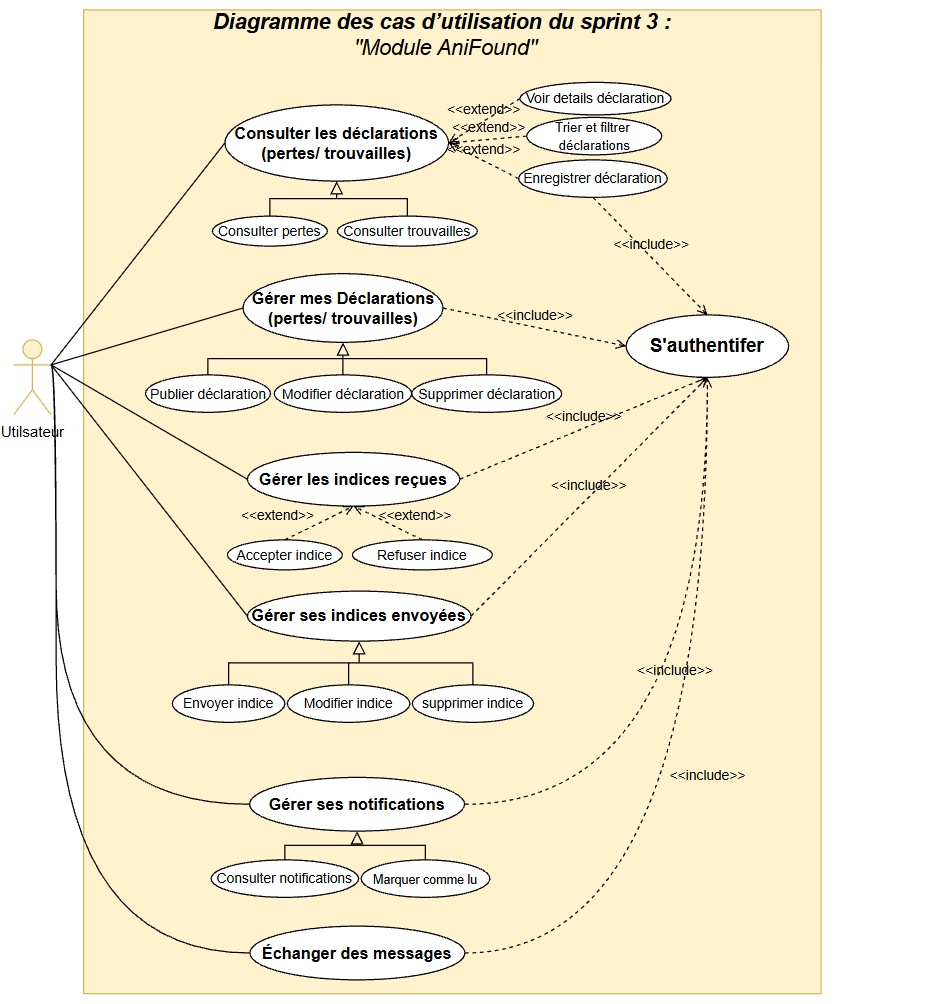
\includegraphics[width=0.92\linewidth, height=18.5cm, keepaspectratio]{images/usecase anifound.png}
    \caption{Diagramme des cas d’utilisation du sprint 3}
    \label{fig:usecase-sprint3}
\end{figure}
\newpage
\subsection{Descriptions textuelles des cas d’utilisation du sprint 3}  
Dans cette section, nous allons présenter les descriptions textuelles des cas d’utilisation du sprint 3
afin de détailler le comportement du système pour chaque fonctionnalité du module AniFound. 

\subsubsection{ Description textuelle du cas d’utilisation «Consulter déclarations de perte et de trouvaille » }    

La table \ref{tab:consulter_declarations} présente la description textuelle du cas d’utilisation « Consulter les déclarations de perte et de trouvaille » : 

\begin{longtable}{|c|p{11cm}|}
\caption{Description textuelle du cas d’utilisation "Consulter les déclarations de perte et de trouvaille"}
\label{tab:consulter_declarations} \\
\hline
\cellcolor{coloranifound} \textbf{Nom du cas d'utilisation } & Consulter les déclarations de perte et de trouvaille \\
\hline
\cellcolor{coloranifound} \textbf{Acteurs} & Utilisateur \\
\hline
\cellcolor{coloranifound} \textbf{Description } & Tout utilisateur peut consulter les annonces de perte et de trouvaille du module AniFound pour identifier un animal perdu ou retrouvé. \\
\hline
\cellcolor{coloranifound} \textbf{Pré-condition } & L’utilisateur doit avoir accès à la plateforme AniHub. \\
\hline
\cellcolor{coloranifound} \textbf{Post-condition } & L’utilisateur a consulté et éventuellement enregistré des déclarations pour un suivi ultérieur. \\
\hline
\cellcolor{coloranifound} \textbf{Scénario nominal } & 
\begin{enumerate}
\item L’utilisateur accède au module AniFound.
\item Le système redirige l’utilisateur vers le module AniFound.
\item L’utilisateur choisit la section « déclarations de perte » ou « déclarations de trouvaille ».
\item Le système affiche la liste des déclarations correspondantes.
\item L’utilisateur peut filtrer les déclarations selon différents critères (type, localisation, date).
\item L’utilisateur peut trier les déclarations par date (plus récentes ou plus anciennes).
\item Le système affiche les résultats filtrés et triés.
\item L’utilisateur peut sélectionner une déclaration pour consulter ses détails.
\item L’utilisateur peut enregistrer une déclaration dans sa liste d'enregistrements.
\item Le système ajoute la déclaration à la liste enregistrée de l’utilisateur.
\end{enumerate} \\
\hline
\end{longtable}
\newpage 
\subsubsection{Description textuelle du cas d’utilisation «Gérer déclarations de perte et de trouvaille»}
La table \ref{tab:gerer_declarations} présente la description textuelle du cas d’utilisation « Gérer les déclarations de perte et de trouvaille » :
\begin{longtable}{|c|p{11cm}|}
\caption{Description textuelle du cas d'utilisation "Gérer les déclarations de perte et de trouvaille"}
\label{tab:gerer_declarations} \\
\hline
\cellcolor{coloranifound}\textbf{Nom du cas d'utilisation } & Gérer les déclarations de perte et de trouvaille \\
\hline
\cellcolor{coloranifound}\textbf{Acteurs} & Utilisateur \\
\hline
\cellcolor{coloranifound}\textbf{Description } & L’utilisateur peut publier, modifier ou supprimer une déclaration de perte ou de trouvaille \\
\hline
\cellcolor{coloranifound}\textbf{Pré-condition } & L’utilisateur doit être authentifié \\
\hline
\cellcolor{coloranifound}\textbf{Post-condition } & La déclaration est ajoutée, modifiée ou supprimée avec succès. \\
\hline

\cellcolor{coloranifound}\textbf{Scénario nominal } &
\begin{enumerate}
\item L’utilisateur accède au module AniFound.
\item Le système redirige l’utilisateur vers "AniFound".

\item \textbf{Cas publication :}
\begin{itemize}
\item L’utilisateur choisit « perte » ou « trouvaille ».
\item L’utilisateur clique sur « Publier une déclaration ».
\item Le système affiche le formulaire d’ajout.
\item L’utilisateur remplit les informations et valide.
\item Le système vérifie et enregistre la déclaration.
\end{itemize}

\item L’utilisateur accède à « Mon espace AniFound ».
\item Le système affiche ses déclarations.

\item \textbf{Cas modification :}
\begin{itemize}
\item L’utilisateur sélectionne une déclaration.
\item L’utilisateur clique sur « Modifier ».
\item Le système affiche le formulaire pré-rempli.
\item L’utilisateur modifie et valide.
\item Le système enregistre les modifications.
\end{itemize}

\item \textbf{Cas suppression :}
\begin{itemize}
\item L’utilisateur sélectionne une déclaration.
\item L’utilisateur clique sur « Supprimer ».
\item Le système demande une confirmation.
\item L’utilisateur confirme.
\item Le système supprime la déclaration.
\end{itemize}

\item Le système affiche un message de succès.
\end{enumerate} \\

\hline
\cellcolor{coloranifound}\textbf{Scénario alternatif :} &
\begin{itemize}
\item Erreur de publication : message d’erreur affiché.
\item Erreur de modification : message d’erreur affiché.
\item Annulation suppression : Déclaration conservée.
\end{itemize} \\
\hline

\end{longtable}
\newpage 
\subsubsection{ Description textuelle des cas d’utilisation «Gérer les indices reçus et envoyés» }   
La table \ref{tab:gerer_indices_anifound} présente la description textuelle du cas d’utilisation «Gérer les indices reçus et envoyés» :
\begin{longtable}{|c|p{11cm}|} 
\caption{Description textuelle des cas d'utilisation "Gérer les indices reçus et envoyés"}
\label{tab:gerer_indices_anifound} \\
\hline
\cellcolor{coloranifound}\textbf{Nom du cas d'utilisation } & Gérer les indices reçus et envoyés \\
\hline
\cellcolor{coloranifound}\textbf{Acteurs} & Utilisateur \\
\hline
\cellcolor{coloranifound}\textbf{Description } & L’utilisateur consulte et gère les indices de ses déclarations de trouvaille pour prouver la propriété d’un animal. \\
\hline
\cellcolor{coloranifound}\textbf{Pré-condition } & L’utilisateur est authentifié et dispose de déclarations de trouvaille ou a déjà envoyé des indices. \\
\hline
\cellcolor{coloranifound}\textbf{Post-condition } & Les indices sont consultés et leur statut est mis à jour (en attente, validé ou rejeté). \\
\hline

\cellcolor{coloranifound}\textbf{Scénario nominal } &
\begin{enumerate}
\item L’utilisateur accède au module AniFound.
\item Il sélectionne « Mon espace AniFound ».
\item Le système affiche les déclarations de l’utilisateur.
\item L’utilisateur choisit une déclaration spécifique.
\item Le système affiche les indices liés à cette déclaration.
\item Selon le type d’interaction :

\begin{itemize}
\item \textbf{Cas 1 : Indices reçus}
\begin{enumerate}
\item L’utilisateur consulte la liste des indices reçus.
\item Il ouvre un indice reçu .
\item Il valide ou rejette l’indice .
\item Le système met à jour le statut de l’indice.
\item Le système affiche un message de confirmation.
\end{enumerate}

\item \textbf{Cas 2 : Indices envoyés}
\begin{enumerate}
\item L’utilisateur consulte la liste des indices qu’il a envoyés.
\item Il sélectionne un indice pour en voir les détails.
\item Il consulte son statut (en attente, validé ou rejeté).
\item Le système affiche les mises à jour du statut.
\end{enumerate}
\end{itemize}

\end{enumerate} \\
\hline

\cellcolor{coloranifound}\textbf{Scénario alternatif :} &
\begin{itemize}
\item Erreur lors du chargement ou du traitement : le système affiche un message d’erreur sans modifier les données.
\end{itemize} \\
\hline

\end{longtable}

\newpage

\subsection{Diagramme de classes du sprint 3} 
Dans cette section, nous présentons le diagramme de classes du sprint 3, qui regroupe l’ensemble des classes constituant le système. 


La figure \ref{fig:class_diagram_anifound} illustre le diagramme de classes pour ce sprint :



\begin{figure}[H]
    \centering
    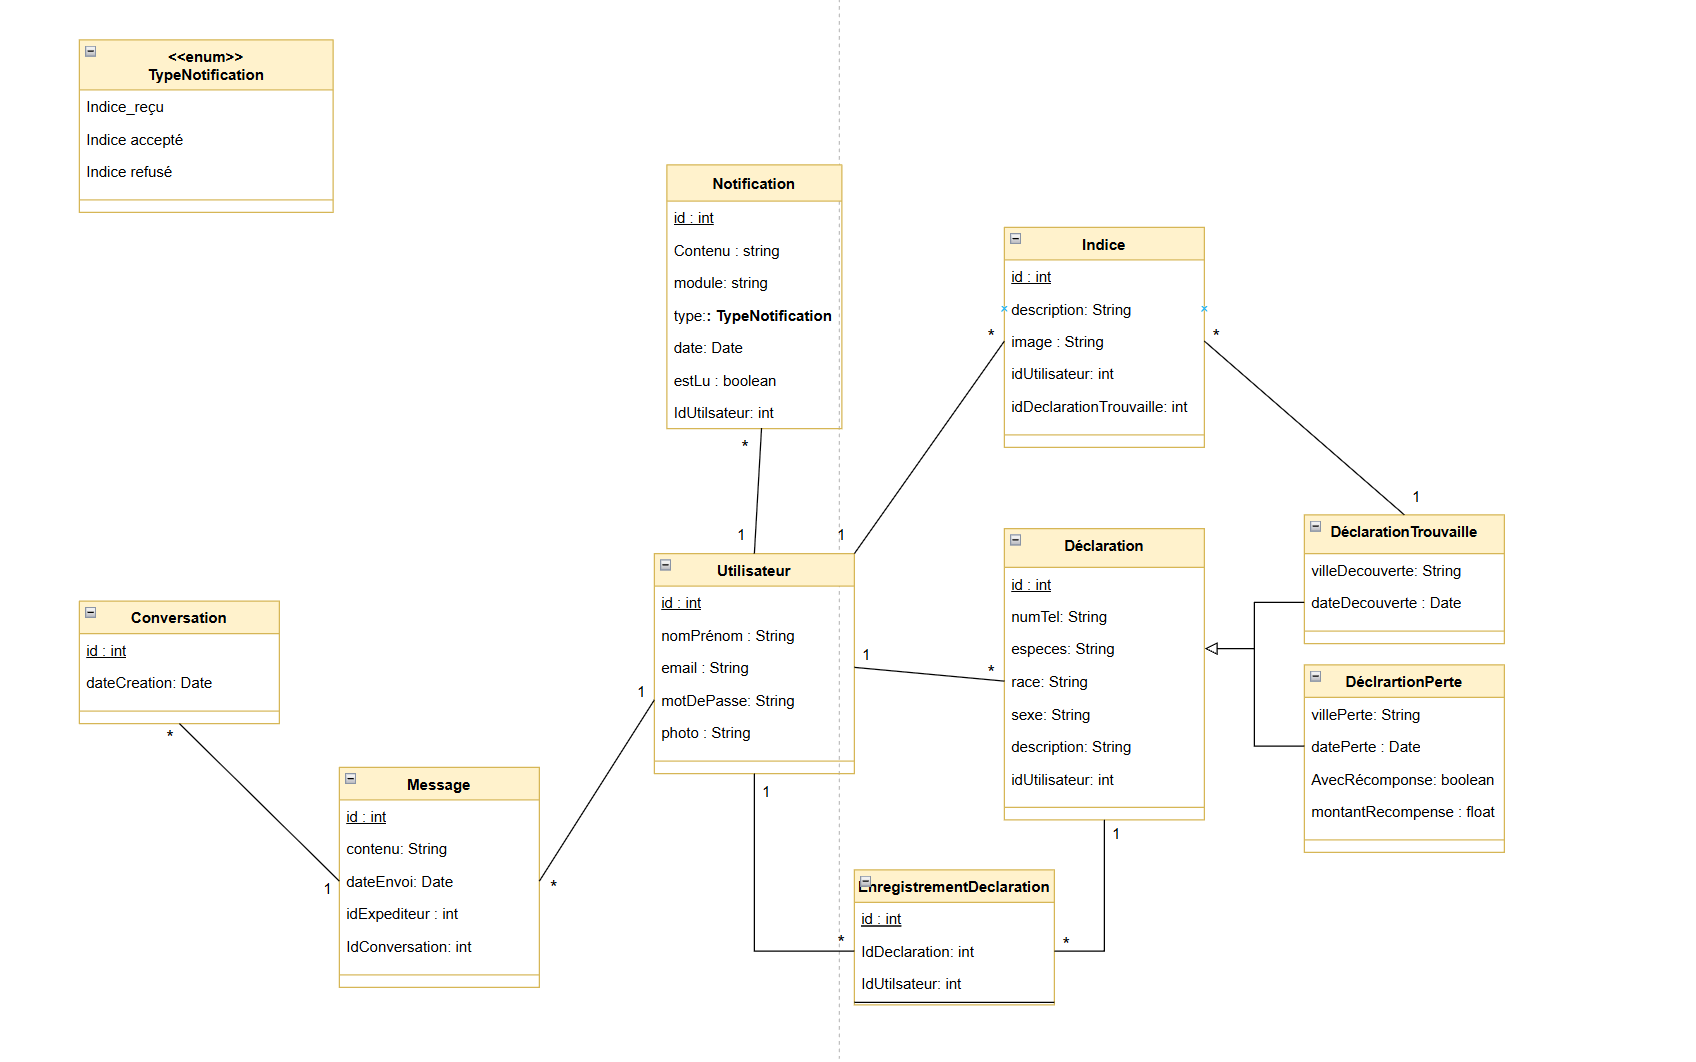
\includegraphics[width=1.15\textwidth,height=16cm]{images/diagramme classe anifoundd.png}
    \caption{Diagramme de classes du sprint 3}
    \label{fig:class_diagram_anifound}
\end{figure}

\subsection{Diagrammes de séquences du sprint 3}

Dans cette section, nous présentons les diagrammes de séquence du sprint 3, illustrant les principales interactions entre les différents composants du système et les flux de communication associés aux nouvelles fonctionnalités implémentées . 
\newpage
\subsubsection{Diagramme de séquence : gérer mes déclarations de perte ou de trouvaille}

La figure \ref{fig:gerer_declarations_sq} illustre les interactions entre l’utilisateur et le système pour la gestion des déclarations de perte ou de trouvaille.

\begin{figure}[H]
    \centering
    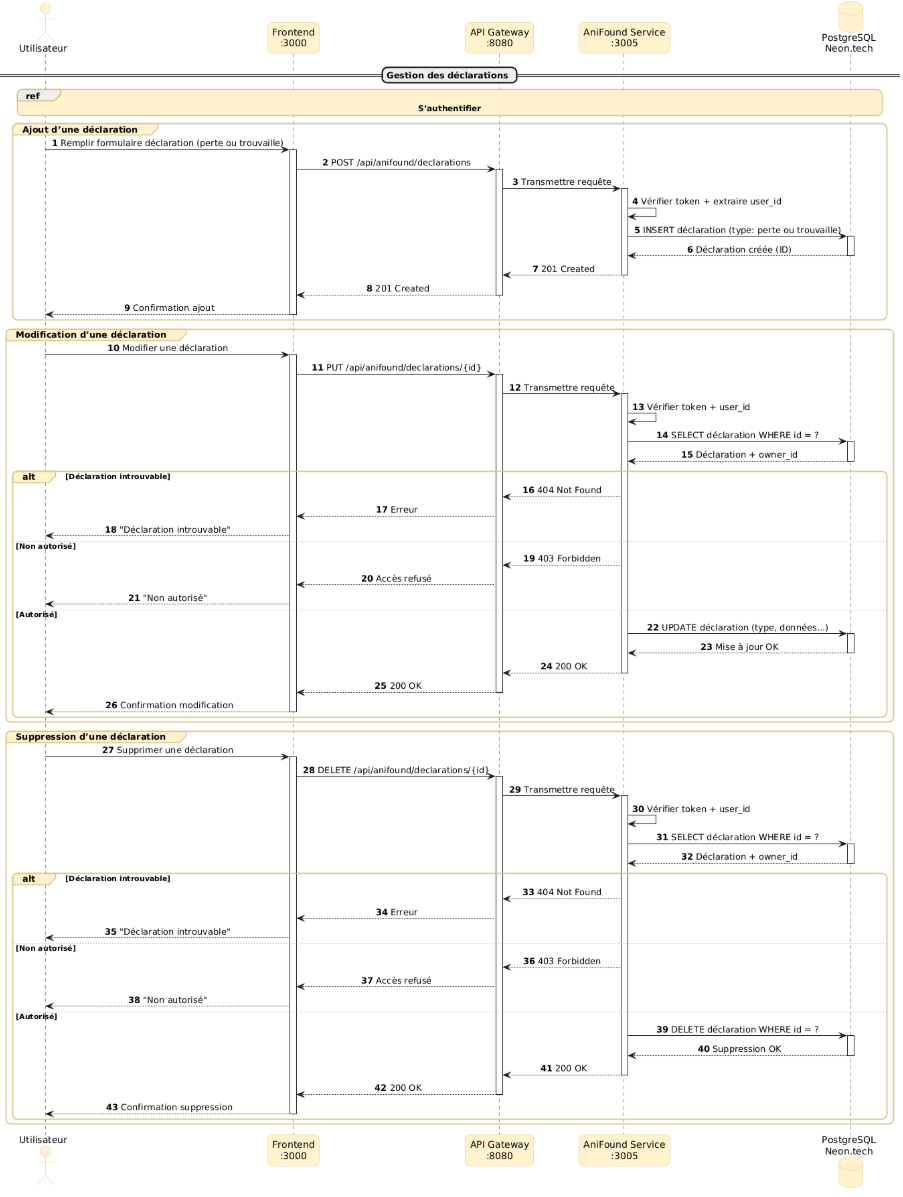
\includegraphics[width=0.7\textwidth]{images/gerer declarations sq.png}
    \caption{Diagramme de séquence : gérer mes déclarations de perte ou de trouvaille}
    \label{fig:gerer_declarations_sq}
\end{figure}
\newpage  
\subsubsection{Diagramme de séquence : gérer mes indices reçus}

La figure \ref{fig:gerer_indices_recus_sq} illustre les différentes interactions entre l’utilisateur et le système lors de la gestion des indices reçus liés aux déclarations de perte ou de trouvaille. Elle montre le processus de consultation des indices, ainsi que les actions possibles de validation ou d’ignorance d’un indice. Les échanges entre le Frontend, l’API Gateway, le microservice AniFound, la base de données et le service de notification sont également présentés afin de mettre en évidence le traitement complet d’un indice reçu : 
\begin{figure}[H]
    \centering
    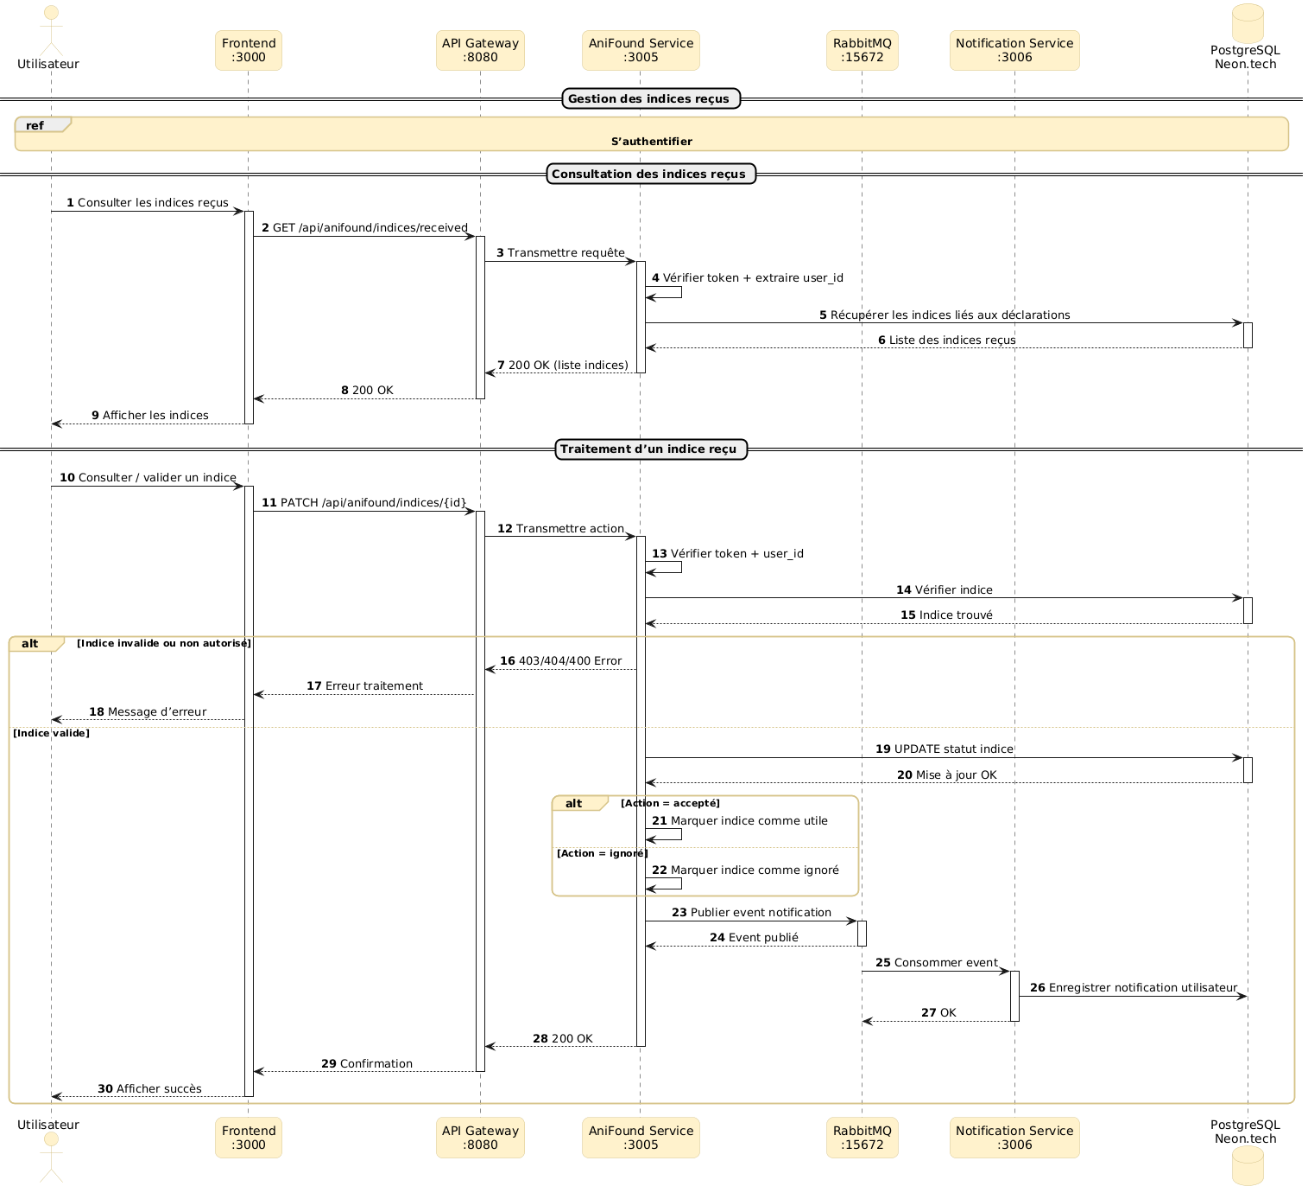
\includegraphics[width=1\textwidth]{images/gerer indice recu sq.png}
    \caption{Diagramme de séquence : gérer mes indices reçus}
\end{figure}
\newpage
\subsection{Réalisation du sprint 3 }

Dans cette partie, nous présentons les différentes interfaces graphiques de l’application développée, en lien avec ce sprint :

\subsubsection{Menu principal de l’application AniHub et interface d’accueil AniFound} 

La figure \ref{fig:menu_anifound_accueil} illustre le menu principal de l’application AniHub ainsi que l’interface d’accueil du module AniFound.

\begin{figure}[h!]
    \centering
    
    \begin{minipage}{0.48\textwidth}
        \centering
        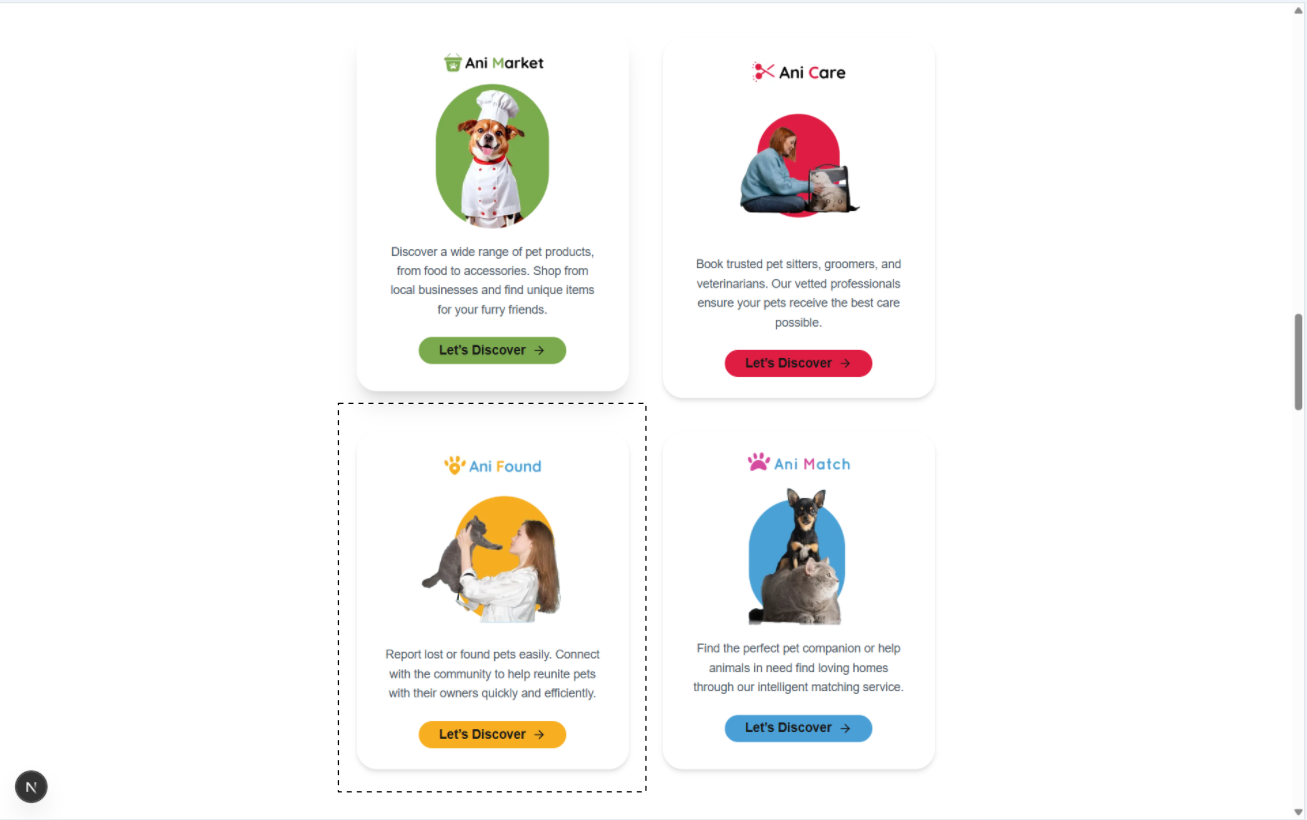
\includegraphics[width=0.85\textwidth]{images/menu anifound.png}
        \caption{Menu principal de l’application AniHub}
        \label{fig:menu_anihub_anifound}
    \end{minipage}
    \hfill
    \begin{minipage}{0.48\textwidth}
        \centering
        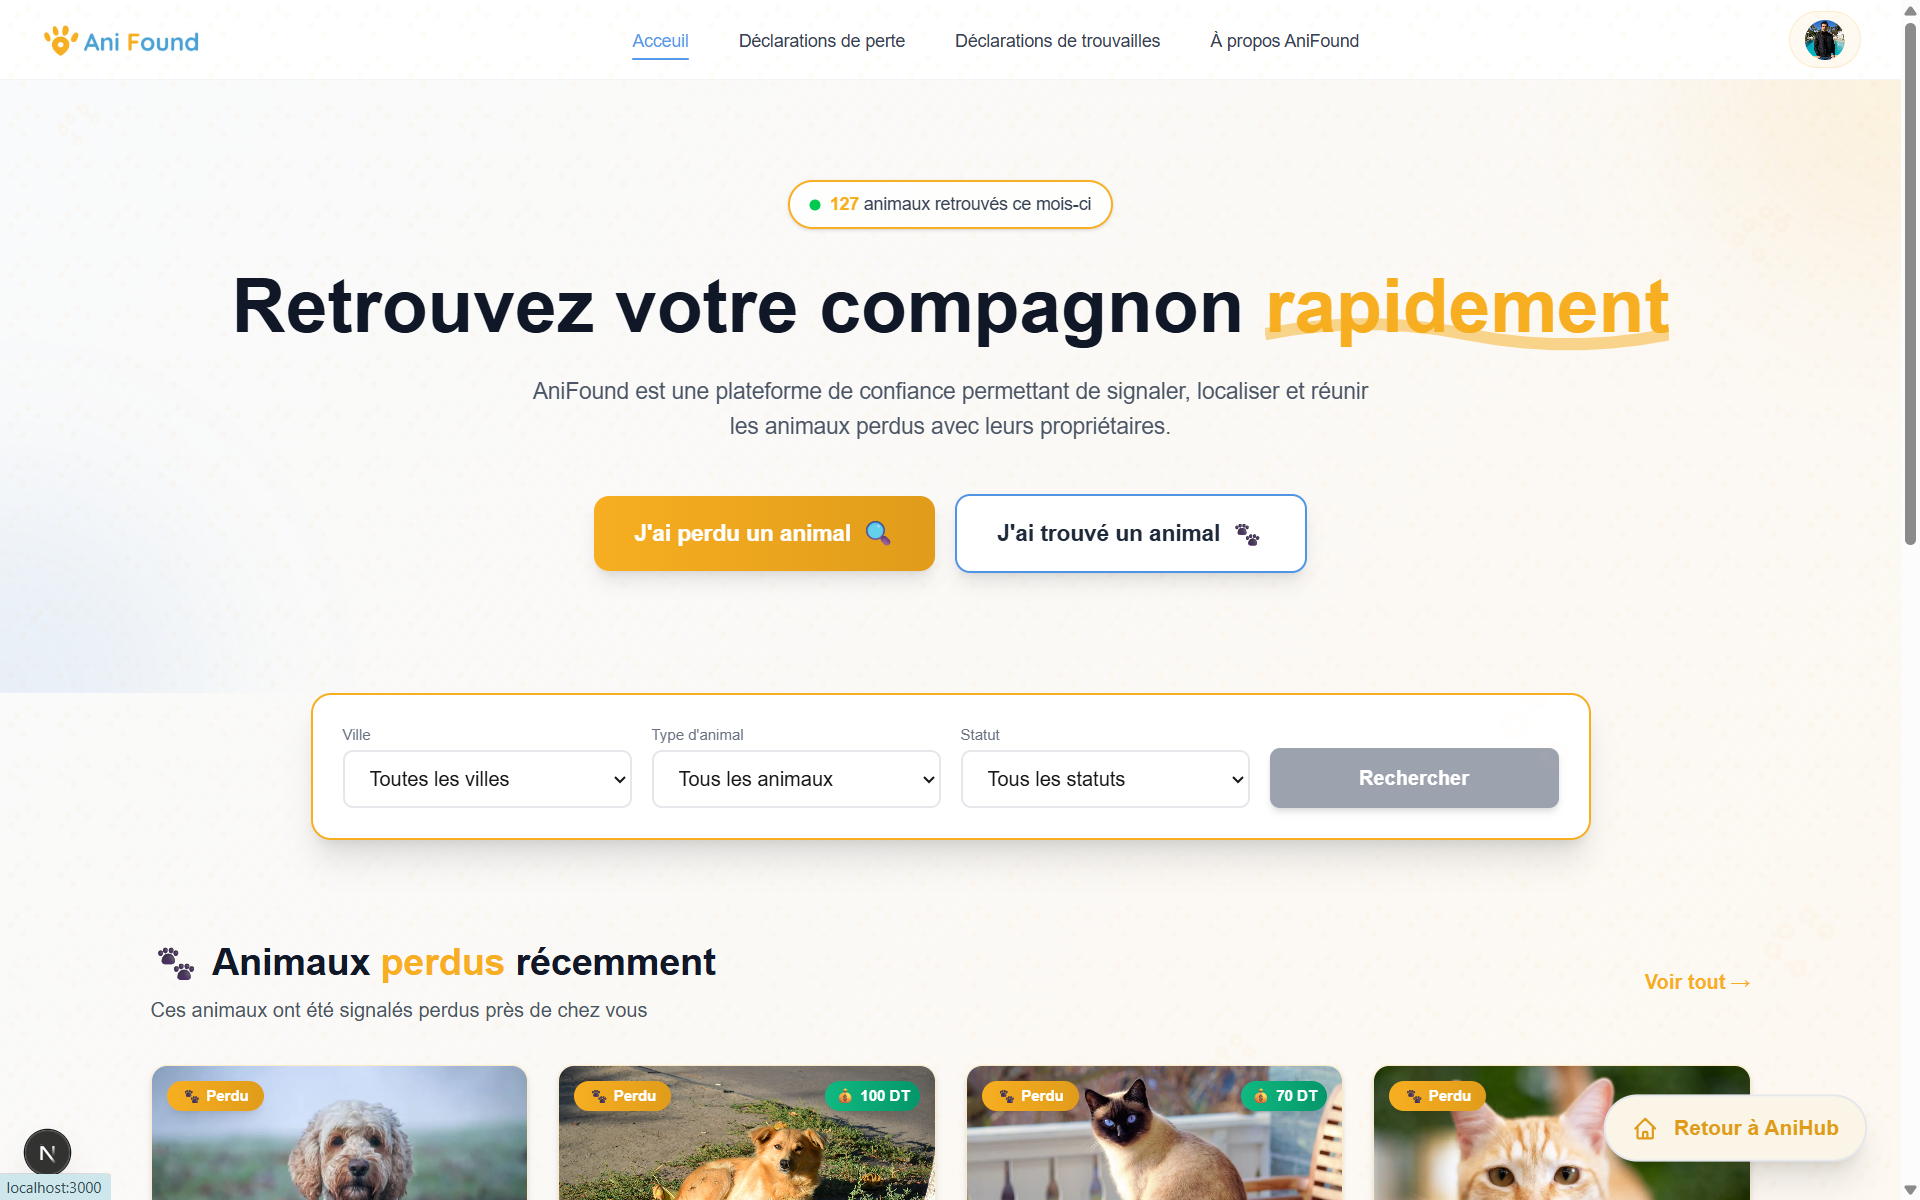
\includegraphics[width=0.85\textwidth]{images/acceuil anifound.png}
        \caption{Interface d’accueil AniFound}
        \label{fig:acceuil_anifound}
    \end{minipage}

\end{figure}  

\subsubsection{Interfaces d’annonce de perte et de trouvaille}

La figure \ref{fig:annonces_perte_trouvaille} illustre les interfaces de création d’une annonce de perte et de trouvaille.

\begin{figure}[h!]
    \centering
    
    \begin{minipage}{0.48\textwidth}
        \centering
        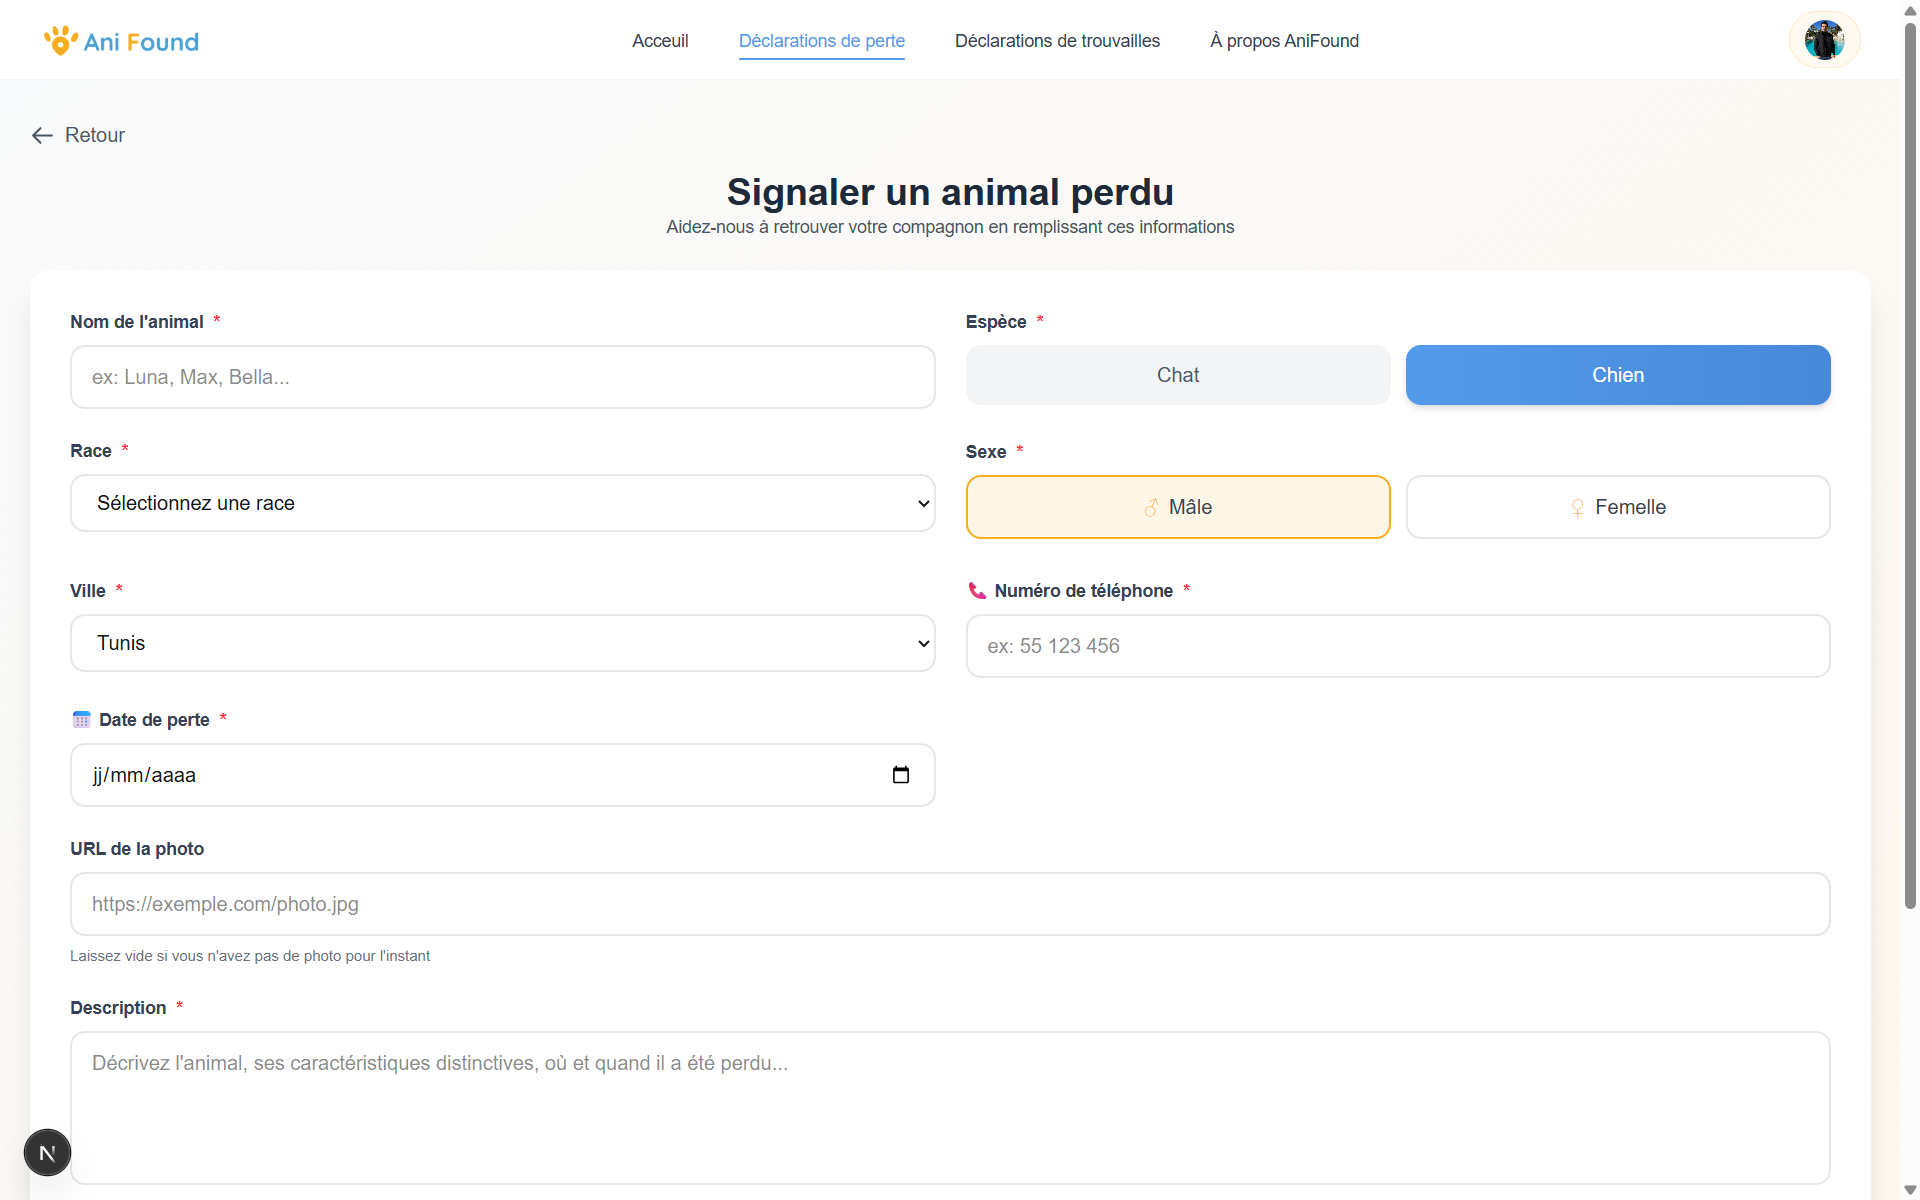
\includegraphics[width=0.77\textwidth]{images/declarer perte .png}
        \caption{Interface d’annonce de perte d’un animal}
        \label{fig:annonce_perte}
    \end{minipage}
    \hfill
    \begin{minipage}{0.48\textwidth}
        \centering
        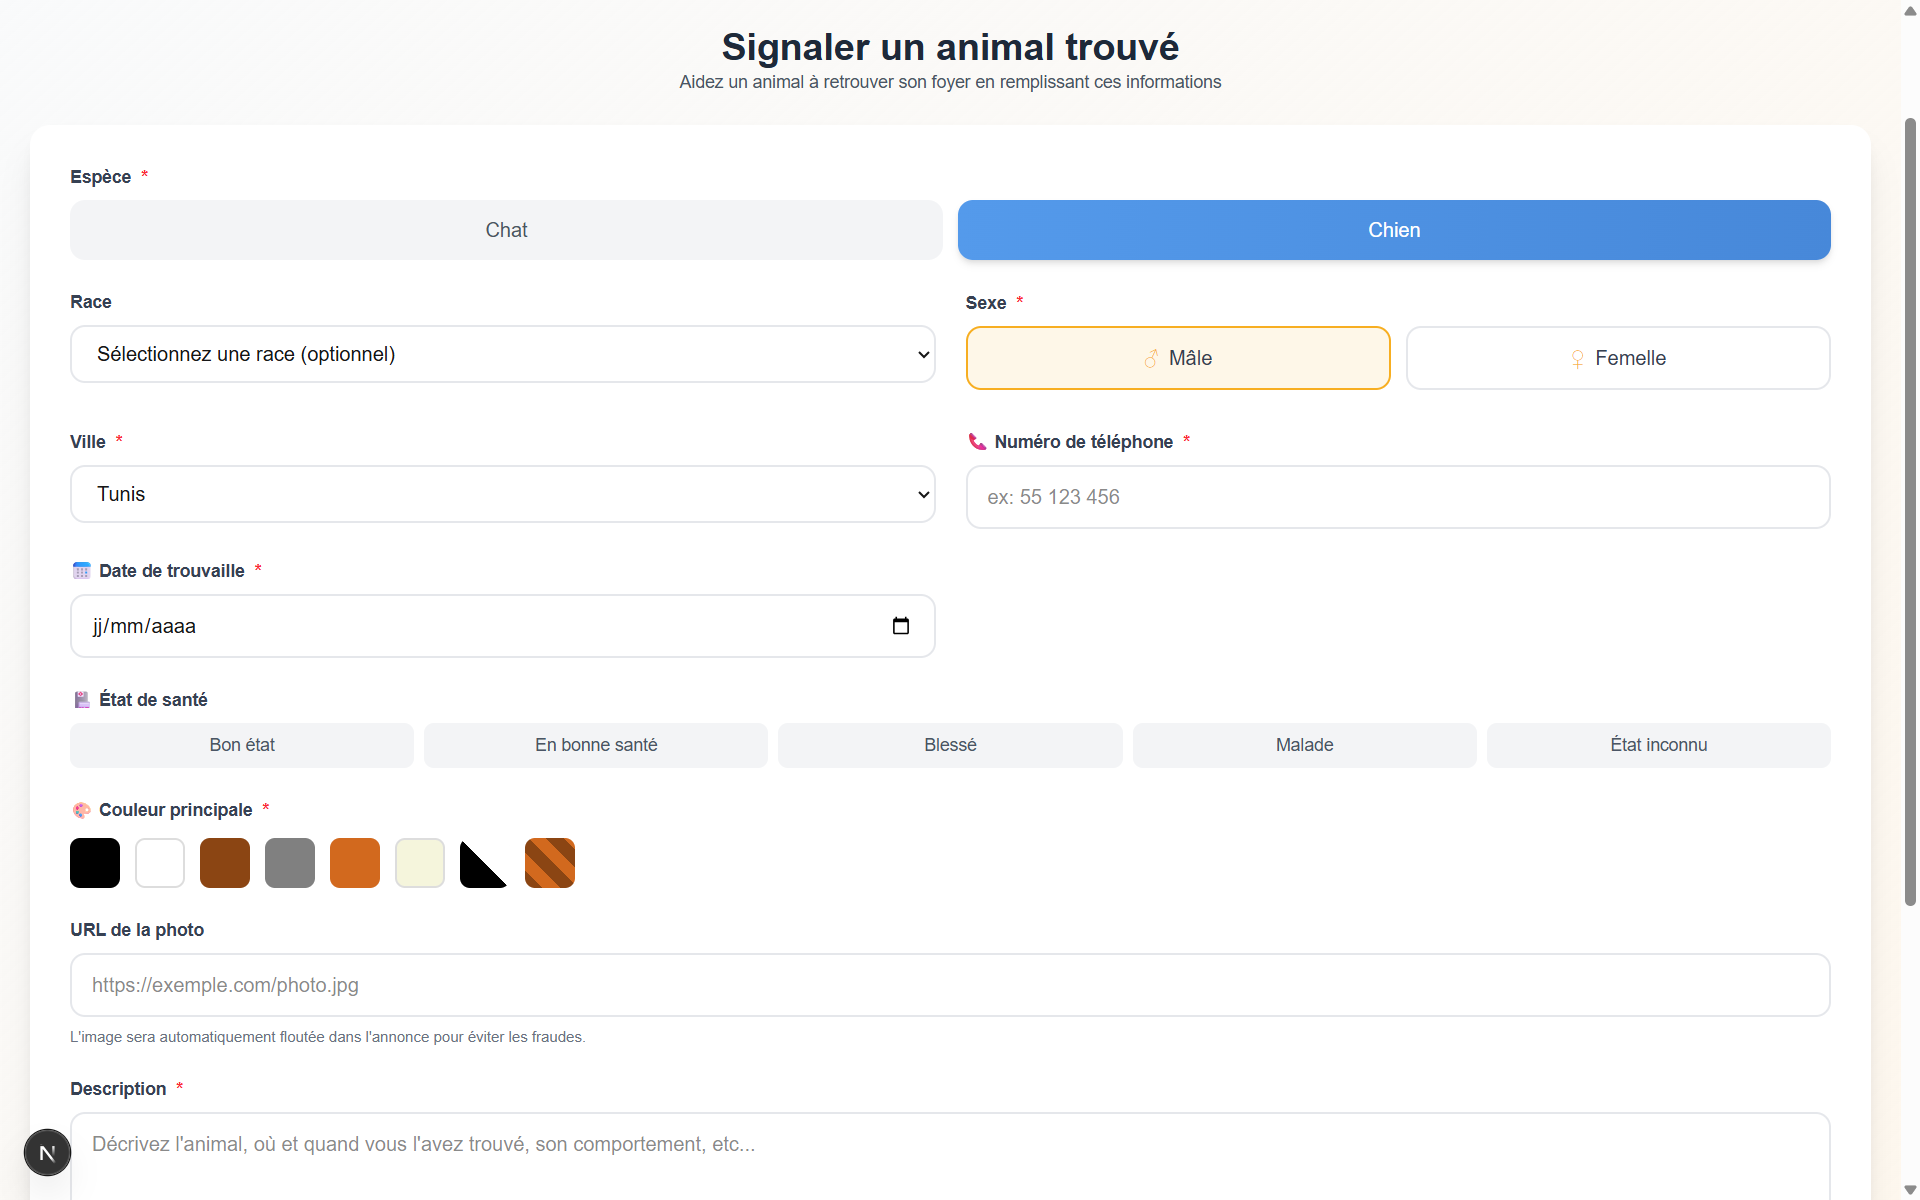
\includegraphics[width=0.77\textwidth]{images/decalarer trouvaille.png}
        \caption{Interface d’annonce de trouvaille d’un animal}
        \label{fig:annonce_trouvaille}
    \end{minipage}

\end{figure}

\newpage

\subsubsection{Interface des déclarations de trouvaille}

La figure \ref{fig:liste_trouvailles} illustre la liste des déclarations de trouvaille disponibles dans le système.

\begin{figure}[h!]
    \centering
    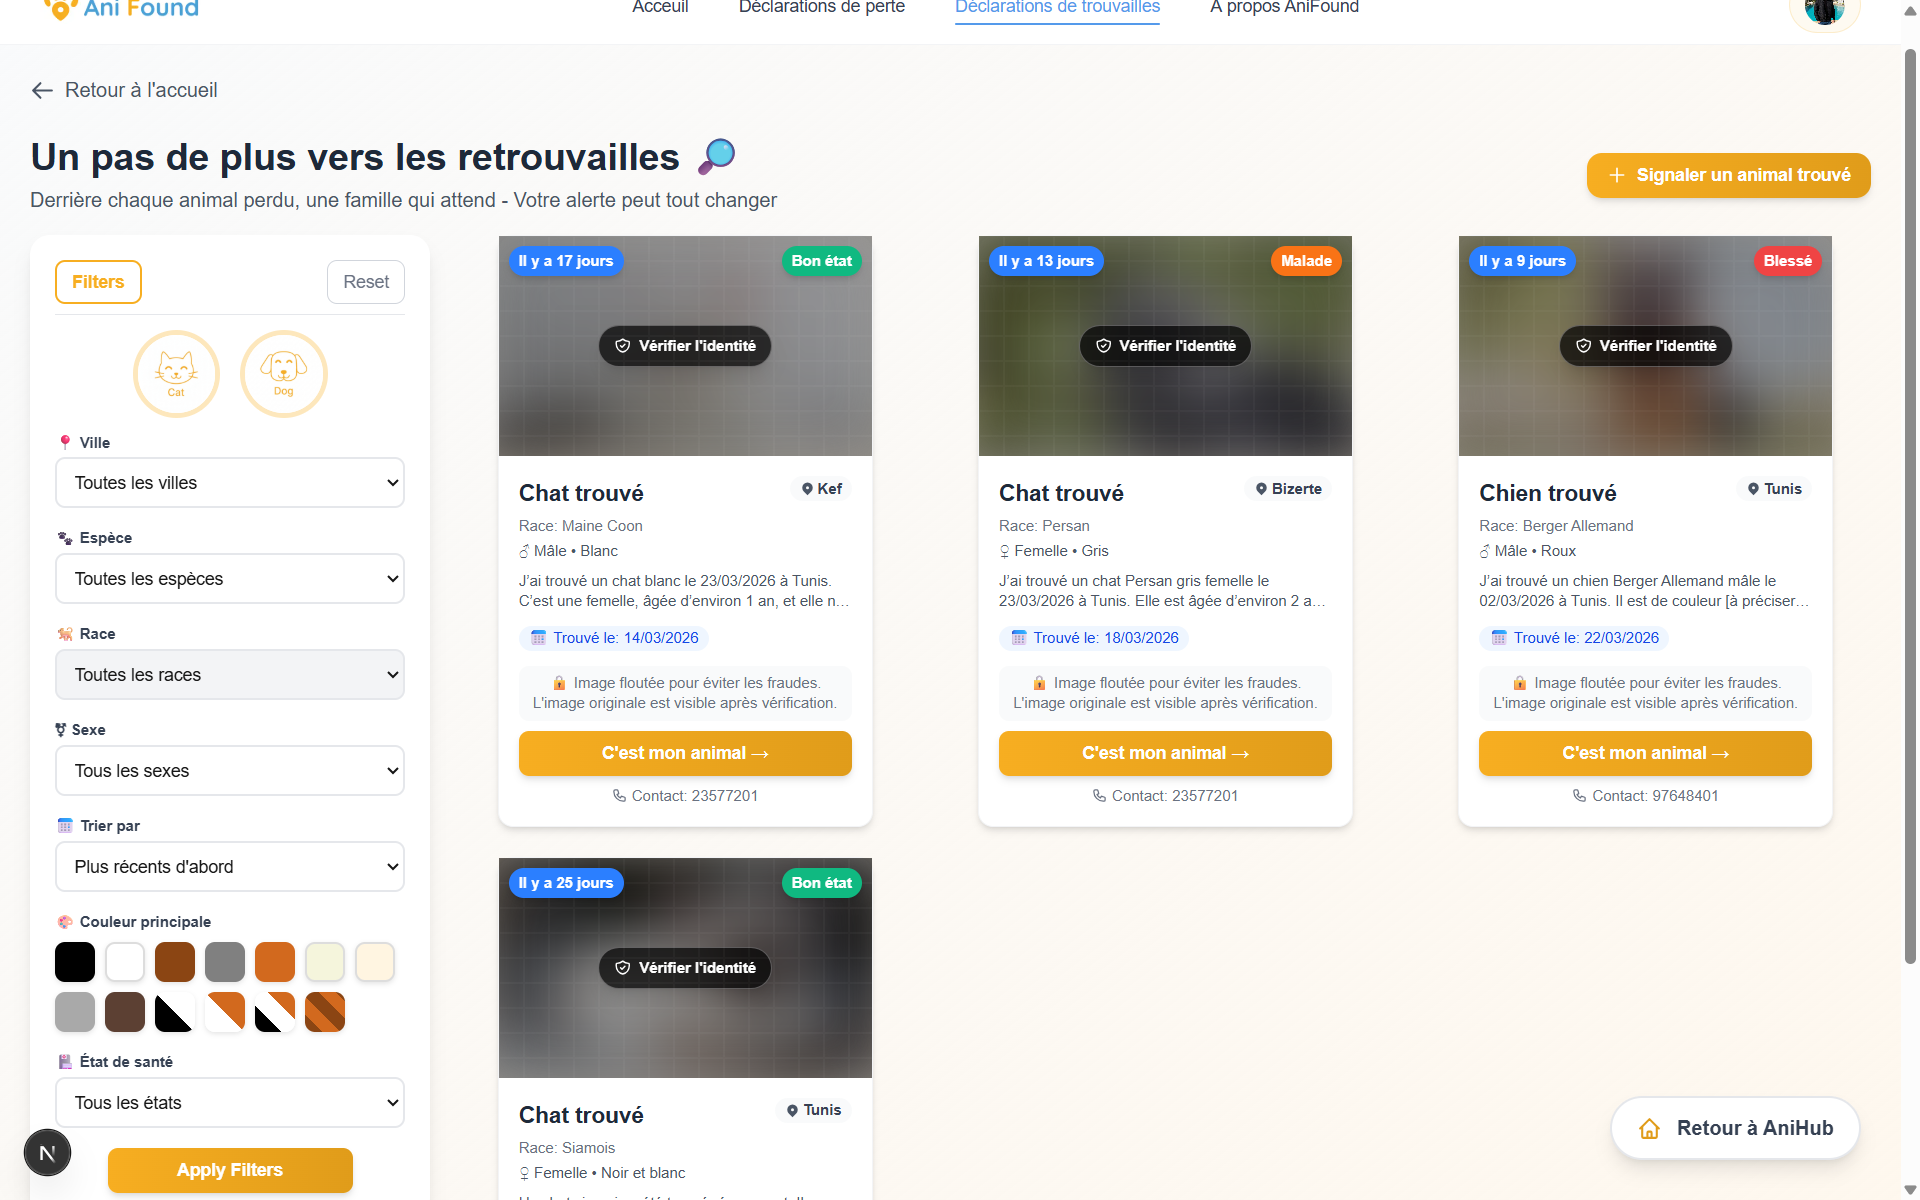
\includegraphics[width=0.77\textwidth]{images/page trouvailles.png}
    \caption{Interface des déclarations de trouvaille}
    \label{fig:liste_trouvailles}
\end{figure}  

\subsubsection{Interface de détails d’une déclaration de trouvaille}

La figure \ref{fig:details_trouvaille} illustre les détails complets d’une déclaration de trouvaille.

\begin{figure}[h!]
    \centering
    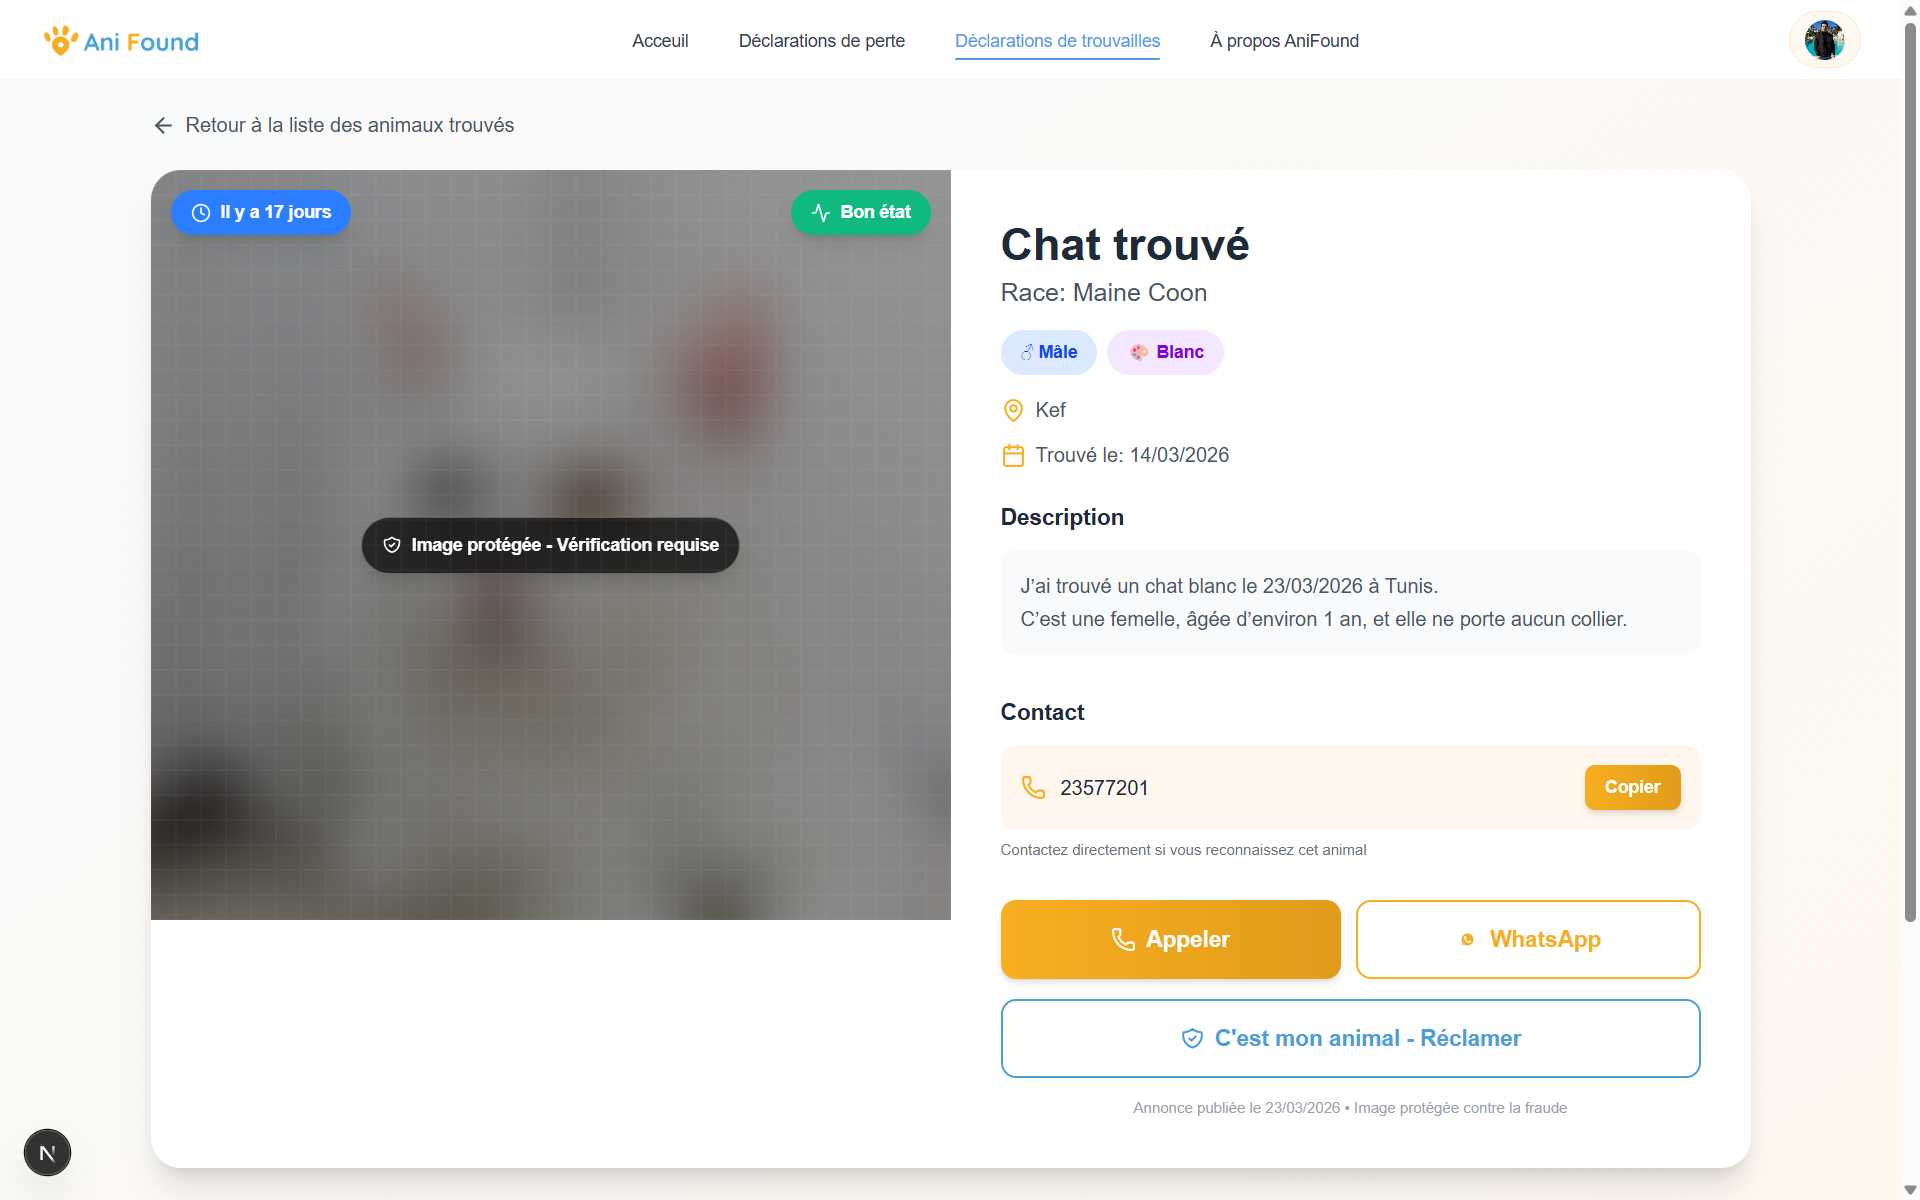
\includegraphics[width=0.77\textwidth]{images/details trouvaille.png}
    \caption{Interface de détails d’une déclaration de trouvaille}
    \label{fig:details_trouvaille}
\end{figure} 

\subsubsection{Interface d’envoi d’un indice pour une déclaration de trouvaille}

La figure \ref{fig:envoi_indice} illustre le formulaire d’envoi d’un indice pour une déclaration de trouvaille.

\begin{figure}[h!]
    \centering
    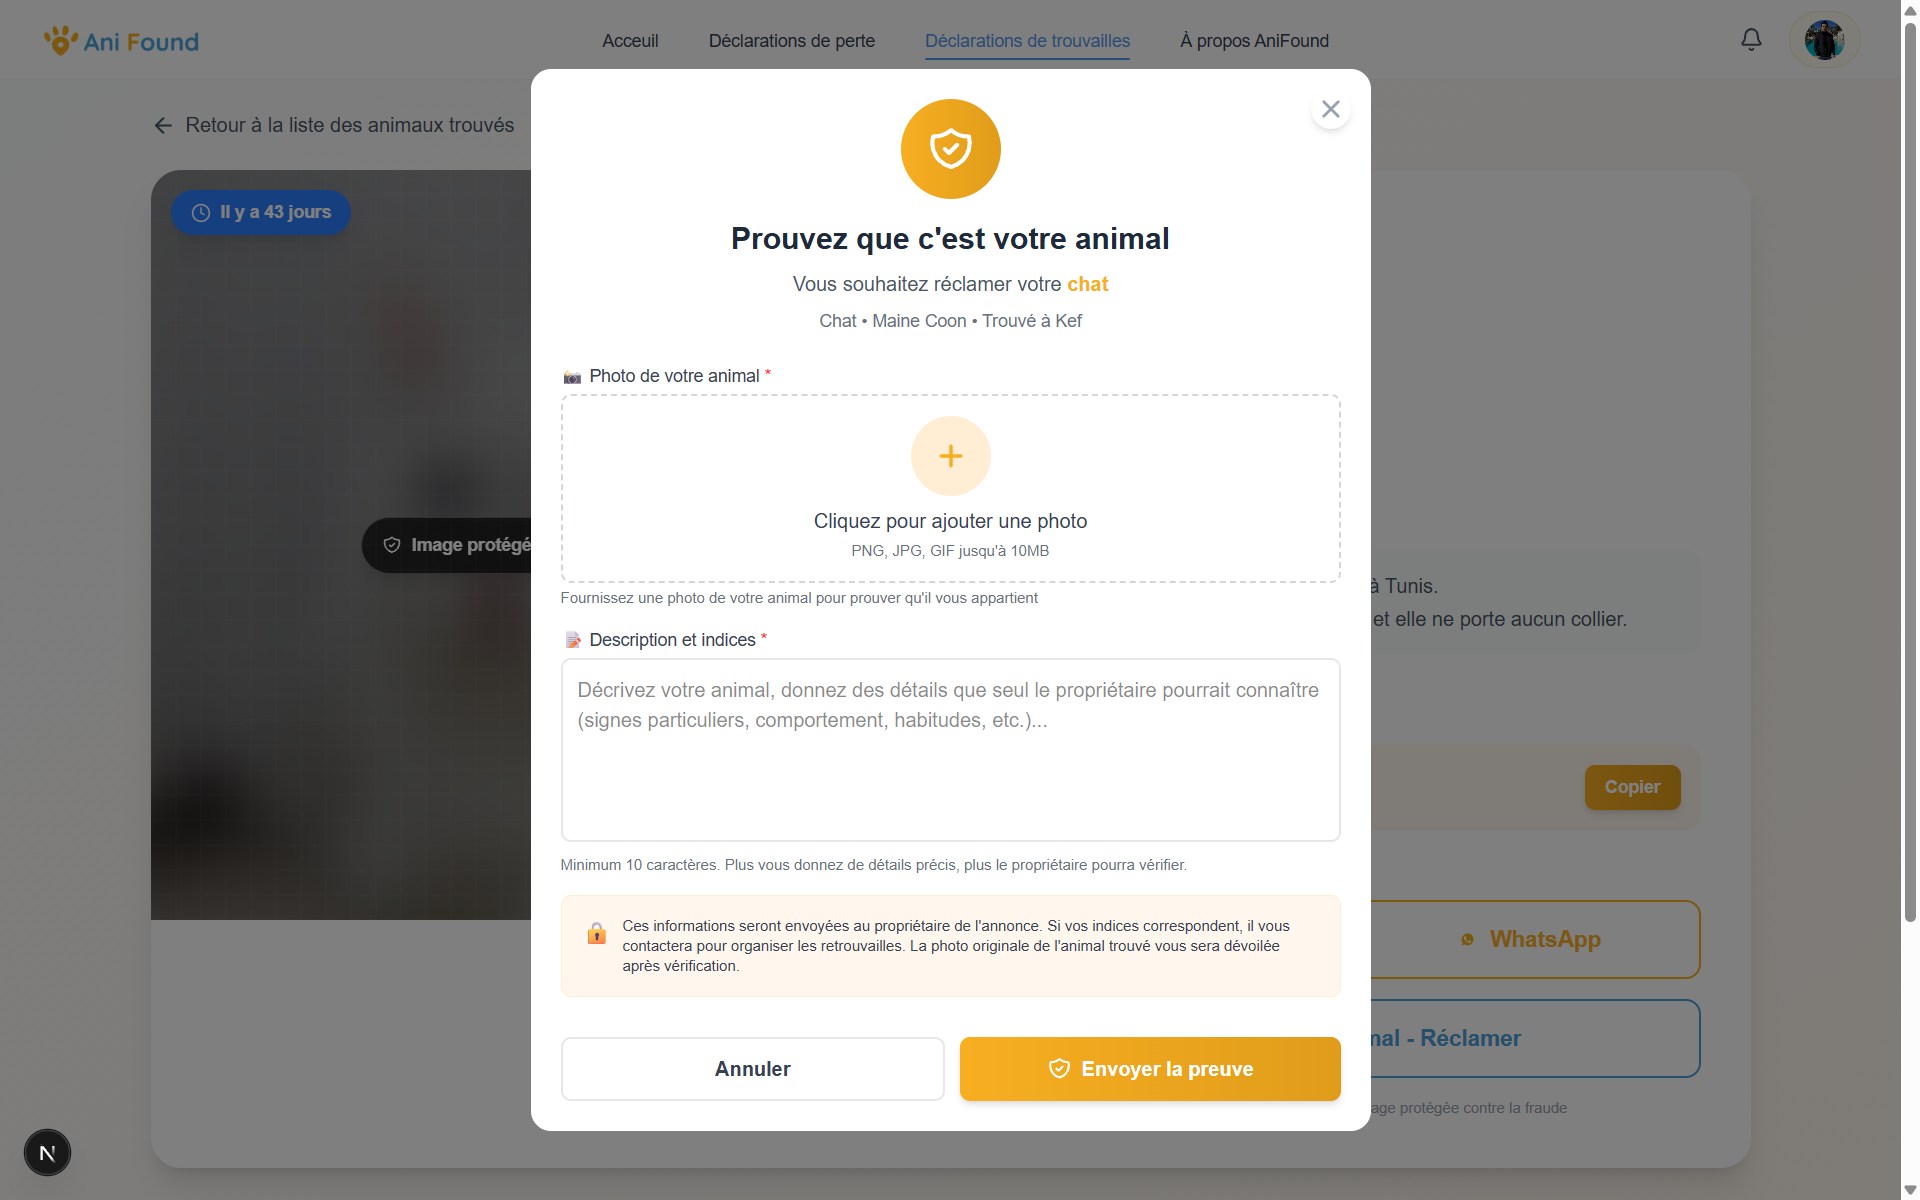
\includegraphics[width=0.77\textwidth]{images/envoyer indice.png}
    \caption{Interface d’envoi d’un indice pour une déclaration de trouvaille}
    \label{fig:envoi_indice}
\end{figure}

\subsubsection{Interface des déclarations de perte}

La figure \ref{fig:liste_pertes} illustre la liste des déclarations de perte des animaux.

\begin{figure}[h!]
    \centering
    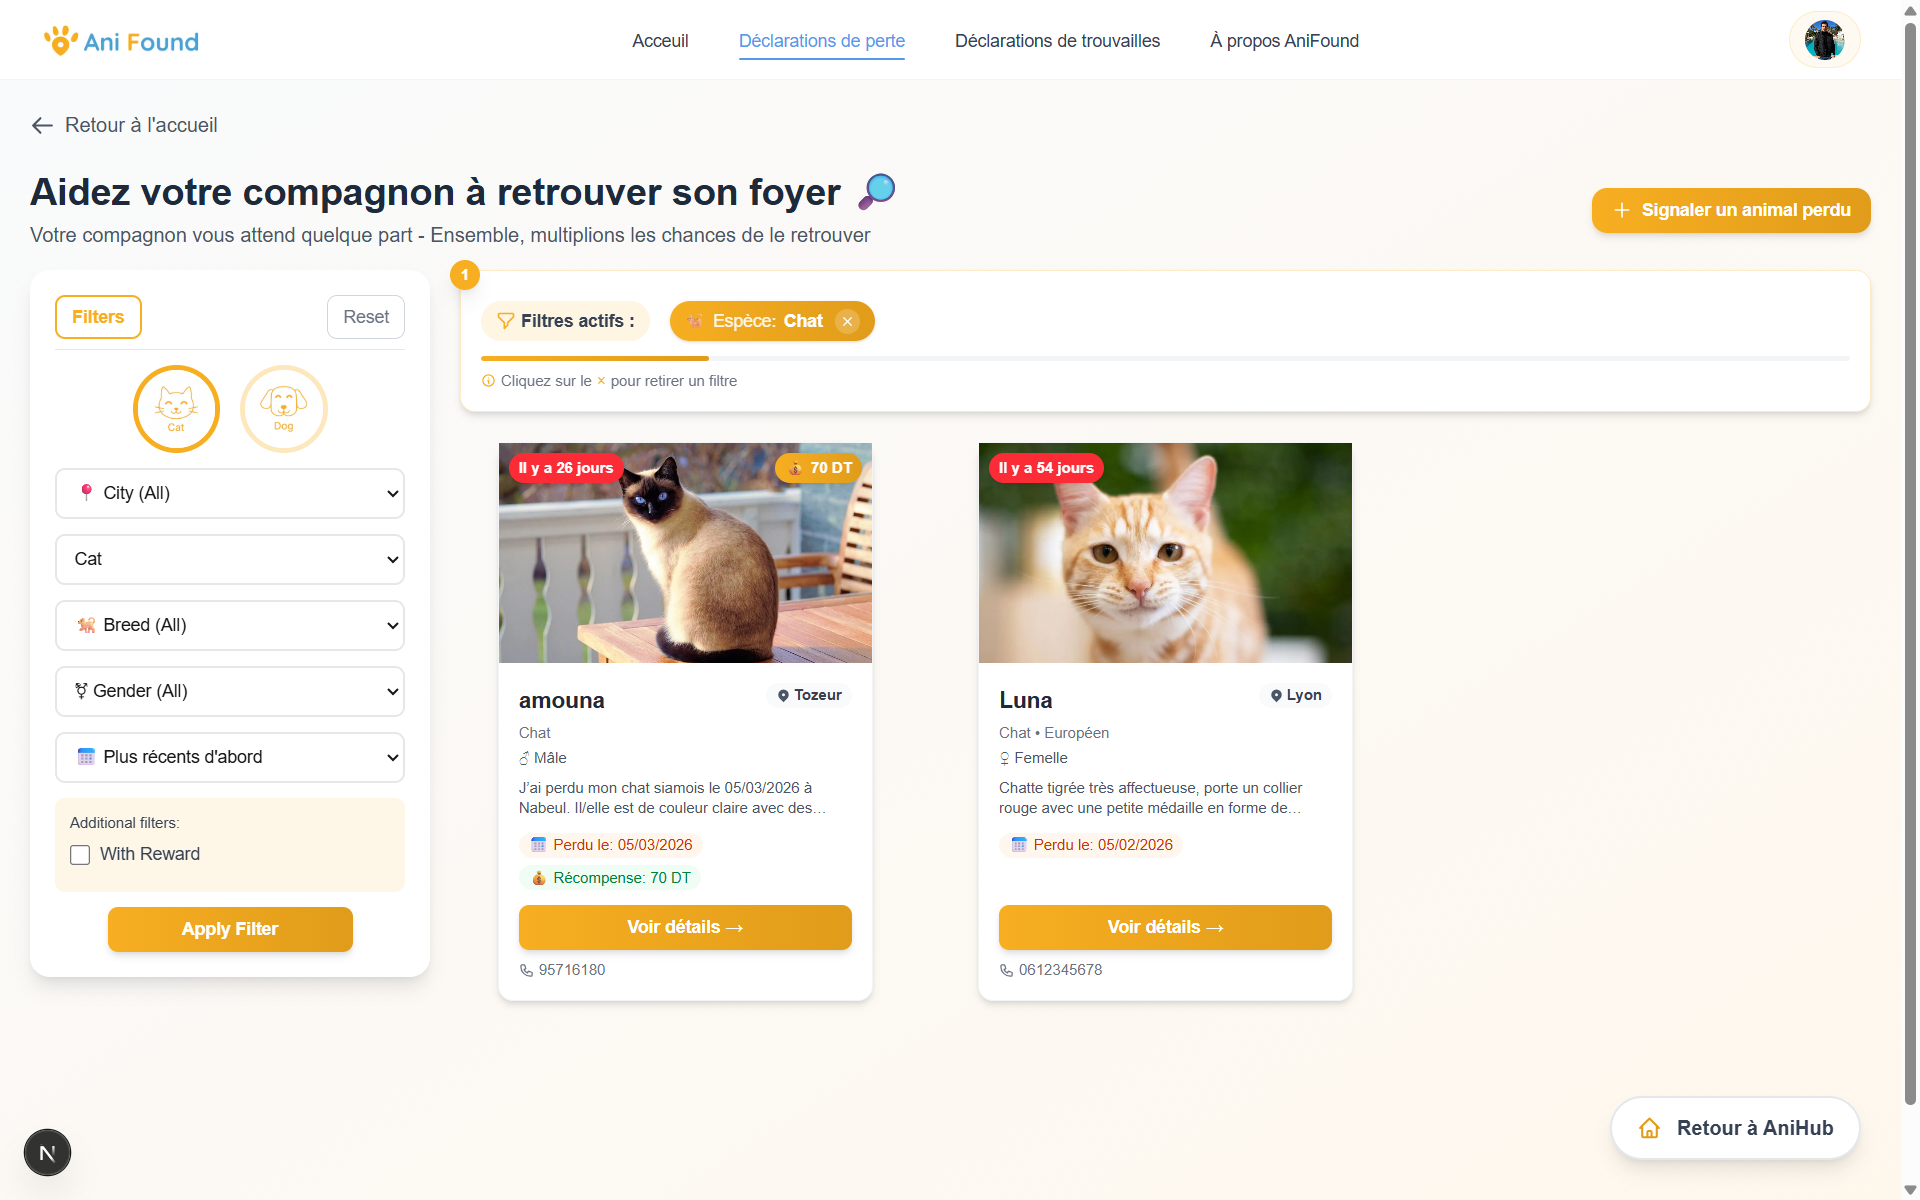
\includegraphics[width=0.77\textwidth]{images/page perte.png}
    \caption{Interface des déclarations de perte}
    \label{fig:liste_pertes}
\end{figure} 

\newpage

\subsubsection{Interface de détails d’une déclaration de perte}

La figure \ref{fig:details_perte} illustre les détails d’une déclaration de perte.

\begin{figure}[h!]
    \centering
    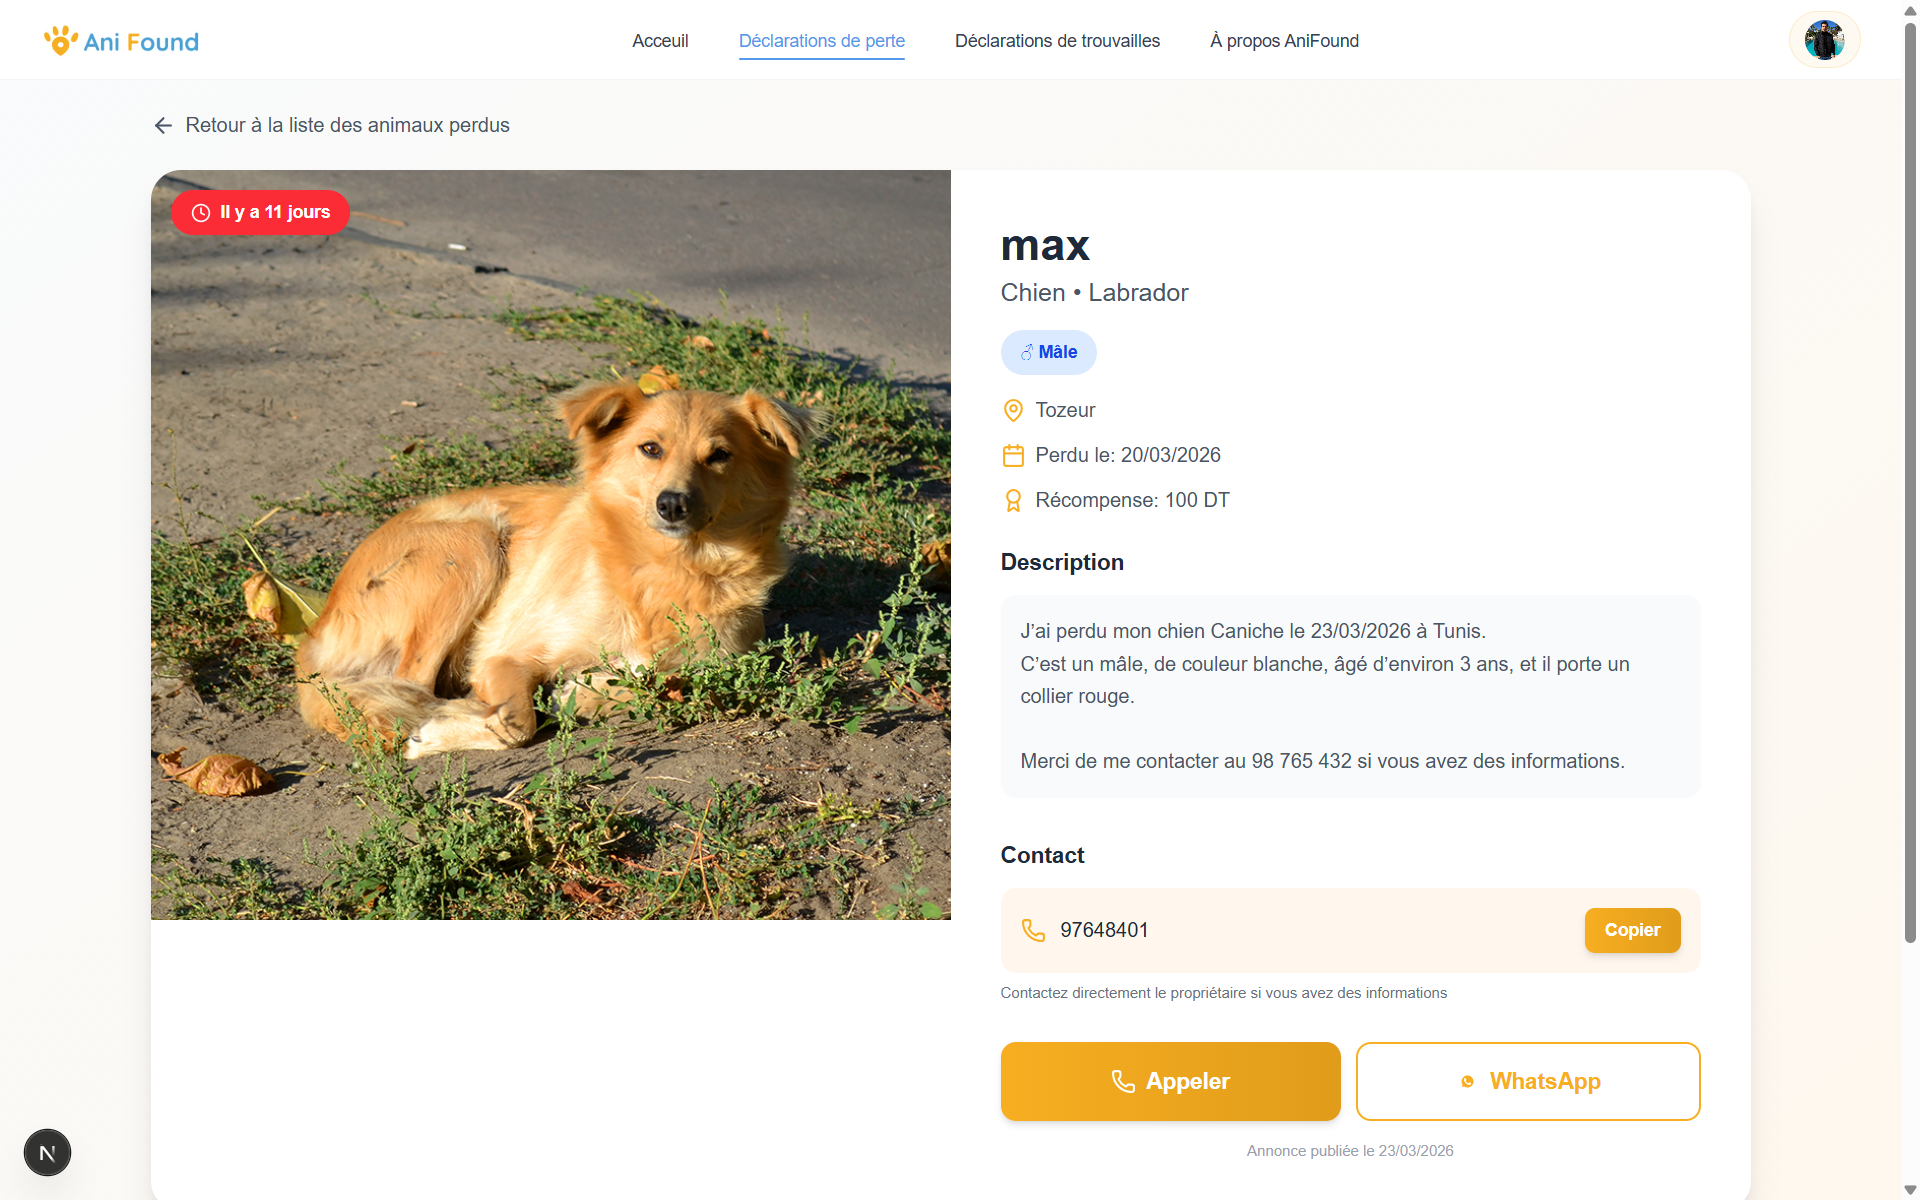
\includegraphics[width=0.77\textwidth]{images/details perte.png}
    \caption{Interface de détails d’une déclaration de perte}
    \label{fig:details_perte}
\end{figure}  

\subsubsection{Interface de l’espace AniFound et gestion du profil}

La figure \ref{fig:espace_anifound_profil} illustre l’espace utilisateur AniFound ainsi que la gestion du profil.

\begin{figure}[h!]
    \centering
    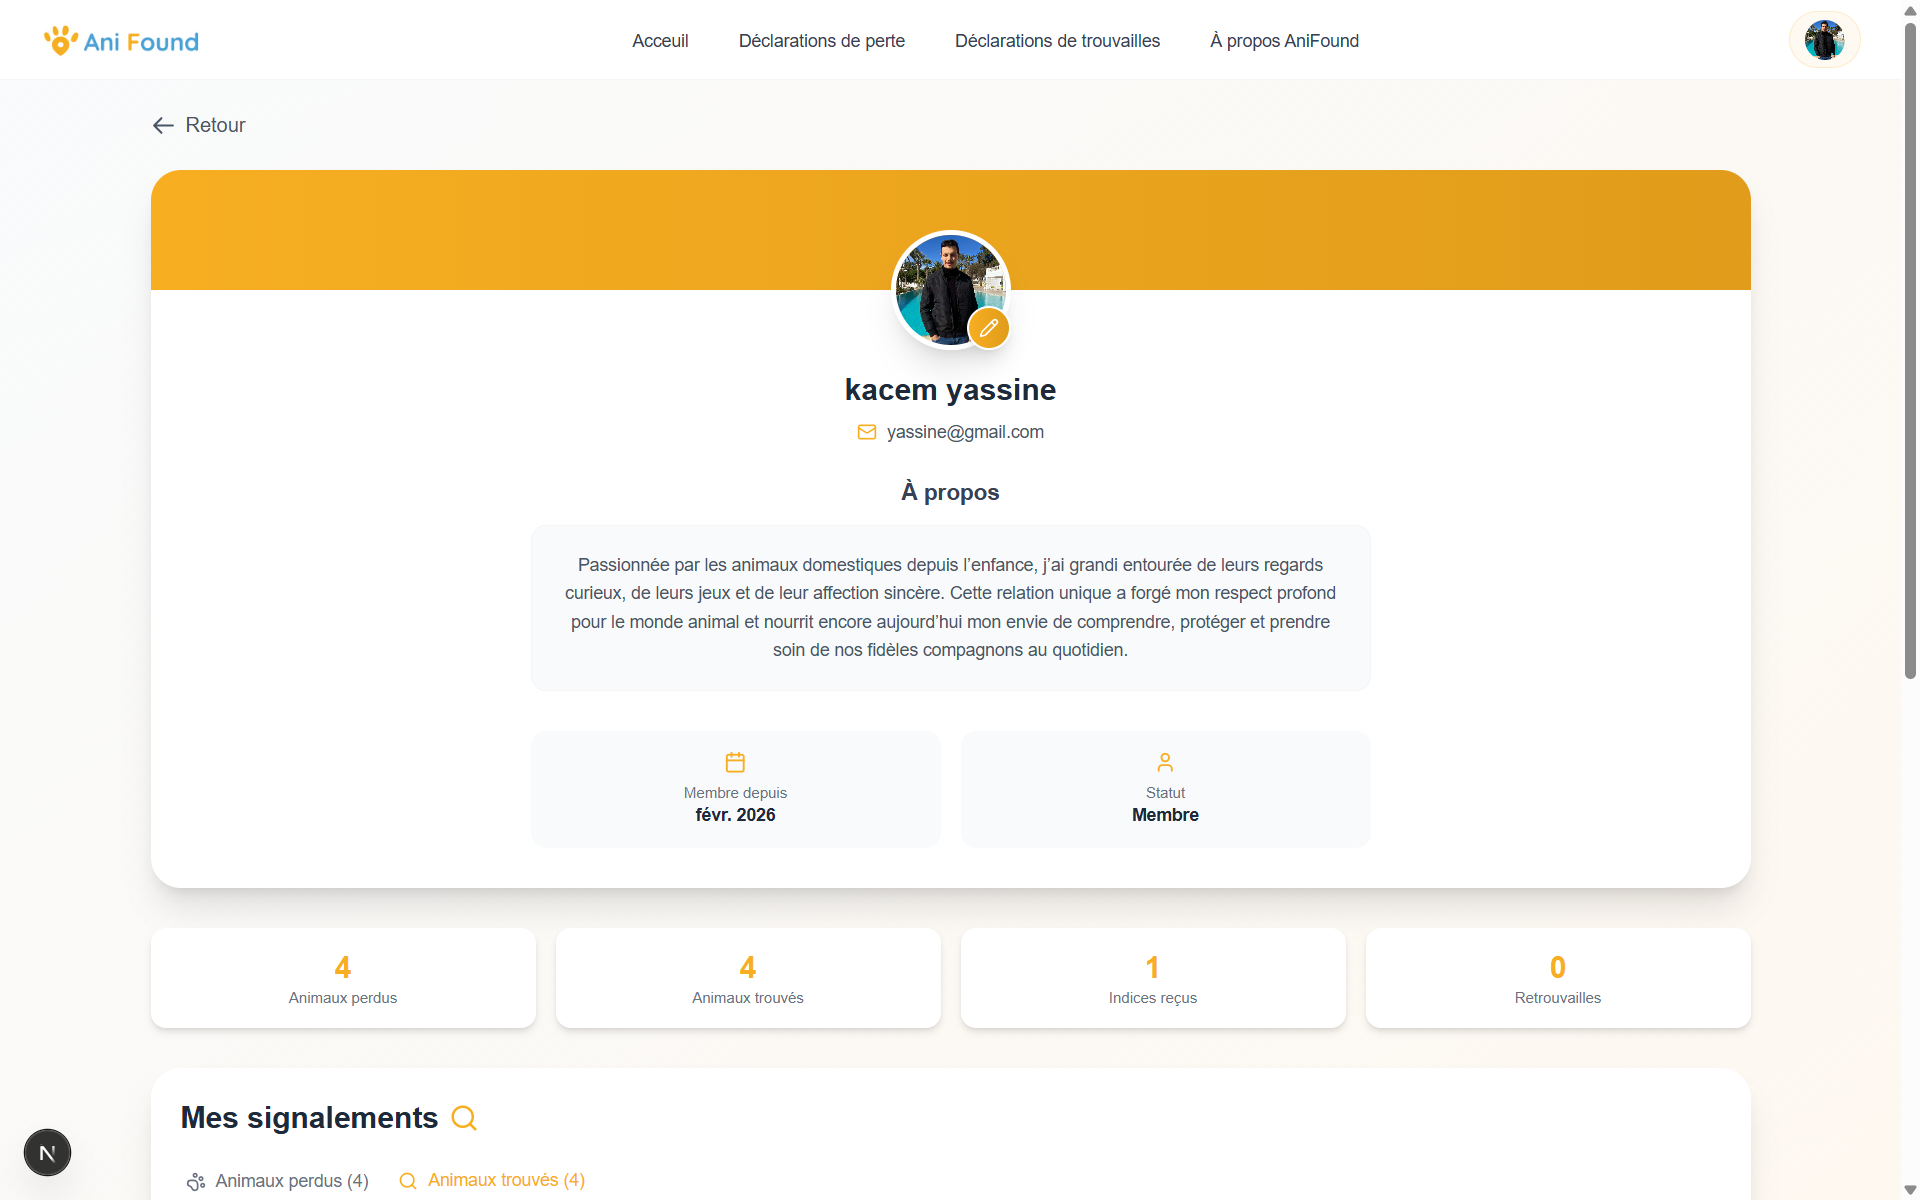
\includegraphics[width=0.77\textwidth]{images/espace anifound profil.png}
    \caption{Interface de l’espace AniFound et gestion du profil}
    \label{fig:espace_anifound_profil}
\end{figure}

\newpage 

\subsubsection{Interface de gestion de mes déclarations de perte et de trouvaille}

La figure \ref{fig:mes_signalements} illustre la gestion des déclarations personnelles de perte et de trouvaille.

\begin{figure}[h!]
    \centering
    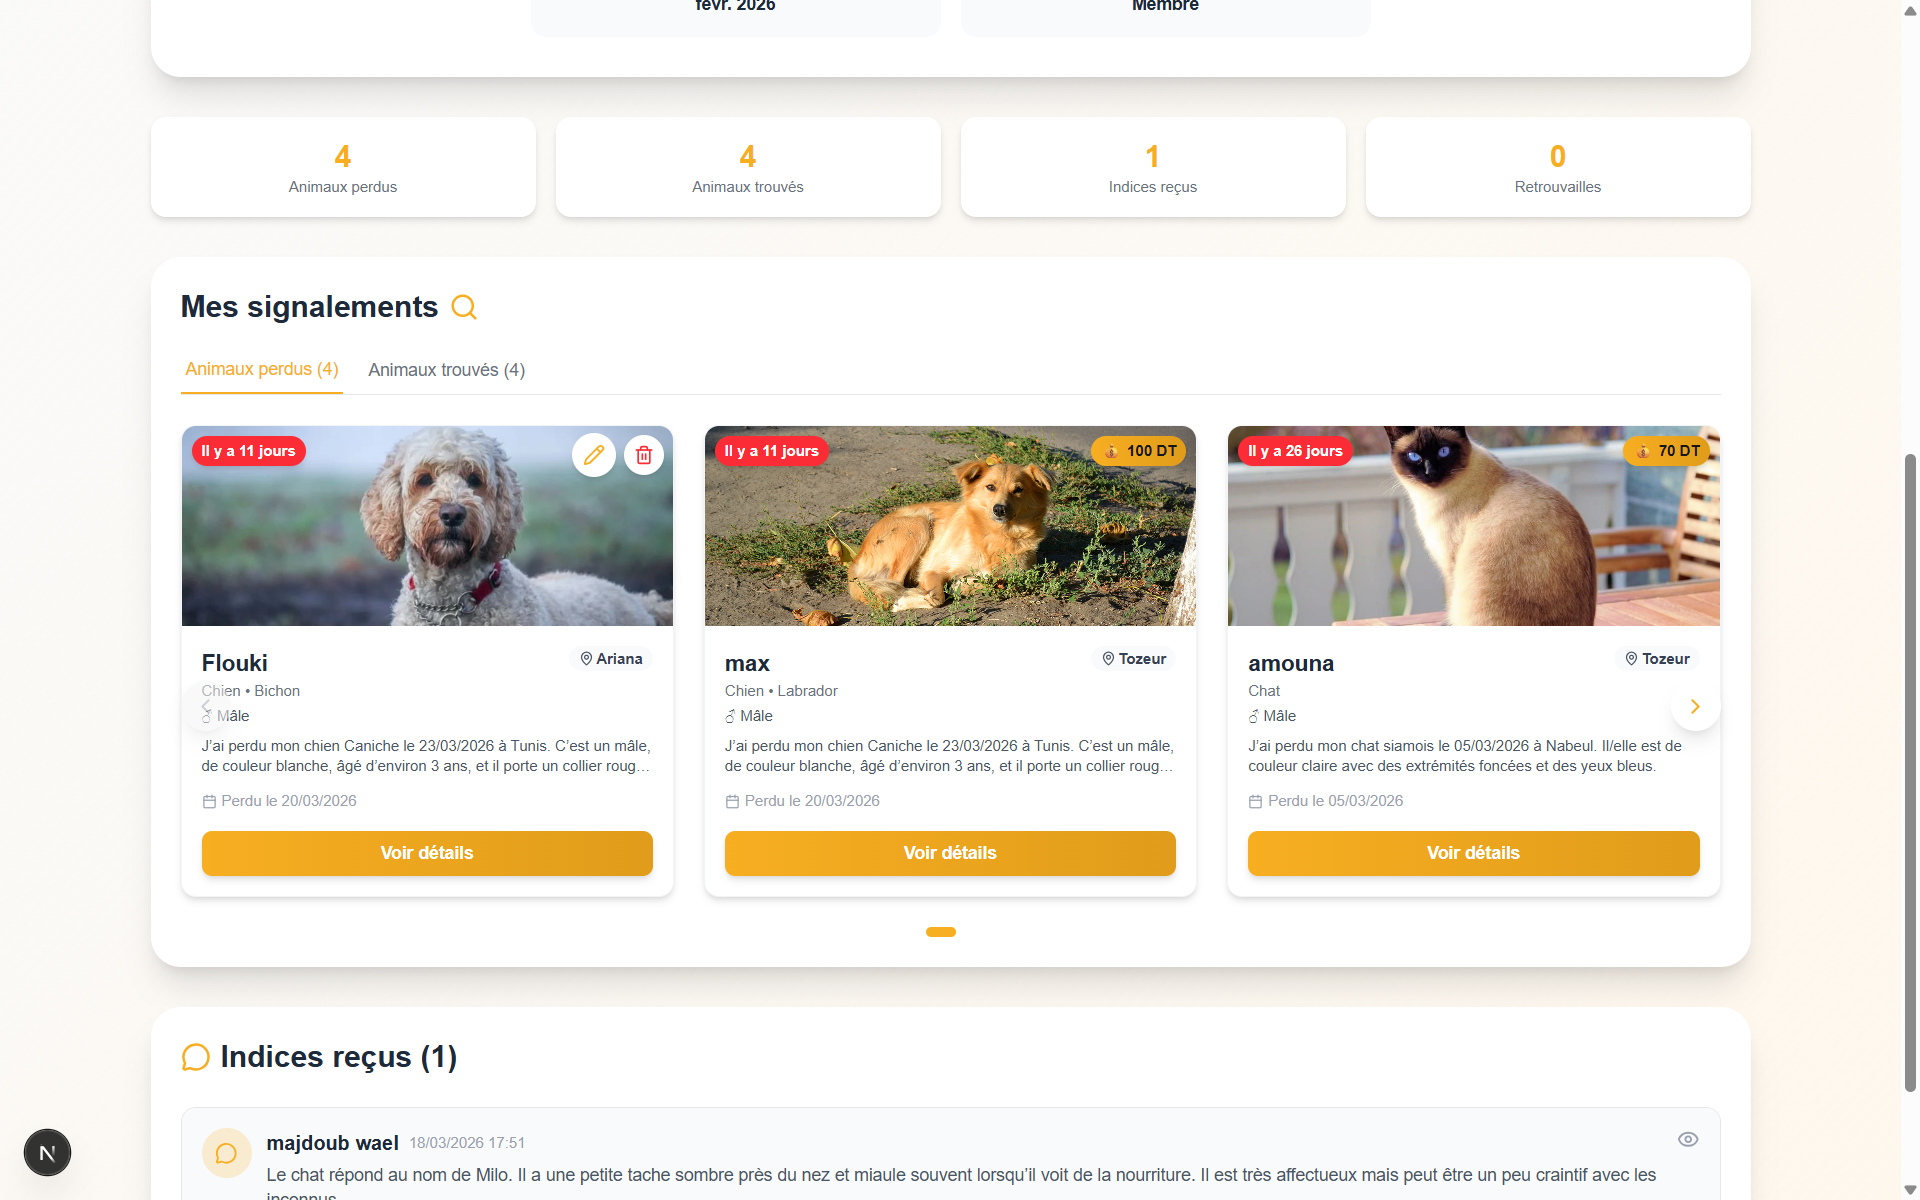
\includegraphics[width=0.87\textwidth]{images/mes signalements.png}
    \caption{Interface de gestion de mes déclarations de perte et de trouvaille}
    \label{fig:mes_signalements}
\end{figure} 

\subsubsection{Interfaces de modification et suppression d’une déclaration de perte ou de trouvaille}

La figure \ref{fig:modif_suppression_declaration} illustre les interfaces de modification et de suppression d’une déclaration.

\begin{figure}[h!]
    \centering
    
    \begin{minipage}{0.51\textwidth}
        \centering
        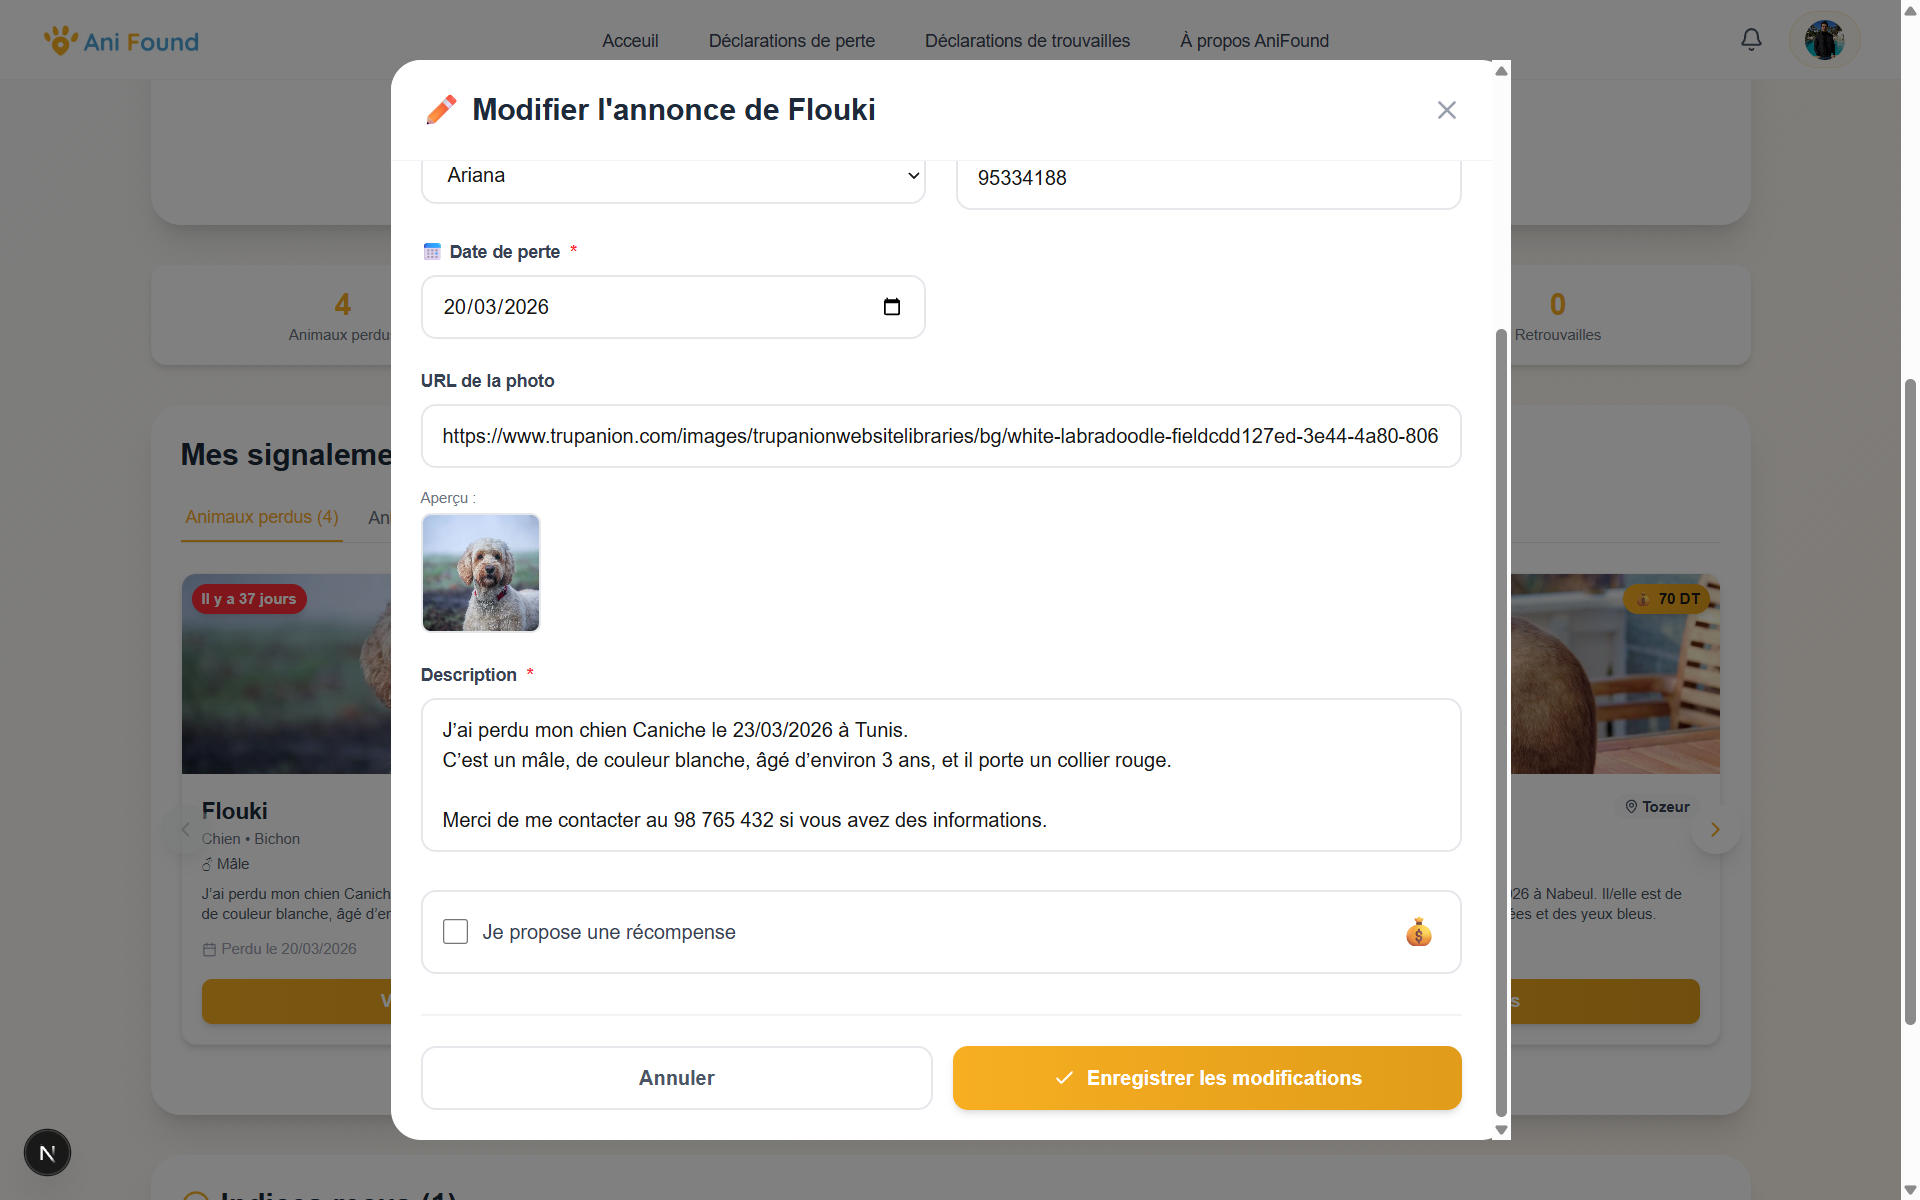
\includegraphics[width=0.77\textwidth]{images/modifer declaration.png}
        \caption{Interface de modification d’une déclaration de perte ou de trouvaille}
        \label{fig:modif_declaration}
    \end{minipage}
    \hfill
    \begin{minipage}{0.48\textwidth}
        \centering
        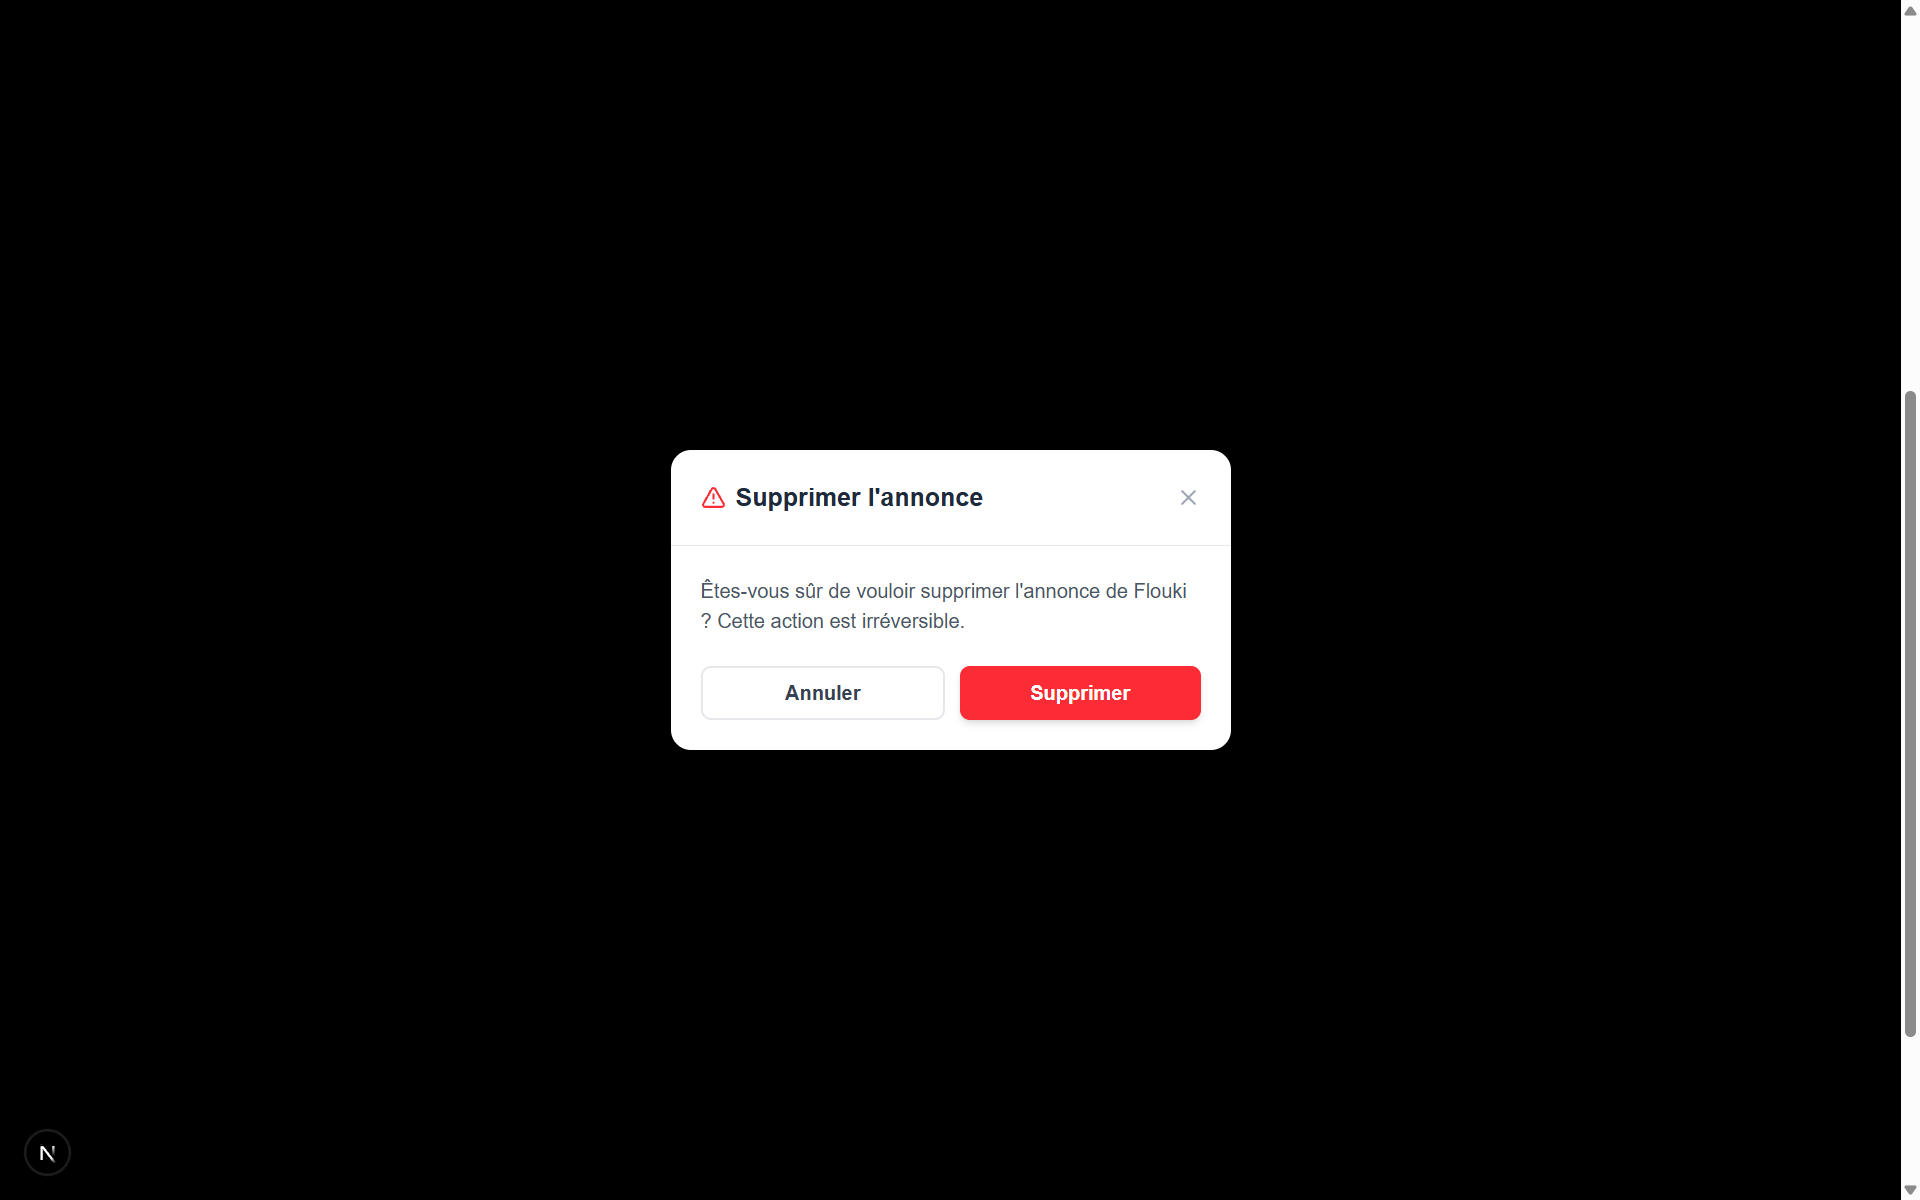
\includegraphics[width=0.77\textwidth]{images/suppression decalaration.png}
        \caption{Interface de suppression d’une déclaration de perte ou de trouvaille}
        \label{fig:suppression_declaration}
    \end{minipage}

\end{figure} 

\newpage 

\subsubsection{Interface des notifications reçues}

La figure \ref{fig:notifications_anifound} illustre une notification reçue concernant un indice lié à une déclaration de trouvaille.

\begin{figure}[h!]
    \centering
    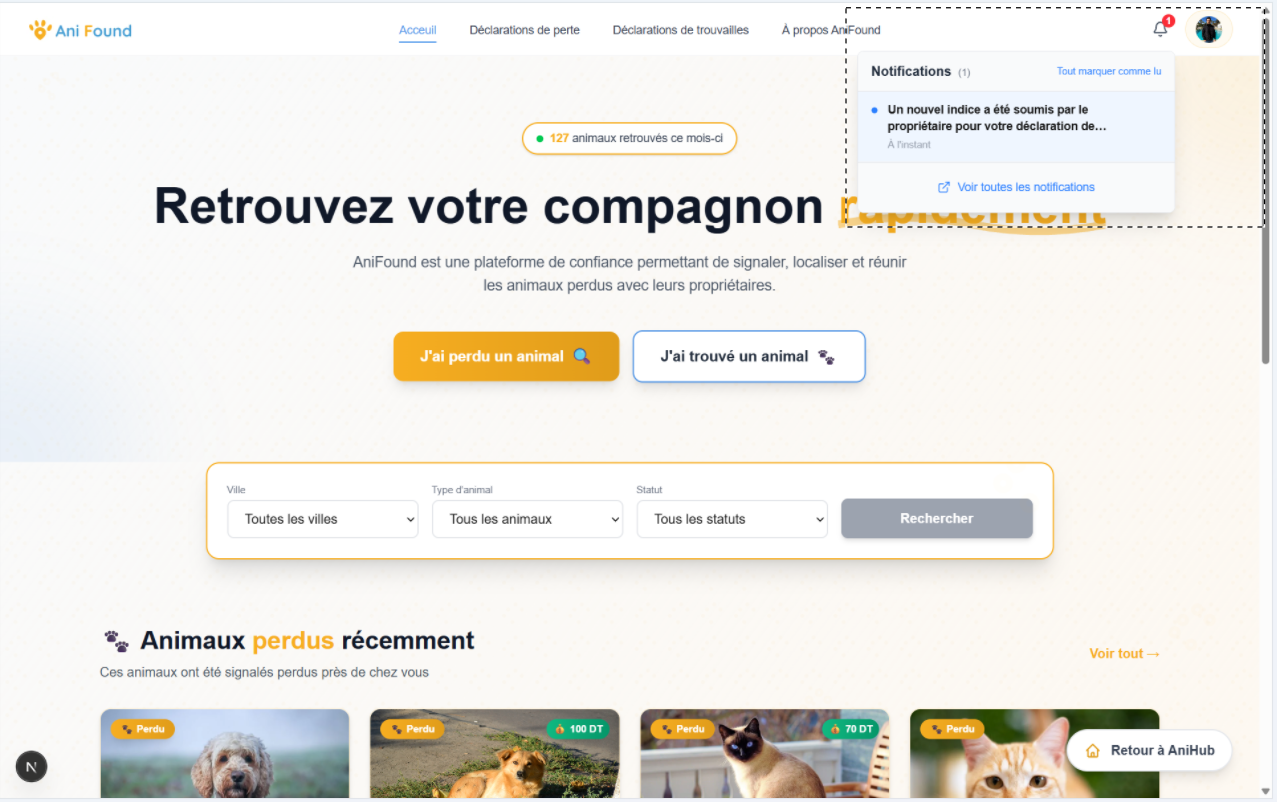
\includegraphics[width=0.77\textwidth]{images/notif anifound.png}
    \caption{Interface des notifications reçues}
    \label{fig:notifications_anifound}
\end{figure}

\subsubsection{Interface des indices reçus pour une déclaration de trouvaille}

La figure \ref{fig:indices_recus} illustre un indice reçu pour une déclaration de trouvaille.

\begin{figure}[h!]
    \centering
    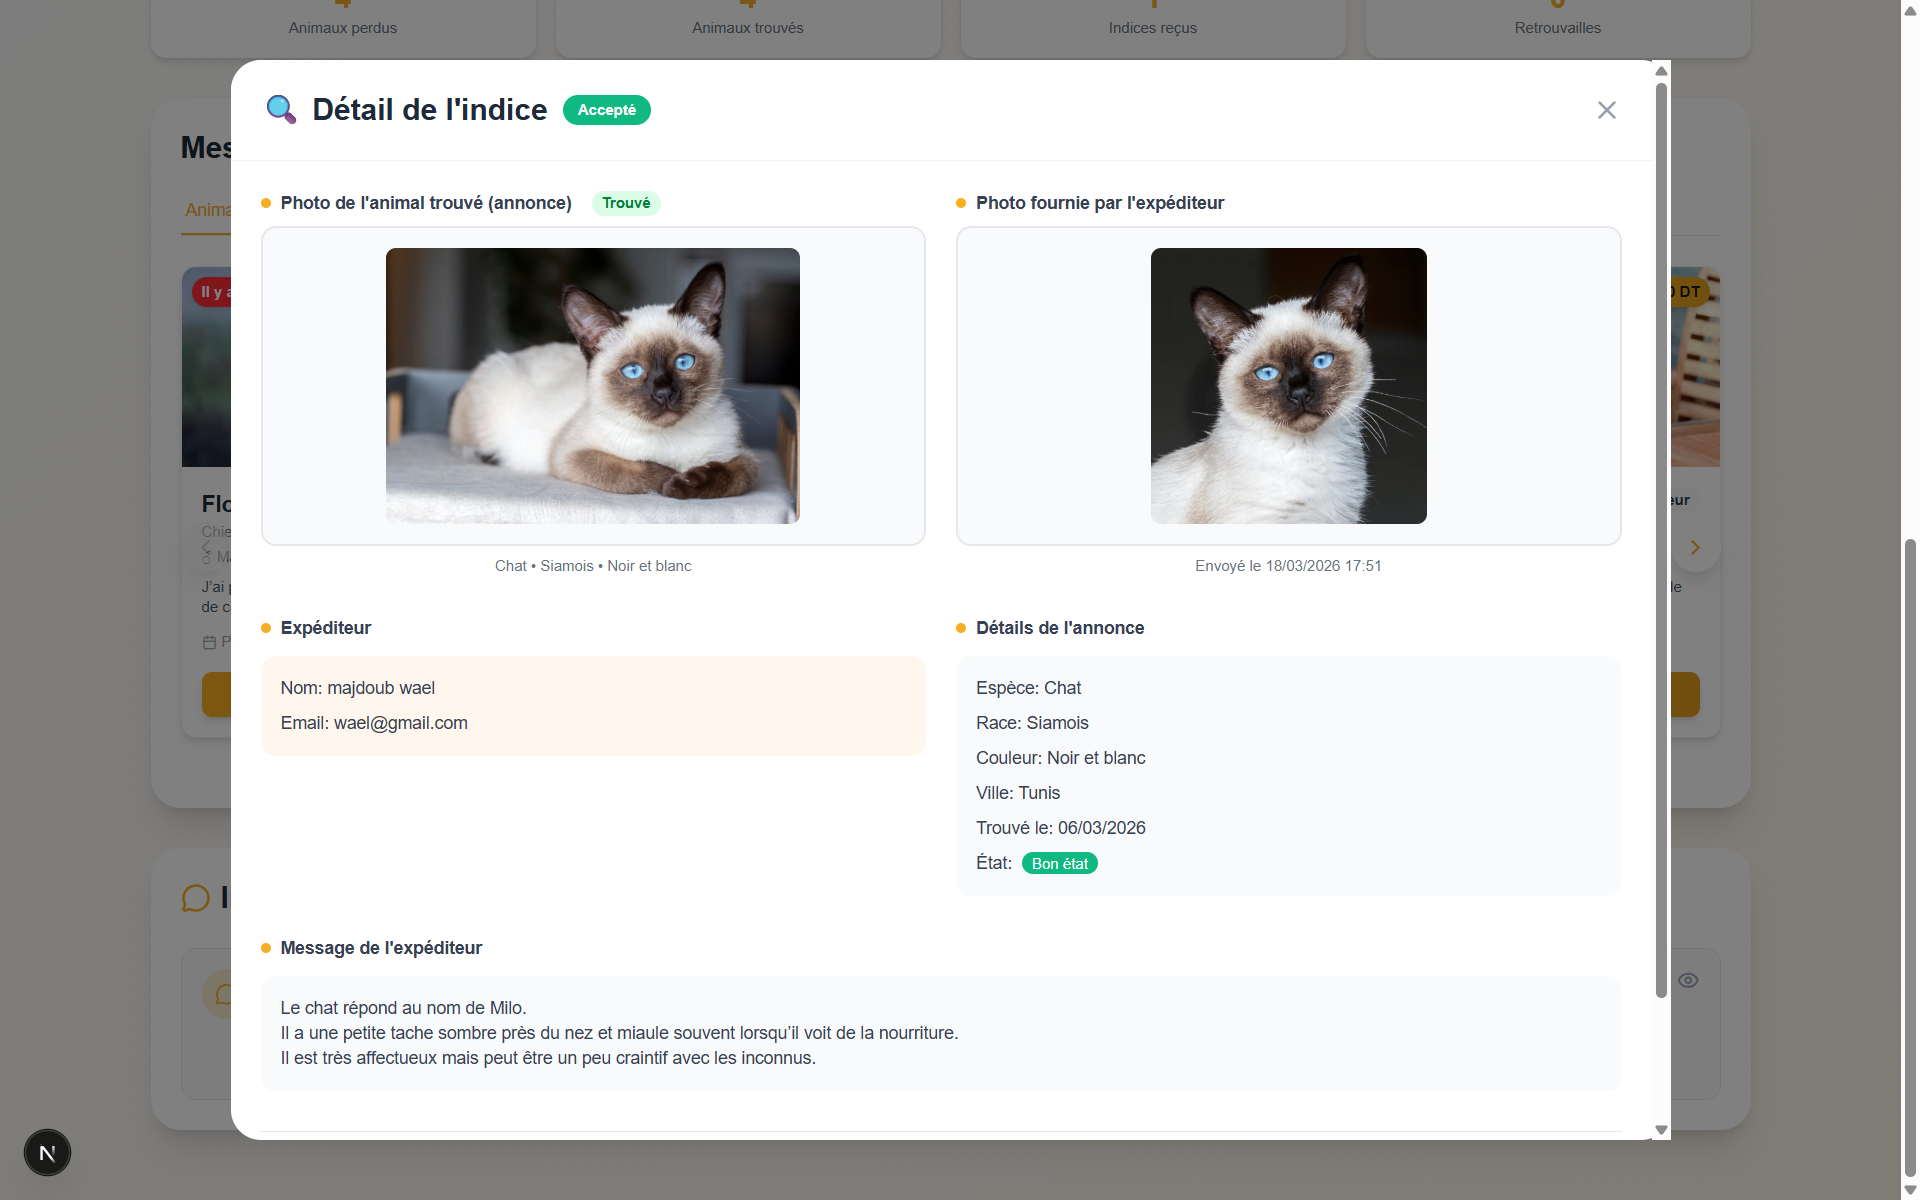
\includegraphics[width=0.77\textwidth]{images/indice recu.png}
    \caption{Interface des indices reçus pour une déclaration de trouvaille}
    \label{fig:indices_recus}
\end{figure}

\newpage
\section{Conclusion}

Ce chapitre a permis de présenter la première release du projet AniHub. Cette release contient trois sprints : le sprint 1 consacré à l’authentification et à l’administration, ainsi que les sprints 2 et 3 dédiés aux modules AniMatch et AniFound. Nous avons détaillé les différentes fonctionnalités développées à travers ces sprints, en mettant en évidence les besoins fonctionnels, la conception ainsi que la réalisation des principales interfaces utilisateur. Cette phase a contribué à mettre en place les principaux mécanismes d’authentification, de mise en relation et de gestion des animaux perdus ou trouvés au sein du système.